\documentclass[a4paper,12pt,twoside]{memoir}

% Castellano
\usepackage[spanish,es-tabla]{babel}
\selectlanguage{spanish}
\usepackage[utf8]{inputenc}
\usepackage[T1]{fontenc}
\usepackage{lmodern} % scalable font
\usepackage{microtype}
\usepackage{placeins}

\RequirePackage{booktabs}
\RequirePackage[table]{xcolor}
\RequirePackage{xtab}
\RequirePackage{multirow}

% Links
\PassOptionsToPackage{hyphens}{url}\usepackage[colorlinks]{hyperref}
\hypersetup{
	allcolors = {red}
}

% Ecuaciones
\usepackage{amsmath}

% Rutas de fichero / paquete
\newcommand{\ruta}[1]{{\sffamily #1}}

% Párrafos
\nonzeroparskip

% Huérfanas y viudas
\widowpenalty100000
\clubpenalty100000

% Evitar solapes en el header
\nouppercaseheads

% Imagenes
\usepackage{graphicx}
\newcommand{\imagen}[2]{
	\begin{figure}[!h]
		\centering
		\includegraphics[width=0.9\textwidth]{#1}
		\caption{#2}\label{fig:#1}
	\end{figure}
	\FloatBarrier
}

\newcommand{\imagenflotante}[2]{
	\begin{figure}%[!h]
		\centering
		\includegraphics[width=0.9\textwidth]{#1}
		\caption{#2}\label{fig:#1}
	\end{figure}
}



% El comando \figura nos permite insertar figuras comodamente, y utilizando
% siempre el mismo formato. Los parametros son:
% 1 -> Porcentaje del ancho de página que ocupará la figura (de 0 a 1)
% 2 --> Fichero de la imagen
% 3 --> Texto a pie de imagen
% 4 --> Etiqueta (label) para referencias
% 5 --> Opciones que queramos pasarle al \includegraphics
% 6 --> Opciones de posicionamiento a pasarle a \begin{figure}
\newcommand{\figuraConPosicion}[6]{%
  \setlength{\anchoFloat}{#1\textwidth}%
  \addtolength{\anchoFloat}{-4\fboxsep}%
  \setlength{\anchoFigura}{\anchoFloat}%
  \begin{figure}[#6]
    \begin{center}%
      \Ovalbox{%
        \begin{minipage}{\anchoFloat}%
          \begin{center}%
            \includegraphics[width=\anchoFigura,#5]{#2}%
            \caption{#3}%
            \label{#4}%
          \end{center}%
        \end{minipage}
      }%
    \end{center}%
  \end{figure}%
}

%
% Comando para incluir imágenes en formato apaisado (sin marco).
\newcommand{\figuraApaisadaSinMarco}[5]{%
  \begin{figure}%
    \begin{center}%
    \includegraphics[angle=90,height=#1\textheight,#5]{#2}%
    \caption{#3}%
    \label{#4}%
    \end{center}%
  \end{figure}%
}
% Para las tablas
\newcommand{\otoprule}{\midrule [\heavyrulewidth]}
%
% Nuevo comando para tablas pequeñas (menos de una página).
\newcommand{\tablaSmall}[5]{%
 \begin{table}
  \begin{center}
   \rowcolors {2}{gray!35}{}
   \begin{tabular}{#2}
    \toprule
    #4
    \otoprule
    #5
    \bottomrule
   \end{tabular}
   \caption{#1}
   \label{tabla:#3}
  \end{center}
 \end{table}
}

%
%Para el float H de tablaSmallSinColores
\usepackage{float}

%
% Nuevo comando para tablas pequeñas (menos de una página).
\newcommand{\tablaSmallSinColores}[5]{%
 \begin{table}[H]
  \begin{center}
   \begin{tabular}{#2}
    \toprule
    #4
    \otoprule
    #5
    \bottomrule
   \end{tabular}
   \caption{#1}
   \label{tabla:#3}
  \end{center}
 \end{table}
}

\newcommand{\tablaApaisadaSmall}[5]{%
\begin{landscape}
  \begin{table}
   \begin{center}
    \rowcolors {2}{gray!35}{}
    \begin{tabular}{#2}
     \toprule
     #4
     \otoprule
     #5
     \bottomrule
    \end{tabular}
    \caption{#1}
    \label{tabla:#3}
   \end{center}
  \end{table}
\end{landscape}
}

%
% Nuevo comando para tablas grandes con cabecera y filas alternas coloreadas en gris.
\newcommand{\tabla}[6]{%
  \begin{center}
    \tablefirsthead{
      \toprule
      #5
      \otoprule
    }
    \tablehead{
      \multicolumn{#3}{l}{\small\sl continúa desde la página anterior}\\
      \toprule
      #5
      \otoprule
    }
    \tabletail{
      \hline
      \multicolumn{#3}{r}{\small\sl continúa en la página siguiente}\\
    }
    \tablelasttail{
      \hline
    }
    \bottomcaption{#1}
    \rowcolors {2}{gray!35}{}
    \begin{xtabular}{#2}
      #6
      \bottomrule
    \end{xtabular}
    \label{tabla:#4}
  \end{center}
}

%
% Nuevo comando para tablas grandes con cabecera.
\newcommand{\tablaSinColores}[6]{%
  \begin{center}
    \tablefirsthead{
      \toprule
      #5
      \otoprule
    }
    \tablehead{
      \multicolumn{#3}{l}{\small\sl continúa desde la página anterior}\\
      \toprule
      #5
      \otoprule
    }
    \tabletail{
      \hline
      \multicolumn{#3}{r}{\small\sl continúa en la página siguiente}\\
    }
    \tablelasttail{
      \hline
    }
    \bottomcaption{#1}
    \begin{xtabular}{#2}
      #6
      \bottomrule
    \end{xtabular}
    \label{tabla:#4}
  \end{center}
}

%
% Nuevo comando para tablas grandes sin cabecera.
\newcommand{\tablaSinCabecera}[5]{%
  \begin{center}
    \tablefirsthead{
      \toprule
    }
    \tablehead{
      \multicolumn{#3}{l}{\small\sl continúa desde la página anterior}\\
      \hline
    }
    \tabletail{
      \hline
      \multicolumn{#3}{r}{\small\sl continúa en la página siguiente}\\
    }
    \tablelasttail{
      \hline
    }
    \bottomcaption{#1}
  \begin{xtabular}{#2}
    #5
   \bottomrule
  \end{xtabular}
  \label{tabla:#4}
  \end{center}
}



\definecolor{cgoLight}{HTML}{EEEEEE}
\definecolor{cgoExtralight}{HTML}{FFFFFF}

%
% Nuevo comando para tablas grandes sin cabecera.
\newcommand{\tablaSinCabeceraConBandas}[5]{%
  \begin{center}
    \tablefirsthead{
      \toprule
    }
    \tablehead{
      \multicolumn{#3}{l}{\small\sl continúa desde la página anterior}\\
      \hline
    }
    \tabletail{
      \hline
      \multicolumn{#3}{r}{\small\sl continúa en la página siguiente}\\
    }
    \tablelasttail{
      \hline
    }
    \bottomcaption{#1}
    \rowcolors[]{1}{cgoExtralight}{cgoLight}

  \begin{xtabular}{#2}
    #5
   \bottomrule
  \end{xtabular}
  \label{tabla:#4}
  \end{center}
}




\graphicspath{ {./img/} }

% Capítulos
\chapterstyle{bianchi}
\newcommand{\capitulo}[2]{
	\setcounter{chapter}{#1}
	\setcounter{section}{0}
	\setcounter{figure}{0}
	\setcounter{table}{0}
	\chapter*{#2}
	\addcontentsline{toc}{chapter}{#2}
	\markboth{#2}{#2}
}

% Apéndices
\renewcommand{\appendixname}{Apéndice}
\renewcommand*\cftappendixname{\appendixname}

\newcommand{\apendice}[1]{
	%\renewcommand{\thechapter}{A}
	\chapter{#1}
}

\renewcommand*\cftappendixname{\appendixname\ }

% Formato de portada
\makeatletter
\usepackage{xcolor}
\newcommand{\tutor}[1]{\def\@tutor{#1}}
\newcommand{\course}[1]{\def\@course{#1}}
\definecolor{cpardoBox}{HTML}{E6E6FF}
\def\maketitle{
  \null
  \thispagestyle{empty}
  % Cabecera ----------------
\noindent
\includegraphics[width=\textwidth]{cabecera}\vspace{1cm}%
  \vfill
  % Título proyecto y escudo informática ----------------
  \colorbox{cpardoBox}{%
    \begin{minipage}{.8\textwidth}
      \vspace{.5cm}\Large
      \begin{center}
      \textbf{TFG del Grado en Ingeniería Informática}\vspace{.6cm}\\
      \textbf{\LARGE\@title{}}
      \end{center}
      \vspace{.2cm}
    \end{minipage}

  }%
  \hfill\begin{minipage}{.20\textwidth}
    
\includegraphics[width=\textwidth]{escudoInfor}
  \end{minipage}
  \vfill
  % Datos de alumno, curso y tutores ------------------
  \begin{center}%
  {%
    \noindent\LARGE
    Presentado por \@author{}\\ 
    en Universidad de Burgos --- \@date{}\\
    Tutor: \@tutor{}\\
  }%
  \end{center}%
  \null
  \cleardoublepage
  }
\makeatother


% Datos de portada
\title{título del TFG \\Documentación Técnica}
\author{nombre alumno}
\tutor{nombre tutor}
\date{\today}

\begin{document}

\maketitle



\cleardoublepage



%%%%%%%%%%%%%%%%%%%%%%%%%%%%%%%%%%%%%%%%%%%%%%%%%%%%%%%%%%%%%%%%%%%%%%%%%%%%%%%%%%%%%%%%



\frontmatter


\clearpage

% Indices
\tableofcontents

\clearpage

\listoffigures

\clearpage

\listoftables

\clearpage

\mainmatter

\appendix

\apendice{Plan de Proyecto Software}

\section{Introducción}

Este proyecto ha estado marcado por pequeñas y grandes variaciones en el código y el objetivo, debido a su naturaleza como un estudio profundo del algoritmo TRACLUS. Estas modificaciones y adaptaciones han sido gestionadas gracias a la implementación de metodologías ágiles durante todo el desarrollo. 

En este apartado se relatará cómo se organizó el proyecto a lo largo del tiempo, detallando las estimaciones realizadas, las tareas planificadas y los resultados obtenidos en cada etapa.

\section{Planificación temporal}

El proyecto se estructuró en sprints de entre quince y veinte días cada uno. Esta metodología ágil permitió dividir el trabajo en ciclos cortos y manejables, lo que facilitó la adaptación a los cambios, la retroalimentación constante y la mejora continua en el desarrollo del software.

Cada sprint incluyó la planificación, ejecución y revisión de tareas específicas que se enfocaban en aspectos clave del proyecto, asegurando un progreso constante y alineado con los objetivos generales.

\subsection{Primer \textit{sprint} (14-12-2023 / 17-01-2024)}

El proyecto comenzó oficialmente con la primera reunión, en la que se establecieron las bases iniciales para el desarrollo. En esta etapa se definieron los siguientes puntos clave:

\begin{itemize}
    \item \textbf{Selección del algoritmo:} Se acordó que el foco principal del proyecto sería el algoritmo TRACLUS, con el objetivo de estudiarlo, implementarlo y evaluar posibles variantes.
    \item \textbf{Estudio de la base teórica:} Se identificaron y seleccionaron las fuentes bibliográficas fundamentales, incluyendo el artículo original de TRACLUS y otras investigaciones relacionadas que pudieran servir como referencia teórica.
    \item \textbf{Definición del objetivo final:} Se estableció que el producto final sería una aplicación web que permitiera visualizar y comparar los resultados del algoritmo TRACLUS con diferentes configuraciones e integraciones.
    \item \textbf{Selección de herramientas:} Se eligieron las herramientas clave para el desarrollo:
        \begin{itemize}
            \item \textbf{Lenguaje de programación:} Python, debido a su potencia en el cálculo numérico, amplia biblioteca para el desarrollo de algoritmos y existencia de implementaciones previas del algoritmo TRACLUS (\texttt{TRACLUS\_library}).
            \item \textbf{Framework para la aplicación web:} Dash, una biblioteca de Python diseñada para la representación interactiva de datos gráficos.
            \item \textbf{Sistema de control de versiones:} GitHub, para almacenar el código, registrar cambios y gestionar el flujo de tareas.
        \end{itemize}
    \item \textbf{Plazos y flujo de trabajo:} Se establecieron reuniones periódicas para evaluar el progreso y ajustar la planificación si fuera necesario.
\end{itemize}

Durante este sprint, se planificaron las siguientes tareas:

\begin{enumerate}
    \item Estudiar la base teórica para comprender en detalle el funcionamiento del algoritmo TRACLUS y sus fundamentos matemáticos.
    \item Preparar una estructura base para documentar adecuadamente el proyecto a medida que avanzara.
    \item Realizar una primera carga de datos de prueba para evaluar el formato necesario y posibles librerías adicionales.
    \item Seleccionar las librerías para la representación gráfica de los datos y realizar una prueba inicial de implementación.
    \item Ejecutar y evaluar la funcionalidad básica de la librería \texttt{TRACLUS\_library}.
\end{enumerate}
\subsubsection{Resultados del primer \textit{sprint}}

Los resultados del primer sprint fueron satisfactorios en términos generales, aunque surgieron algunos desafíos que permitieron identificar áreas de mejora para los siguientes sprints:

\begin{itemize}
    \item \textbf{Estudio inicial de la base teórica:} Se completó el estudio de la literatura relacionada con el algoritmo TRACLUS y sus aplicaciones, lo que proporcionó una comprensión sólida de sus fundamentos y permitió sentar las bases para su implementación.
    
    \item \textbf{Definición de objetivos y herramientas:} Se definieron los objetivos específicos del proyecto y se documentaron las herramientas y tecnologías que se utilizarían a lo largo del desarrollo. Esto incluyó la selección de Python como el lenguaje principal de programación y Dash para la visualización interactiva de datos.
    
    \item \textbf{Primera prueba de carga de datos:} Se realizó una primera prueba de carga de datos, lo que permitió identificar posibles problemas relacionados con el formato y la calidad de los datos. Esto también abrió la discusión sobre la necesidad de limpiar y preparar adecuadamente los datos antes de su procesamiento.
    
    \item \textbf{Investigación de librerías para la representación de mapas:} Se exploraron diversas librerías capaces de representar trayectorias y mapas de calor. Además, se identificaron los primeros problemas de rendimiento, especialmente con la carga inicial de las trayectorias en un mapa. Esto llevó a la necesidad de optimizar esta parte del flujo de trabajo.
    
    \item \textbf{Problemas con la ejecución de \texttt{TRACLUS\_library}:} Aunque se intentó ejecutar la librería \texttt{TRACLUS\_library}, la ejecución no fue exitosa. Esto se debió a la falta de familiaridad con el código base de la librería y la complejidad inherente a su funcionamiento.
\end{itemize}

A pesar de los logros y avances iniciales, se comenzaron a evidenciar las primeras dificultades, principalmente debido al uso de herramientas y tecnologías nuevas, en las cuales no se tenía experiencia previa, y al manejo del gran volumen de datos que se deseaba procesar. 

La estimación inicial para este sprint era de aproximadamente 30 horas, pero al final se emplearon unas 40 horas para completar todas las tareas asignadas. Este desfase en el tiempo se debió principalmente a la curva de aprendizaje de las herramientas y a la necesidad de hacer ajustes en los datos y en las librerías utilizadas.

\subsection{Segundo \textit{sprint} 18-01-2024 / 30-01-2024}

La segunda reunión comenzó con la exposición y discusión sobre los avances y problemas enfrentados en las tareas asignadas durante el primer sprint. A partir de ahora, todas las reuniones seguirían este formato, centradas en la revisión del trabajo realizado y la planificación de las nuevas tareas.

Para este sprint, se tomó en cuenta la tarea no lograda del sprint anterior: la ejecución del algoritmo TRACLUS. En esta fase, se debía estudiar más profundamente cada una de las funciones de la librería \texttt{TRACLUS\_library} y su relación teórica con el algoritmo TRACLUS, con el objetivo de lograr una comprensión más detallada de su funcionamiento y poder implementarlo correctamente.

Además, con el avance en la representación inicial de las trayectorias en los mapas, se buscó añadir nuevas funcionalidades, como la capacidad de hacer zoom o mostrar las trayectorias de diferentes formas, lo que permitiría una mejor visualización de los datos.

Por otro lado, la página web debía comenzar a ser considerada. Se propuso investigar las herramientas más adecuadas para su desarrollo, y se decidieron investigar dos opciones: Plotly Dash y Flask. La tarea consistió en analizar ambas tecnologías y decidir cuál de ellas se adaptaba mejor a las necesidades del proyecto.

Finalmente, se continuó trabajando en la memoria del proyecto, lo cual era una tarea constante a lo largo de todo el trabajo. El registro de investigaciones, avances y decisiones es fundamental para mantener una documentación clara y precisa.

\subsubsection{Resultados del segundo \textit{sprint}}

Los resultados de este segundo sprint fueron los siguientes:

\begin{itemize}
    \item Se profundizó en el estudio de la librería \texttt{TRACLUS\_library}, lo que permitió mejorar el conocimiento de su funcionamiento y relación con el algoritmo TRACLUS.
    
    \item Se implementó un código para probar la ejecución de los datos leídos en el sprint anterior, lo que permitió avanzar en la integración de la librería con los datos.
    
    \item Se decidió utilizar \texttt{Dash} como la librería base para la página web, debido a su capacidad para representar datos de forma interactiva, lo que se ajusta a los objetivos del proyecto.
    
    \item Se comenzó a desarrollar la página web, incluyendo la creación de un prototipo inicial para la visualización de trayectorias.
    
    \item Se priorizó la eficiencia en la carga y ejecución de los mapas de trayectorias, sacrificando algo de calidad visual en favor de tiempos de ejecución más rápidos.
    
    \item Se dedicó tiempo a continuar con la memoria del proyecto, registrando los avances y decisiones tomadas durante este sprint.
\end{itemize}

Se estimaron unas 15 horas para completar este sprint, pero finalmente se emplearon unas 20 horas.

\subsection{Tercer \textit{sprint} 31-01-2024 / 13-02-2024}

En esta reunión se llegó a la conclusión de que, para usar correctamente la librería \texttt{TRACLUS}, se debían realizar pruebas internas más detalladas para entender cómo funciona el algoritmo y qué resultados proporciona. Entre las métricas que se analizaron se incluyeron: cuántas trayectorias se asignaban a cada clúster, cuáles eran los clústeres con más trayectorias, la longitud de los clústeres, cómo se segmentan las trayectorias, y otros datos que podrían ser útiles para la evaluación de los resultados y la representación de las trayectorias.

Además de estudiar la librería, se consideró el hecho de que el algoritmo TRACLUS, aunque no haya sido ampliamente utilizado, existe desde 2007. Por lo tanto, se decidió buscar estudios previos y pseudocódigos de diversas variantes del algoritmo que han sido creadas a lo largo de los años, con el fin de evaluar si podrían implementarse en el futuro para mejorar el proyecto.

Los datos también fueron un punto clave durante este sprint. Hasta ese momento, solo se había estado trabajando con un conjunto de datos de Trayectoria de Taxis, el cual, aunque útil para las pruebas iniciales, era limitado. Por ello, se comenzó a investigar otros conjuntos de datos, como el conjunto de datos Geolife, para explorar su utilidad en los experimentos. Además, se empezaron a crear filtros específicos para asegurar que los experimentos realizados fueran correctos y los resultados adecuados.

Por último, se planteó realizar un cambio en uno de los mapas que se habían probado inicialmente, el mapa de calor. Este mapa se rediseñó para mejorar su visualización y usabilidad.

\subsubsection{Resultados del tercer \textit{sprint}}

Los resultados del tercer sprint fueron los siguientes:

\begin{itemize}
    \item Se identificó que la librería \texttt{TRACLUS} utiliza \texttt{sklearn} para la clusterización, con el algoritmo OPTICS como predeterminado. Esto abrió una vía para continuar la investigación, ya que existen varios algoritmos de clustering que tiene propiedades similares a las de OPTICS.
    
    \item Se analizó y se obtuvo una comprensión adecuada de los datos generados por \texttt{TRACLUS}, lo cual fue útil para la presentación de resultados en la exposición.
    
    \item Se identificaron y evaluaron diversas variantes del algoritmo \texttt{TRACLUS}, como \texttt{N-TRACLUS} y \texttt{ST-TRACLUS}, pero se concluyó que no sería posible implementarlas debido a la limitación de tiempo del proyecto.
    
    \item Se investigó el conjunto de datos Geolife y se observó que su formato era muy diferente al de los datos de trayectorias de taxis, por lo que se decidió dejarlo apartado por el momento. No obstante, se planteó la posibilidad de incluirlo en el futuro, si se consideraba necesario y el tiempo lo permitía.
    
    \item Se rediseñó el mapa de calor para mejorar su visualización. En lugar del diseño original, se optó por un histograma creado con la librería \texttt{numpy}, representado en un mapa, lo que mejoró la claridad de los datos.
    
    \item Se completaron correctamente los filtros necesarios para los experimentos, asegurando que los datos estuvieran bien preparados para su análisis.
\end{itemize}

La estimación inicial de tiempo para este sprint fue de unas 20 horas, pero finalmente se superaron las expectativas, ya que se emplearon más de 30 horas debido al extenso estudio y análisis requerido para comprender la librería, los algoritmos asociados y los datos utilizados.

\subsection{Cuarto \textit{sprint} 14-02-2024 / 27-02-2024}

En esta reunión se discutió cómo deberían ser expuestos correctamente los datos generados por el algoritmo, además de cómo debían ser tratados para evitar problemas como errores de formato. Se decidió que se debían generar estadísticas de manera representativa, utilizando tablas que mostraran todos los datos de un clúster, histogramas y otras visualizaciones. Asimismo, se investigaron algoritmos y librerías que pudieran ayudar a extraer estadísticas complementarias para enriquecer los resultados.

Hasta este punto, los mapas seguían basándose en un conjunto de librerías específico, pero únicamente se había desarrollado el código para representar las trayectorias iniciales en el mapa. Ahora, con el algoritmo TRACLUS ejecutado y conociendo los datos obtenidos, se decidió desarrollar diversos mapas que representaran los cambios y resultados de cada uno de los pasos del algoritmo.

Adicionalmente, se continuó con la investigación teórica sobre el algoritmo TRACLUS y se realizó un registro detallado del conocimiento adquirido. Esto incluyó comentarios y anotaciones en la librería \texttt{TRACLUS}, facilitando revisiones y posibles modificaciones futuras.

\subsubsection{Resultados del cuarto \textit{sprint}}

Los resultados obtenidos en este sprint fueron los siguientes:

\begin{itemize}
    \item Se desarrollaron diversas funciones para mostrar los datos generados por el algoritmo \texttt{TRACLUS}, incluyendo mapas, tablas y diagramas. Algunos de estos resultados fueron descartados, pero otros se consideraron útiles para la exposición final.
    
    \item Se crearon múltiples mapas para representar las trayectorias y los cambios en las distintas etapas del algoritmo. Esto permitió visualizar los pasos del algoritmo de una forma más clara y comprensible.
    
    \item Aunque se investigaron librerías y algoritmos para calcular estadísticas adicionales, no se encontraron resultados que aportaran mejoras significativas al entendimiento de los datos generados.
    
    \item Se realizó un \textit{fork} de la librería \texttt{TRACLUS} y se añadieron comentarios extensos para mejorar la comprensión del código, facilitando su revisión y posibles modificaciones futuras.
    
    \item Se continuó con el análisis teórico de la matemática aplicada en el algoritmo \texttt{TRACLUS}, lo que ayudó a consolidar el conocimiento sobre su funcionamiento.
\end{itemize}

En cuanto a las estimaciones de tiempo, estas dejaron de ser completamente útiles. Esto se debió a las constantes pruebas necesarias del algoritmo \texttt{TRACLUS} para generar mapas, extraer datos y entender su funcionamiento. Estas pruebas resultaron extremadamente lentas, lo que afectó el tiempo total del sprint. Aunque se habían estimado aproximadamente 25 horas para las tareas de este sprint, el tiempo real de trabajo neto superó las 35 horas y en términos de horas brutas contando las esperas, el tiempo total invertido fue significativamente mayor.

\subsection{Quinto \textit{sprint} 28-02-2024 / 13-03-2024}

Hasta este punto, la página web había quedado en segundo plano debido a la prioridad de garantizar el correcto funcionamiento del algoritmo \texttt{TRACLUS}, además de definir qué datos y cómo debían ser expuestos. Con estos aspectos ya avanzados, se decidió comenzar la creación de la página web en su etapa inicial. Esto incluyó la implementación del diseño basado en los prototipos discutidos en reuniones anteriores, evaluando qué era posible y útil, y estableciendo un patrón de diseño estándar a partir de las primeras páginas creadas.

La excesiva demora en las ejecuciones del algoritmo fue otro tema central en esta reunión. Dado que se buscaba analizar grandes volúmenes de datos, era necesario reducir los tiempos de ejecución. En este momento, no se contaba con un conocimiento profundo de las herramientas disponibles en Python para optimizar procesos, por lo que se decidió investigar este aspecto.

Complementariamente, se propuso realizar un análisis de rendimiento de la aplicación, dividiendo las mediciones por funciones, para identificar áreas específicas a mejorar.

Por último, aunque previamente se había descartado implementar variantes del algoritmo \texttt{TRACLUS}, se sugirió investigar algoritmos de clustering que pudieran integrarse al flujo del algoritmo para comparar su rendimiento y resultados.

\subsubsection{Resultados del quinto \textit{sprint}}

Los resultados obtenidos en este sprint fueron los siguientes:

\begin{itemize}
    \item Se avanzó significativamente en el desarrollo de la página web:
        \begin{itemize}
            \item Se creó una página inicial para subir el archivo de datos y seleccionar la cantidad de datos a utilizar.
            \item Tras cargar el archivo, se implementó una página para visualizar los mapas de las trayectorias iniciales.
            \item A través de una barra de navegación, el usuario podía acceder a:
                \begin{itemize}
                    \item Una página para ejecutar el algoritmo \texttt{TRACLUS} (aún no implementado en esta etapa).
                    \item Una página para visualizar los resultados del algoritmo, con mapas actualizados y una tabla de resultados.
                \end{itemize}
        \end{itemize}

    \item Se investigaron herramientas de Python para optimizar procesos, encontrando las siguientes:
        \begin{itemize}
            \item \texttt{numpy} y \texttt{pandas} para realizar operaciones más rápidas mediante paralelización.
            \item \texttt{Threading} para implementar hilos y dividir la ejecución en subprocesos.
        \end{itemize}

    \item El análisis de rendimiento reveló:
        \begin{itemize}
            \item La librería \texttt{TRACLUS} tenía una complejidad \(O(n^2)\) en el cálculo de distancias entre trayectorias, ya que cada una debía compararse con todas las demás.
            \item Otras funciones, como la clusterización, también presentaban tiempos elevados, aunque menos pronunciados, y utilizaban la librería \texttt{scikit-learn}, lo que limitaba las posibilidades de optimización interna.
        \end{itemize}

    \item Se identificaron cinco algoritmos de clustering adecuados para integrar y comparar con el flujo del algoritmo \texttt{TRACLUS}:
        \begin{itemize}
            \item OPTICS
            \item DBSCAN
            \item HDBSCAN
            \item \texttt{SpectralClustering}
            \item \texttt{AgglomerativeClustering}
        \end{itemize}
\end{itemize}

En cuanto a tiempos, se habían estimado 30 horas para este sprint, sin contar las horas de pruebas se cumplieron las estimaciones.

\subsection{Sexto \textit{sprint} 14-03-2024 / 11-04-2024}

Ya teniendo claro como iba a ser el desarrollo de la web se decidio que se debia comtinuar implementando las diferentes funciones planteadas y probar nuevas como cargar mapas con variaciones de aumentos en el mapa.

El rendimiento era en este momento el principal obstaculo y ya se conocion diversas formas de como mejorar esto con el estudio que se hizo en el anterior esprin asi que se planteo intentar reducir el tiempo de caraga todo lo que sepudiera enfocandose en la funcion que media las tres distancias (angular, paralela y perpendicular).

Ademas de todo esto se planteo compara los resultados que daban las funciones de clusting entre ellas.

\subsection{Sexto \textit{sprint} 14-03-2024 / 11-04-2024}

Con un diseño claro para la página web, se decidió continuar implementando las diversas funciones planteadas, además de probar nuevas características, como cargar mapas con diferentes niveles de zoom.

El rendimiento seguía siendo el principal obstáculo, pero gracias al estudio realizado en el sprint anterior, se identificaron formas de mejorar los tiempos de carga. El enfoque principal fue optimizar la función que calculaba las tres distancias fundamentales del algoritmo \texttt{TRACLUS} (angular, paralela y perpendicular).

Finalmente, se planteó comparar los resultados de los distintos algoritmos de \textit{clustering} identificados en el sprint anterior, con el fin de entender sus diferencias y evaluar su impacto en el análisis.

\subsubsection{Resultados del sexto \textit{sprint}}

Los resultados obtenidos fueron los siguientes:

\begin{itemize}
    \item \textbf{Avances en la web:}
        \begin{itemize}
            \item Se continuó con el desarrollo de las funciones principales.
            \item Se descartaron cambios en los mapas debido a problemas de rendimiento.
            \item Se plantearon ajustes en la forma de ejecutar las funciones:
                \begin{itemize}
                    \item Separar la ejecución del algoritmo \texttt{TRACLUS} de la visualización de los mapas, ya que realizarlas en la misma página provocaba problemas al volver a los datos cargados previamente.
                \end{itemize}
            \item Se trasladaron los estilos integrados en los archivos de Python a un archivo CSS, mejorando la comprensión y mantenibilidad del código.
        \end{itemize}
        
    \item \textbf{Comparación de algoritmos de \textit{clustering}:}
        \begin{itemize}
            \item Se evidenciaron diferencias significativas entre los algoritmos evaluados (OPTICS, DBSCAN, HDBSCAN, \texttt{SpectralClustering} y \texttt{AgglomerativeClustering}).
            \item Cada algoritmo utilizaba diferentes enfoques para segmentar los datos y construir los clústeres, lo que resultaba en variaciones notables en los resultados.
            \item Se identificó que los algoritmos permitían ajustar parámetros para modificar el procesamiento y los resultados obtenidos.
        \end{itemize}
        
    \item \textbf{Optimización del rendimiento:}
        \begin{itemize}
            \item La optimización fue una de las tareas más desafiantes debido a las limitaciones de Python en la creación de hilos y la paralelización en comparación con otros lenguajes como Java.
            \item Se realizaron pruebas con diferentes librerías, pero los cálculos matemáticos mostraban variaciones en los resultados dependiendo de la librería utilizada.
            \item Se ejecutaron cientos de pruebas del algoritmo \texttt{TRACLUS} durante este sprint, ya que cada tarea requería verificaciones constantes, lo que incrementó los tiempos significativamente.
        \end{itemize}
\end{itemize}  
     
Inicialmente se estimaron alrededor de 60 horas para este sprint. Sin embargo, las horas reales superaron ampliamente la estimación, siendo aproximadamente tres veces mayor debido a las pruebas continuas y los desafíos encontrados.

\subsection{Séptimo \textit{sprint} 12-04-2024 / ---}

En este punto, el proyecto experimentó una pausa significativa debido a un grave accidente sufrido, lo cual me impidió continuar con el desarrollo durante el resto del semestre. 

Por lo tanto, este séptimo \textit{sprint} se considera una pausa en el proyecto, sin avances ni resultados relevantes que reportar.

\subsection{Octavo \textit{sprint} 09-09-2024 / 16-10-2024}

El proyecto se retomó con el comienzo del primer semestre del nuevo curso. Debido al tiempo transcurrido y al tiempo limitado al inicio del semestre, la reunión formal se llevó a cabo el 27 de septiembre. Sin embargo, el \textit{sprint} se considera iniciado desde el momento en que se reactivaron las actividades relacionadas con el proyecto.

Para comenzar, se revisaron todos los documentos externos e internos relacionados con el proyecto con el fin de ponerse al día y continuar sin errores derivados de la pérdida de conocimiento durante la pausa.

Durante la reunión, se evaluó el estado de avance del proyecto, las tareas propuestas en la última reunión previa al accidente y cómo proceder a partir de allí. Las decisiones y tareas principales planteadas incluyeron:

\begin{itemize}
    \item Pulir y comprobar las funcionalidades existentes de la página web, dividiendo correctamente sus partes para mayor claridad y eficiencia.
    \item Cambiar la página inicial, permitiendo al usuario elegir entre crear un nuevo experimento o cargar uno ya existente. Se planteó implementar un mecanismo para guardar y reutilizar experimentos previamente creados.
    \item Añadir la funcionalidad de descargar los resultados obtenidos tras la ejecución del algoritmo \textit{TRACLUS}, entregando los datos al usuario en formato \texttt{.zip}.
    \item Implementar correctamente el algoritmo \textit{TRACLUS} en la aplicación. A partir de este momento, el algoritmo se ejecutaría en la pantalla de carga de datos, unificando la interacción con los datos para reducir tiempos de espera.
    \item Finalizar la comparación de algoritmos de \textit{clustering} para determinar cuáles podrían ser integrados en la aplicación.
    \item Continuar el desarrollo y la documentación de la memoria.
\end{itemize}

\subsubsection{Resultados del octavo \textit{sprint}}

Los avances en la aplicación fueron significativos. Se implementaron todas las nuevas funcionalidades propuestas, destacando:

\begin{itemize}
    \item Se integró correctamente el algoritmo \textit{TRACLUS} en la aplicación, permitiendo su ejecución y el tratamiento de datos desde la pantalla de carga de datos. Los resultados obtenidos tras la ejecución del algoritmo se guardan automáticamente dentro del programa.
    \item Se creó una nueva página de inicio que permite cargar datos de experimentos anteriores o dirigirse a la pantalla de carga para comenzar un nuevo experimento.
    \item La funcionalidad de descarga de datos se implementó con éxito. Los datos, ya sean nuevos o previamente cargados, pueden descargarse desde la visualización de resultados a través de la barra de navegación, siendo entregados en un archivo comprimido \texttt{.zip}.
    \item La barra de navegación fue reformada para garantizar que las páginas solo sean accesibles cuando sea posible, según el estado actual de los datos y las acciones realizadas.
    \item Se analizaron los parámetros configurables en \texttt{sklearn} que provocan cambios en los algoritmos de clustering.
        \item Algunos parámetros útiles son específicos y están interrelacionados con otros datos de entrada.
    \item Se continuó trabajando en la memoria del proyecto para documentar los avances.
\end{itemize}

En este \textit{sprint}, las estimaciones de tiempo fueron más precisas gracias a una mayor división en las tareas. Se estimaron 45 horas de trabajo, que prácticamente coincidieron con las horas efectivamente dedicadas, sin contar el tiempo necesario para recuperar conocimientos previos al accidente.

\subsection{Noveno \textit{sprint} 17-10-2024 / 03-11-2024}

Ya teniendo los resultados de los diferentes algoritmos de \textit{clustering} y los datos que causaban modificaciones en los cálculos, se propuso implementar una nueva página para la web. Esta estaría ubicada en la sección de creación de un nuevo experimento, y su función sería darle al usuario la posibilidad de elegir qué algoritmos y con qué parámetros ejecutar el experimento, permitiendo realizar comparaciones.

Además, la aplicación había avanzado rápidamente, dejando el formato relegado a favor de la velocidad, lo cual, aunque útil inicialmente, podría generar problemas en el futuro en cuanto a mantenimiento y comprensión. Por tanto, se propuso remodelarla para adherirse lo mejor posible al modelo Vista-Controlador (MVC).

Finalmente, se identificó que los datos devueltos no eran del todo satisfactorios, por lo que se propuso reformar esta parte y buscar formas más claras y útiles de mostrarlos.

\subsubsection{Resultados del noveno \textit{sprint}}

\begin{itemize}
    \item Se implementó una nueva pantalla entre la página de inicio y la página de carga de datos:
    \begin{itemize}
        \item La pantalla permite seleccionar entre los cinco algoritmos de \textit{clustering}, pudiendo elegir desde uno hasta todos.
        \item Es obligatorio integrar los datos de todos los algoritmos seleccionados.
        \item Una vez completada esta acción, se accede a la página de carga de datos donde se introducen los datos y se ejecuta el algoritmo TRACLUS tantas veces como algoritmos hayan sido seleccionados.
        \item Esta funcionalidad incrementa el tiempo de ejecución, pero permite al usuario comparar los resultados de los distintos algoritmos.
    \end{itemize}
    
    \item Para que la representación de los datos funcione correctamente:
    \begin{itemize}
        \item Se crearon desplegables que permiten al usuario seleccionar qué algoritmo utilizar para cada representación de datos.
        \item Estos desplegables se activan o desactivan dependiendo de si el algoritmo ha sido utilizado.
    \end{itemize}
    
    \item Se reorganizó la estructura interna del programa:
    \begin{itemize}
        \item Esto facilitó la búsqueda de funciones y los cambios necesarios en el código.
    \end{itemize}
\end{itemize}    

La estimación de tiempo fue de 45 horas, las cuales se cumplieron como en el \textit{sprint} anterior.

\subsection{Décimo \textit{sprint} 04-11-2024 / 18-11-2024}

En este punto, la web estaba bastante avanzada, por lo que se abrió una nueva línea de trabajo necesaria para cualquier página web: su despliegue. Durante la reunión se discutió cuál sería el medio para lograrlo, llegando a la conclusión de que debía usarse un servicio remoto para ello.

Además, aún quedaban muchos aspectos por pulir en la aplicación. Se propusieron nuevas funcionalidades para los experimentos, como la posibilidad de realizar peticiones adicionales o la capacidad de llamar al mismo algoritmo con diferentes datos.

Por último, debido a la proximidad de la fecha de entrega, se destacó la necesidad de avanzar en la redacción de la memoria con mayor celeridad, ya que varios apartados con mayor carga de trabajo aún no habían sido completados.

\subsubsection{Resultados del décimo \textit{sprint}}

\begin{itemize}
    \item \textbf{Despliegue de la web:}
    \begin{itemize}
        \item La web fue desplegada correctamente tras analizar diversas opciones, entre las que se seleccionó Render como la solución ideal.
        \item Para el despliegue, fue necesario modificar varios apartados de la aplicación, ya que algunas características no eran compatibles con un entorno remoto.
    \end{itemize}

    \item \textbf{Reorganización y ajustes:}
    \begin{itemize}
        \item Se reorganizó nuevamente la estructura de la web para mejorar su comprensión y facilitar su mantenimiento.
        \item Las nuevas funcionalidades propuestas para los experimentos, como las peticiones adicionales y la ejecución del algoritmo con diferentes datos, fueron descartadas debido al aumento excesivo de la complejidad y los tiempos de carga.
    \end{itemize}

    \item \textbf{Avance de la memoria:}
    \begin{itemize}
        \item Se avanzó considerablemente en la redacción de la memoria, incluyendo la descripción detallada de todos los experimentos realizados hasta la fecha en el proyecto.
        \item También se actualizaron y rediseñaron diagramas creados previamente para reflejar los importantes cambios que la aplicación había sufrido en los últimos \textit{sprints}.
    \end{itemize}
\end{itemize}

Se estimaron unas 45 horas para este \textit{sprint}, las cuales se cumplieron como en los anteriores.

\subsection{Undécimo \textit{sprint} 19-11-2024 / 03-12-2024}

Con la web ya muy avanzada, se buscó darle más solidez. Para ello, se propuso solucionar los errores más visibles y comunes, como un error de conexión que ocasionalmente ocurría al cargar los datos o ejecutar el algoritmo TRACLUS.

Complementario a lo anterior, se buscó completar la funcionalidad existente. Se propuso añadir la opción de eliminar experimentos creados anteriormente para mantener un entorno de trabajo limpio. Además, se trabajó en reorganizar la interfaz, reubicando mapas y botones para mejorar la visualización y asegurarse de que los resultados fueran correctos y los datos pudieran ampliarse para un análisis más exhaustivo.

Con el objetivo de mejorar la calidad del desarrollo, se propuso implementar dos tipos de pruebas comunes en el desarrollo de software: análisis estático y pruebas unitarias. Además, como en los sprints anteriores, se continuó avanzando en la memoria del proyecto, centrándose en esta ocasión en los anexos.

Fuera de la reunión, surgieron dos tareas adicionales:

\begin{itemize}
    \item Paralelizar la ejecución de varios algoritmos de clustering de manera simultánea, ya que el objetivo principal de la aplicación es comparar sus resultados.
    \item Explorar nuevas fuentes de datos para el análisis, evaluando cuáles de ellas podrían ser útiles.
\end{itemize}

\subsubsection{Resultados del undécimo \textit{sprint}}

Las tareas propuestas en este sprint mejoraron significativamente la aplicación web:

\begin{itemize}
    \item \textbf{Resolución de errores:} El problema de conexión se identificó como una incompatibilidad de versiones, que se solucionó actualizando el archivo \texttt{requirements.txt}.
    \item \textbf{Eliminación de experimentos:} Esta funcionalidad se implementó en la pantalla de inicio. Ahora, tras seleccionar un experimento anterior, el usuario puede acceder a sus resultados o eliminarlo. Para evitar eliminaciones accidentales, se añadió una ventana modal de confirmación.
    \item \textbf{Mejoras en la interfaz:} Se corrigieron errores en la tabla de datos relacionados con los índices de las trayectorias utilizadas. Además, se agregó a la página de estadísticas la capacidad de visualizar la tabla de segmentos por clúster para cada algoritmo de clustering. También se reubicaron varios botones para mejorar su posición.
    \item \textbf{Testing:}
    \begin{itemize}
        \item Gracias al análisis estático realizado mediante SonarQube, se identificaron y corrigieron redundancias, variables mal nombradas o sin uso, y otros errores.
        \item Las pruebas unitarias intentadas con \texttt{pytest} no fueron completamente útiles, ya que no se encontró una forma viable de probar los \texttt{callbacks} de Dash durante la ejecución de la aplicación. Por lo tanto, se decidió continuar con pruebas manuales para evaluar el flujo de la aplicación.
    \end{itemize}
    \item \textbf{Optimización del código:} 
    Se optimizaron las funciones de la clase \texttt{clustering.py} dividiendo la ejecución en hilos. Se implementó una solución donde cada algoritmo seleccionado se ejecuta en un hilo separado. Aunque se intentó paralelizar también la generación de mapas y tablas, esto no fue completamente posible debido a la incompatibilidad de \texttt{matplotlib} con la biblioteca \texttt{threading}. Solo se logró paralelizar la creación de tablas.
    \item \textbf{Nuevas fuentes de datos:} 
    Se evaluaron tres posibles formas de obtener datos. Dos de ellas, basadas en bibliotecas que generaban trayectorias artificiales, fueron descartadas porque sus resultados no aportaban un análisis significativo. La tercera fuente, un conjunto amplio de archivos con coordenadas registradas en distintos contextos (taxis, movimiento urbano, movimiento de animales, etc.), se consideró prometedora y se decidió investigar más a fondo.
\end{itemize}

\subsubsection{Duración estimada y real del sprint}

Inicialmente, se estimaron 45 horas para completar este sprint. Sin embargo, con la inclusión de las dos tareas adicionales, la estimación se incrementó a 50 horas. Finalmente, el tiempo real invertido fue cercano a las 60 horas.


\subsection{Duodécimo \textit{sprint} 04-12-2024 / 15-12-2024}

Con los resutados de el anteror sprint se vio que aun se podia mojorar el testeo con los test unitarios esta vez centrados no a la web sino a las funciones de los modelos, la carga de datos, el traclus, la carga de los mapas... Por lo que se propuso crear los test neceasios para comprobar que estas funciones eran correctas fuera de las pruebas manuales.

Ademas de esto hasta el momento exitia un apartado del codigo aun sin organizar para ser esponible correctamente, el aparado de las pruebas y experimentos, una carpeta ajena a la aplicacion que contienia multitud de pruebas realizadas durante el proyecto para que este funcionara correctamente, muchas de estas habian sido subidas git hub mientras que otras no. Se propuso analizar en profundidad para ver cuales de estos archivos podía mostrar datos del porceso de creacion del proyecto, ademas de documentar correctamente estos para mejorar la comprension.

Siguiendo el analisis de los nuevos datos se propuso analizar los diferentes conjuntos de datos que se encontraron para ver si podian analizar correctamente, ademas que si se consigui se probara ha hacer un extenso conjunto de pruebas del algoritmo con difetentes tamaños y contidades de daots.

\subsection{Décimo tercer \textit{sprint} 16-12-2024 / ---}

\section{Estudio de viabilidad}

En este apartado se analizará la viabilidad de este proyecto en un entorno profesional, evaluando los aspectos económicos y legales.

\subsection{Viabilidad económica}

La viabilidad económica es un aspecto absolutamente necesario en cualquier proyecto de software, ya que estos, para bien o para mal, suelen depender de los costes. Para este análisis se tomarán en cuenta todas las herramientas utilizadas, el coste profesional y el desgaste de los dispositivos empleados.

\subsection{Salarios}

Si este proyecto se hubiera llevado a cabo en una entidad privada, un ingeniero informático habría estado a cargo del desarrollo. El salario de este empleado dependería de la ubicación, el cargo y la experiencia. En este caso, tomaremos como referencia el salario medio bruto de un ingeniero informático en España. Según diversas fuentes como UAX, Bankinter y Talent.com, este ronda los 20.000 euros anuales para perfiles con poca experiencia.

Teniendo en cuenta que el proyecto consumió alrededor de \textbf{X horas}, el salario correspondiente sería de aproximadamente \textbf{X euros}. 

Además, el trabajador podría enfrentarse a circunstancias imprevistas, como una baja médica, tal como ocurrió en este caso. Una situación así representaría un coste adicional para la empresa, que tendría que decidir entre sustituir al ingeniero durante la baja o postergar el proyecto. En España, durante una baja médica, el estado abona una parte del salario, mientras que la empresa debe cubrir otra. Si esta pausa hubiera durado 3 meses, el coste adicional podría ascender a aproximadamente \textbf{X euros}.

\subsection{Hardware}

Otro coste adicional son los materiales utilizados. Aunque estos suelen durar más tiempo que el propio proyecto, deben ser amortizados anualmente. Para este análisis se aplicó una amortización de 5 años, es decir, el 20\% anual.

\begin{table}[H]
\centering
\begin{tabular}{lrr}
\toprule
Descripción & Coste Total & Amortización Anual \\ 
\midrule
Ordenador & 900€ & 180€ \\
Periféricos & 260€ & 52€ \\
Material de oficina & 20€ & 4€ \\
Imprevistos & 40€ & 8€ \\
\textbf{Total} & \textbf{1,220€} & \textbf{244€} \\ 
\bottomrule
\end{tabular}
\caption{Amortización de hardware y materiales.}
\end{table}

Durante el proyecto, pueden surgir imprevistos relacionados con el material. En este caso, uno de los componentes se averió y tuvo que ser sustituido.

\subsection{Software}

La mayoría de las herramientas de software utilizadas en este proyecto son de código abierto, por lo que no generan un coste adicional.

Sin embargo, el único servicio que sí representa un gasto es el proveedor de hosting para la página web, Render. Este cuenta con un plan gratuito, aunque no permite un despliegue sin interrupciones. Para evitar este problema, sería necesario optar por un plan de pago. 

El plan más económico cuesta aproximadamente 7€ mensuales, pero tiene capacidades limitadas. En contraste, el plan \textit{Pro Ultra}, que ofrece una mayor capacidad de cómputo adecuada para experimentos a gran escala, tiene un coste de 450€ mensuales. Para esta simulación, se considerará este último plan como el elegido.

Otras opciones que podrían haber sido evaluadas incluyen AWS o Azure. Sin embargo, para una evaluación adecuada sería necesario considerar factores como el uso esperado o el número de usuarios simultáneos.

\subsection{Gastos fijos}

Aunque el teletrabajo es común en la actualidad, muchas empresas continúan operando desde oficinas, lo que conlleva ciertos gastos fijos anuales.

\begin{table}[H]
\centering
\begin{tabular}{lr}
\toprule
Descripción & Coste Anual \\ 
\midrule
Internet y comunicaciones & 600€ \\
Electricidad y mantenimiento & 400€ \\
Limpieza & 1,000€ \\
\textbf{Total} & \textbf{2,000€} \\ 
\bottomrule
\end{tabular}
\caption{Gastos fijos estimados.}
\end{table}

Se han considerado los recursos básicos necesarios para garantizar un entorno funcional en una empresa informática.

\subsection{Costes y beneficios}

Finalmente, al calcular todos los costes, incluyendo los salarios, hardware, software y gastos fijos, se puede realizar una estimación global del coste del proyecto. A continuación, se presenta un desglose detallado:

\begin{table}[H]
\centering
\begin{tabular}{lr}
\toprule
Descripción & Coste \\ 
\midrule
Personal (Neto) & X€ \\ 
Hardware (Amortización) & X€ \\ 
Software (Servicios) & X€ \\ 
Gastos fijos & X€ \\ 
\textbf{Total Anual} & \textbf{X€} \\ 
\bottomrule
\end{tabular}
\caption{Resumen de costes del proyecto.}
\end{table}

El coste total estimado del proyecto se sitúa en torno a \textbf{X euros}, considerando todos los aspectos mencionados.

En cuanto a los beneficios, estos dependerán del valor añadido que el proyecto pueda ofrecer a los usuarios finales y de la capacidad de la empresa para monetizar las funcionalidades desarrolladas. No obstante, este proyecto no parece estar diseñado para una monetización directa. Su principal utilidad radica en su carácter experimental, proporcionando una base sólida para continuar con la implementación del algoritmo TRACLUS en diferentes ámbitos. Por tanto, su valor reside más en su potencial académico y como base tecnológica que en su rentabilidad económica inmediata.

\subsection{Viabilidad legal}

La viabilidad legal de un proyecto es un aspecto crítico, especialmente cuando se planea publicarlo para obtener un beneficio económico. Este análisis depende de las licencias asociadas a cada una de las herramientas y bibliotecas utilizadas durante su desarrollo.

A continuación, se presentan las herramientas y bibliotecas utilizadas, junto con sus licencias respectivas, así como una descripción de sus implicaciones legales.

\subsubsection{Herramientas}

\begin{table}[H]
\centering
\begin{tabular}{lr}
\toprule
Herramienta & Licencia \\ 
\midrule
Python 3.11.2 & PSF License (Python Software Foundation License) \\ 
Git & GNU General Public License v2.0 \\ 
Texmaker & GNU General Public License v2 \\ 
\bottomrule
\end{tabular}
\caption{Licencias de las herramientas utilizadas.}
\end{table}

\begin{itemize}
    \item \textbf{Python 3.11.2}  
        \begin{itemize}
            \item Licencia: PSF License (Python Software Foundation License).
            \item Características:
                \begin{itemize}
                    \item Permite usar, modificar y distribuir, tanto para proyectos abiertos como comerciales.
                    \item Compatible con licencias como la GPL.
                    \item Distribuido "tal cual", sin garantías.
                \end{itemize}
            \item Implicaciones: Asegura el acceso y uso de Python en proyectos de todo tipo.
        \end{itemize}

    \item \textbf{Git}  
        \begin{itemize}
            \item Licencia: GNU General Public License v2.0.
            \item Características:
                \begin{itemize}
                    \item Licencia copyleft fuerte que asegura que las modificaciones al código fuente sean abiertas y compartidas bajo la misma licencia.
                \end{itemize}
            \item Implicaciones: Es ideal para fomentar la transparencia en sistemas de control de versiones.
        \end{itemize}

    \item \textbf{Texmaker}  
        \begin{itemize}
            \item Licencia: GNU General Public License v2.
            \item Características:
                \begin{itemize}
                    \item Requiere que cualquier modificación o redistribución mantenga el código fuente abierto bajo la misma licencia.
                \end{itemize}
            \item Implicaciones: Garantiza que herramientas de edición de LaTeX sigan siendo accesibles para la comunidad.
        \end{itemize}
\end{itemize}

\subsubsection{Bibliotecas}

\begin{table}[H]
\centering
\begin{tabular}{lr}
\toprule
Biblioteca & Licencia \\ 
\midrule
Dash & MIT \\ 
Pandas & BSD \\ 
Matplotlib & Matplotlib License \\ 
Plotly & MIT \\ 
NumPy & BSD \\ 
sklearn.cluster & BSD \\ 
Shapely & BSD \\ 
PyProj & MIT \\ 
Contextily & BSD personalizada \\ 
\bottomrule
\end{tabular}
\caption{Licencias de las bibliotecas utilizadas.}
\end{table}

\begin{itemize}
    \item \textbf{Licencia MIT}  
        \begin{itemize}
            \item Características:
                \begin{itemize}
                    \item Permisiva: permite uso, modificación y redistribución incluso con fines comerciales.
                    \item Requiere incluir el aviso de copyright y la licencia original.
                \end{itemize}
            \item Implicaciones: Ideal para proyectos abiertos o comerciales.
            \item Usada por: Dash, Plotly, PyProj.
        \end{itemize}

    \item \textbf{Licencia BSD}  
        \begin{itemize}
            \item Características:
                \begin{itemize}
                    \item Permite uso y redistribución con atribución al autor original.
                    \item Existen dos versiones principales: BSD-2-Clause (simplificada) y BSD-3-Clause (que incluye restricciones adicionales para evitar promoción indebida).
                \end{itemize}
            \item Implicaciones: Muy permisiva y compatible con proyectos comerciales.
            \item Usada por: Pandas, NumPy, sklearn, Shapely, Contextily.
        \end{itemize}

    \item \textbf{Licencia Matplotlib}  
        \begin{itemize}
            \item Características:
                \begin{itemize}
                    \item Basada en la licencia BSD, permite uso y redistribución con atribución.
                \end{itemize}
            \item Implicaciones: Compatible con proyectos comerciales.
            \item Usada por: Matplotlib.
        \end{itemize}

    \item \textbf{Licencia Contextily (BSD personalizada)}  
        \begin{itemize}
            \item Características:
                \begin{itemize}
                    \item Similar a BSD, con ajustes específicos para el uso de datos abiertos y mapas.
                \end{itemize}
            \item Implicaciones: Garantiza libertad de uso y redistribución.
        \end{itemize}
\end{itemize}

\subsubsection{Conclusión}

En general, todas las herramientas y bibliotecas utilizadas en este proyecto están respaldadas por licencias permisivas que permiten su uso, modificación y distribución, incluso para fines comerciales. Sin embargo, para garantizar la viabilidad legal, es fundamental cumplir con los requisitos específicos de cada licencia, como la atribución de autoría en las licencias MIT y BSD, o la redistribución bajo la misma licencia en herramientas GPL como Git y Texmaker.

Esto asegura que el proyecto puede publicarse y distribuirse sin conflictos legales, siempre que se respeten las condiciones de las licencias asociadas.

\apendice{Especificación de Requisitos}

\section{Introducción}

En este apartado se detallan los requisitos del proyecto, destacando la importancia de establecerlos antes de iniciar la implementación. Este enfoque estructurado facilita la organización, minimiza errores y proporciona una base sólida para el desarrollo.

\section{Objetivos generales}

El proyecto tenía como objetivo abordar desafíos en el análisis de trayectorias geoespaciales mediante el desarrollo de un sistema innovador y eficiente. A continuación, se detallan los objetivos principales:

\begin{itemize}
    \item \textbf{Desarrollar un algoritmo de Big Data denominado TRA-CLUS para el análisis y agrupación de trayectorias geoespaciales.}  
    El algoritmo TRA-CLUS debía adaptarse a grandes volúmenes de datos geoespaciales, permitiendo identificar patrones y relaciones en trayectorias complejas. Este objetivo implica implementar un modelo eficiente que sea capaz de procesar datos masivos y ofrecer resultados precisos y fiables.

    \item \textbf{Facilitar la interpretación de los datos recogidos mediante representaciones gráficas claras y precisas.}  
    Con el fin de transformar datos complejos en información comprensible, se buscaba desarrollar herramientas de visualización intuitivas. Estas debían permitir a los usuarios finales analizar patrones, relaciones y tendencias de forma rápida y efectiva.

    \item \textbf{Realizar comparativas de rendimiento y precisión entre diferentes algoritmos de clustering.}  
    Este objetivo se centraba en evaluar el rendimiento del algoritmo TRA-CLUS en comparación con otros algoritmos de clustering establecidos, utilizando métricas como la eficiencia computacional, la precisión en la agrupación y la robustez frente a datos ruidosos o incompletos.

    \item \textbf{Diseñar y desarrollar una aplicación web interactiva para mostrar y analizar los resultados obtenidos por el algoritmo.}  
    La aplicación debía ofrecer una interfaz amigable que permitiera a los usuarios interactuar con los resultados del algoritmo TRA-CLUS. Además, debía incluir funcionalidades como filtros personalizados, visualización en mapas y generación de informes para facilitar el análisis y la toma de decisiones basada en datos.
\end{itemize}

Estos objetivos generales constituyen la base del proyecto, guiando el diseño y desarrollo hacia la creación de una solución integral y eficiente para el análisis de trayectorias geoespaciales.

\section{Catálogo de Requisitos}

En este apartado se desglosan los requisitos del proyecto en dos categorías principales: funcionales y no funcionales. Los requisitos funcionales describen las características que el sistema debe implementar para cumplir sus objetivos, mientras que los requisitos no funcionales detallan las restricciones y cualidades del sistema.

\subsection{Requisitos funcionales}

A continuación, se enumeran los requisitos funcionales del sistema:

\begin{itemize}

    \item \textbf{RF-1: Gestión de experimentos}
    \begin{enumerate}
        \item \textbf{RF-1.1: Navegar entre experimentos.}  
        El sistema debe permitir al usuario acceder a experimentos existentes o crear nuevos experimentos desde una página inicial.
        \item \textbf{RF-1.2: Crear y guardar experimentos.}  
        Los usuarios deben poder crear experimentos asignándoles un nombre único y guardar sus datos y resultados asociados.
        \item \textbf{RF-1.3: Almacenar datos cargados y resultados.}  
        Cada experimento debe guardar los datos cargados y los resultados generados por el algoritmo TRA-CLUS.
    \end{enumerate}

    \item \textbf{RF-2: Interacción con datos}
    \begin{enumerate}
        \item \textbf{RF-2.1: Selección de datos de entrada.}  
        El sistema debe proporcionar una página para seleccionar los clústeres que se van a usar y configurar cómo se procesarán los datos.
        \item \textbf{RF-2.2: Carga de datos.}  
        Los usuarios deben poder cargar conjuntos de datos en la aplicación para procesarlos mediante el algoritmo TRA-CLUS.
        \item \textbf{RF-2.3: Visualización de datos sin tratar.}  
        Los datos originales deben visualizarse en una página que muestre un mapa interactivo de las trayectorias cargadas.
        \item \textbf{RF-2.4: Visualización de resultados del algoritmo.}  
        Los resultados generados por el algoritmo deben representarse gráficamente en un mapa interactivo que muestre los clústeres resultantes.
        \item \textbf{RF-2.5: Análisis tabular.}  
        Los resultados deben incluirse en tablas detalladas que permitan a los usuarios analizar los datos agrupados y realizar comparaciones.
    \end{enumerate}

    \item \textbf{RF-3: Avance en la implementación del algoritmo TRA-CLUS}
    \begin{enumerate}
        \item \textbf{RF-3.1: Optimización del algoritmo TRA-CLUS.}  
        El sistema debe avanzar en la implementación real del algoritmo TRA-CLUS, mejorando su rendimiento y asegurando su capacidad para manejar grandes volúmenes de datos geoespaciales. Este avance debe incluir optimizaciones en la precisión de los clústeres generados y en la eficiencia de procesamiento.
    \end{enumerate}

    \item \textbf{RF-4: Descarga de datos}
    \begin{enumerate}
        \item \textbf{RF-4.1: Exportar resultados.}  
        El sistema debe incluir un botón en la barra de navegación que permita descargar los resultados generados en formatos .zip.
    \end{enumerate}

\end{itemize}

\subsection{Requisitos no funcionales}

A continuación, se detallan los requisitos no funcionales del sistema:

\begin{itemize}

    \item \textbf{RNF-1: Rendimiento}
    \begin{enumerate}
        \item \textbf{RNF-1.1: Procesamiento eficiente.}  
        La carga y el procesamiento de datos debe reducirse todo lo que sea posible para mejorar la viabilidad del algoritmo.
        \item \textbf{RNF-1.2: Renderización de mapas.}  
        Los mapas interactivos deben renderizarse sin interrupciones.
    \end{enumerate}

    \item \textbf{RNF-2: Usabilidad}
    \begin{enumerate}
        \item \textbf{RNF-2.1: Navegación intuitiva.}  
        La aplicación debe ofrecer una interfaz fácil de usar con una navegación clara entre páginas y funcionalidades.
        \item \textbf{RNF-2.2: Diseño responsivo.}  
        El sistema debe adaptarse a diferentes tamaños de pantalla, asegurando una experiencia óptima en dispositivos móviles, tablets y escritorios.
        \item \textbf{RNF-2.3: Indicadores visuales.}  
        La interfaz debe incluir indicadores que muestren el estado de carga, procesamiento y finalización de tareas.
    \end{enumerate}

    \item \textbf{RNF-3: Compatibilidad}
    \begin{enumerate}
        \item \textbf{RNF-3.1: Soporte para múltiples navegadores.}  
        La aplicación debe funcionar correctamente en los navegadores web más utilizados, como Chrome, Firefox, Edge y Safari.
        \item \textbf{RNF-3.2: Integración con formatos estándar.}  
        Los datos descargados deben ser compatibles con programas comunes como Excel y herramientas de análisis como Python o R.
    \end{enumerate}

    \item \textbf{RNF-4: Seguridad}
    \begin{enumerate}
        \item \textbf{RNF-4.1: Protección de datos.}  
        El sistema debe garantizar que los datos cargados por el usuario se mantengan seguros y no sean accesibles por terceros.
        \item \textbf{RNF-4.2: Control de errores.}  
        El sistema debe manejar errores comunes como formatos de datos incorrectos, alertando al usuario y ofreciendo posibles soluciones.
    \end{enumerate}
    
    \item \textbf{RF-5: Borrado de un experimento existente} 
    \begin{enumerate}
        \item \textbf{RF-5.1: Eliminar un experimento previamente guardado de manera irreversible} 
        El sistema permitirá al usuario eliminar un experimento que haya sido previamente guardado en el sistema. Esta acción será irreversible, y no se podrá recuperar el experimento una vez eliminado.
        \item \textbf{RF-5.2: Asegurarse de que la eliminación es deseada por el usuario} 
		Antes de proceder con la eliminación, el sistema solicitará al usuario una confirmación adicional para evitar la eliminación accidental. Esto puede implicar un cuadro de diálogo de confirmación con opciones como "Sí, eliminar" o "Cancelar".
    \end{enumerate}


\end{itemize}

\section{Especificación de requisitos}

\begin{figure}[htbp]
    \centering
    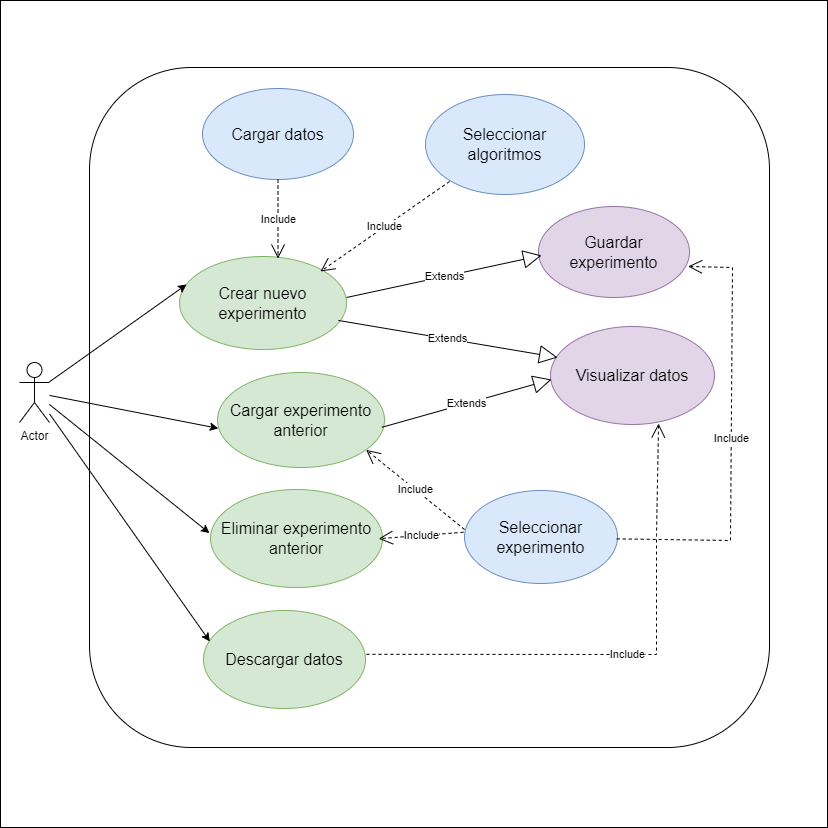
\includegraphics[width=1\linewidth]{img/Diagrama_CDU.png}
    \caption{Diagrama de casos de uso.}
    \label{Diagrama de casos de uso}
\end{figure}

En la ejecución del programa, el actor tiene tres acciones posibles: crear, cargar y descargar un experimento.

La creación de un nuevo experimento requiere que el usuario seleccione los algoritmos y los datos que se van a utilizar, lo cual incluye el paso de cargar los datos. Una vez realizados estos pasos, el nuevo experimento se guarda automáticamente y el usuario es llevado al apartado de visualización de datos.

Para cargar un experimento anterior, debe existir un experimento guardado previamente; en caso contrario, la selección del experimento (necesaria para este proceso) no será posible. Tras cargar el experimento, al igual que en la creación de uno nuevo, el usuario es dirigido al apartado de visualización de datos.

Finalmente, la descarga de un experimento solo será posible si el usuario se encuentra en el apartado de visualización, desde donde el programa permitirá realizar esta acción.

En conjunto, el sistema asegura un flujo coherente de acciones, permitiendo al usuario gestionar experimentos mediante la creación, carga, visualización y descarga de datos.

A continuación se mostrarán las tablas de uso:

\begin{table}[p]
	\centering
	\begin{tabularx}{\linewidth}{ p{0.21\columnwidth} p{0.71\columnwidth} }
		\toprule
		\textbf{CU-1}    & \textbf{Crear un nuevo experimento} \\
		\toprule
		\textbf{Versión}              & 1.0    \\
		\textbf{Autor}                & Álvaro González Delgado \\ 
		\textbf{Requisitos asociados} & RF-1, RF-2, RF-3 \\
		\textbf{Descripción}          & El usuario crea un nuevo experimento seleccionando los algoritmos y los datos que se van a usar. Los datos se cargan automáticamente, y el experimento se guarda en el sistema. El usuario es dirigido a la página de visualización de datos. \\
		\textbf{Precondición}         & El sistema debe permitir crear un nuevo experimento, no debe haber restricciones previas. Se debe haber seleccionado como mínimo un experimento y rellenado sus datos. El usuario deba haber introducido un conjunto de datos balido. \\
		
		\textbf{Acciones}             &
		\begin{enumerate}
			\item El usuario accede a la página de creación de un experimento.
			\item Elige los algoritmos y variables a utilizar.
			\item Se acede a la pagina de carga de datos.
			\item Se da un nombre Y se introducen los datos.
			\item Se carga los datos.
			\item Se ejecuta el algoritmo TRA-ClUS con todas las variables introducidas.
			\item Se finaliza la carga del algoritmo.
			\item El sistema guarda el experimento automáticamente.
			\item El sistema redirige al usuario a la página de visualización de datos.
		\end{enumerate} \\
		\textbf{Postcondición}        & El experimento es guardado en el sistema y se presenta la página de visualización de datos. \\
		\textbf{Excepciones}          & Si los datos seleccionados no dan un resultado valido o hay un error de conexión el sistema muestra un error. \\
		\textbf{Importancia}          & Alta \\
		\bottomrule
	\end{tabularx}
	\caption{CU-1 Crear un nuevo experimento.}
\end{table}

\FloatBarrier

\begin{table}[p]
	\centering
	\begin{tabularx}{\linewidth}{ p{0.21\columnwidth} p{0.71\columnwidth} }
		\toprule
		\textbf{CU-2}    & \textbf{Cargar un experimento existente} \\
		\toprule
		\textbf{Versión}              & 1.0    \\
		\textbf{Autor}                & Álvaro González Delgado \\
		\textbf{Requisitos asociados} & RF-1, RF-2 \\
		\textbf{Descripción}          & El usuario carga un experimento previamente guardado. El sistema permite seleccionar un experimento de la lista disponible y lo carga para continuar con el análisis. \\
		\textbf{Precondición}         & Debe existir al menos un experimento previamente guardado. \\
		\textbf{Acciones}             &
		\begin{enumerate}
			\item El usuario elige el experimento de la lista de experimentos guardados.
			\item El sistema carga el experimento y presenta la página de visualización de datos.
		\end{enumerate} \\
		\textbf{Postcondición}        & El experimento cargado se muestra en la página de visualización de datos. \\
		\textbf{Excepciones}          & Si no existen experimentos guardados, el sistema nuestra el desplegable vació y no puede seleccionarse nada. \\
		\textbf{Importancia}          & Alta \\
		\bottomrule
	\end{tabularx}
	\caption{CU-2 Cargar un experimento existente.}
\end{table}

\FloatBarrier

\begin{table}[p]
	\centering
	\begin{tabularx}{\linewidth}{ p{0.21\columnwidth} p{0.71\columnwidth} }
		\toprule
		\textbf{CU-3}    & \textbf{Descargar los resultados de un experimento} \\
		\toprule
		\textbf{Versión}              & 1.0    \\
		\textbf{Autor}                & Álvaro González Delgado \\
		\textbf{Requisitos asociados} & RF-4 \\
		\textbf{Descripción}          & El usuario puede descargar los resultados generados por el algoritmo TRA-CLUS en formato .zip. \\
		\textbf{Precondición}         & El usuario debe estar en una de las páginas de visualización de datos. \\
		\textbf{Acciones}             &
		\begin{enumerate}
			\item El usuario accede a la página de visualización de datos cargando un experimento nuevo o guardado.
			\item El usuario presiona el botón de descarga.
			\item El sistema descarga los resultados en el formato .zip.
		\end{enumerate} \\
		\textbf{Postcondición}        & Los resultados se descargan correctamente al dispositivo del usuario. \\
		\textbf{Excepciones}          & Si no hay resultados disponibles para descargar, el sistema no hace nada. \\
		\textbf{Importancia}          & Media \\
		\bottomrule
	\end{tabularx}
	\caption{CU-3 Descargar los resultados de un experimento.}
\end{table}

\FloatBarrier

\begin{table}[p]
	\centering
	\begin{tabularx}{\linewidth}{ p{0.21\columnwidth} p{0.71\columnwidth} }
		\toprule
		\textbf{CU-4}    & \textbf{Borrar un experimento existente} \\
		\toprule
		\textbf{Versión}              & 1.0    \\
		\textbf{Autor}                & Alumno \\
		\textbf{Requisitos asociados} & RF-5 \\
		\textbf{Descripción}          & El usuario puede borrar un experimento previamente guardado. La eliminación es irreversible. \\
		\textbf{Precondición}         & El experimento debe existir previamente. \\
		\textbf{Acciones}             &
		\begin{enumerate}
			\item El usuario elige el experimento que desea borrar de la lista.
			\item El sistema despliega la petición de confirmación.
			\item El sistema elimina el experimento y confirma la eliminación.
		\end{enumerate} \\
		\textbf{Postcondición}        & El experimento es eliminado del sistema de forma irreversible. \\
		\textbf{Excepciones}          & Si el experimento no existe, el botón no racionara. \\
		\textbf{Importancia}          & Media \\
		\bottomrule
	\end{tabularx}
	\caption{CU-4 Borrar un experimento existente.}
\end{table}

\FloatBarrier
\apendice{Especificación de diseño}

\section{Introducción}



\section{Diseño de datos}



\section{Diseño procedimental}



\section{Diseño arquitectónico}





\apendice{Documentación técnica de programación}

\section{Introducción}

En este apéndice se presenta la documentación técnica del proyecto, proporcionando una descripción detallada de la estructura del código y sus directorios. Este apartado tiene como objetivo facilitar la comprensión del proyecto para desarrolladores que deseen trabajar en él, analizarlo o realizar modificaciones futuras.

\section{Estructura de directorios}

Todo el código de este proyecto se encuentra dentro de la carpeta \texttt{code}, que se divide en dos subcarpetas principales:

\begin{itemize}
    \item \texttt{app/} -- Contiene toda la aplicación web desarrollada para el proyecto, organizada siguiendo el patrón Modelo-Vista-Controlador (MVC). Incluye el código relacionado con los controladores, modelos, vistas y utilidades, así como los recursos estáticos necesarios para la interfaz de usuario.
    \item \texttt{Research and experiments/} -- Agrupa todas las pruebas y experimentos realizados durante el desarrollo. En esta carpeta se incluyen tanto los prototipos iniciales como los análisis realizados con diferentes componentes del proyecto. Solo se han conservado aquellas pruebas que se consideran claras y relevantes.
\end{itemize}

Además, la documentación generada durante el desarrollo se encuentra en la carpeta \texttt{docs/latex}.

A continuación, se describe la estructura interna en detalle, destacando las funcionalidades principales de cada archivo o directorio:

\subsection*{Estructura de la aplicación}
            
\begin{itemize}
    \item \texttt{code/}
    \begin{itemize}
        \item \texttt{app/} -- Directorio principal de la aplicación web.
        \item \texttt{Research and experiments/} -- Directorio que contiene experimentos y pruebas realizadas durante el desarrollo.
    \end{itemize}
\end{itemize}

\begin{itemize}
	\item \texttt{app/}
	\begin{itemize}
		\item \texttt{controllers/} -- Contiene la lógica principal de control que conecta los modelos con las vistas.
        	\begin{itemize}
        		\item \texttt{\_\_init\_\_.py} -- Archivo de inicialización del módulo.
        		\item \texttt{callbacks.py} -- Define los callbacks utilizados en la aplicación, gestionando la interacción entre la interfaz de usuario y la lógica del servidor.
        		\item \texttt{clustering.py} -- Implementa funciones relacionadas con la ejecución de algoritmos de agrupamiento, incluyendo TRACLUS.
 		\end{itemize}
        	\item \texttt{models/} -- Agrupa la lógica de procesamiento de datos y las funciones principales del algoritmo TRACLUS.
         \begin{itemize}
         	\item \texttt{\_\_init\_\_.py} -- Archivo de inicialización del módulo.
         	\item \texttt{data\_processing.py} -- Contiene funciones para la limpieza, transformación y preparación de los datos.
         	\item \texttt{mapping.py} -- Proporciona herramientas para la visualización de datos geoespaciales.
         	\item \texttt{TRACLUS.py} -- Implementa el núcleo del algoritmo TRACLUS.
		\end{itemize}
        	\item \texttt{saved\_results/} -- Almacena resultados generados y guardados por el usuario.
        	\item \texttt{test/} -- Contiene pruebas unitarias y funcionales.
        	\begin{itemize}
        		\item \texttt{\_\_init\_\_.py} -- Archivo de inicialización del módulo de pruebas.
        		\item \texttt{text\_callbacks.py} -- Pruebas específicas para los callbacks de la aplicación.
		\end{itemize}
        	\item \texttt{utils/} -- Incluye utilidades generales y configuraciones globales.
        	\begin{itemize}
        		\item \texttt{\_\_init\_\_.py} -- Archivo de inicialización del módulo.
         	\item \texttt{config.py} -- Configuraciones generales del proyecto, como rutas y parámetros predeterminados.
        		\item \texttt{data\_utils.py} -- Funciones auxiliares para manipulación de datos.
        	\end{itemize}
        	\item \texttt{views/} -- Directorio que agrupa las vistas y la estructura visual de la aplicación.
 		\begin{itemize}
        		\item \texttt{assets/} -- Contiene recursos estáticos como hojas de estilo y archivos multimedia.
			\begin{itemize}
            		\item \texttt{style.css} -- Archivo CSS para la personalización del diseño de la interfaz de usuario.
            	\end{itemize}
			\item \texttt{layout/} -- Define las vistas de cada sección de la aplicación.
			\begin{itemize}
            		\item \texttt{\_\_init\_\_.py} -- Archivo de inicialización del módulo.
           		\item \texttt{datauptate\_page.py} -- Página para la carga y actualización de datos.
            		\item \texttt{experiment\_page.py} -- Página para seleccionar algoritmos de clustering.
            		\item \texttt{map\_page.py} -- Página que muestra mapas con los datos sin tratar.
            		\item \texttt{select\_page.py} -- Página para la selección del experimento o la creación de uno nuevo.
            		\item \texttt{table\_page.py} -- Página para mostrar tablas con los resultados del análisis.
				\item \texttt{TRACLUSmap\_page.py} -- Página que muestra mapas con los resultados del algoritmo TRACLUS.
			\end{itemize}
		\end{itemize}
		\item \texttt{\_\_init\_\_.py} -- Archivo de inicialización del módulo principal.
		\item \texttt{main.py} -- Archivo principal que ejecuta la aplicación web.
		\item \texttt{requirements.txt} -- Archivo que especifica las dependencias necesarias para ejecutar el proyecto.
    \end{itemize}
\end{itemize}

\subsection*{Estructura de la documentación}

\begin{itemize}
    \item \texttt{img/} -- Imágenes utilizadas en la documentación.
    \item \texttt{tex/} -- Archivos \LaTeX{} para generar documentos técnicos.
    \item \texttt{README.md} -- Archivo con instrucciones generales del proyecto.
    \item \texttt{anexos.pdf} -- Documento de anexos generado.
    \item \texttt{anexos.tex} -- Código fuente del documento de anexos.
    \item \texttt{bibliografia.bib} -- Archivo BibTeX con referencias bibliográficas principales.
    \item \texttt{bibliografiaAnexos.bib} -- Archivo BibTeX con referencias adicionales.
    \item \texttt{memoria.pdf} -- Documento principal del proyecto.
    \item \texttt{memoria.tex} -- Código fuente del documento principal.
\end{itemize}


\section{Manual del programador}

Este apartado proporciona información sobre las herramientas clave que un programador necesita para trabajar en el proyecto de manera eficiente, desde la instalación hasta la configuración del entorno de desarrollo.

\subsection{Herramientas clave}

A continuación, se detallan las herramientas y su configuración:

\subsubsection{Git}
Git es esencial para gestionar el control de versiones del proyecto.

\begin{enumerate}
    \item Descargue e instale Git desde la página oficial: \url{https://git-scm.com/}.
    \item Configure su nombre de usuario y correo electrónico:
    \begin{verbatim}
    git config --global user.name "TuNombre"
    git config --global user.email "TuCorreo@example.com"
    \end{verbatim}
    \item Clone el repositorio del proyecto:
    \begin{verbatim}
    git clone https://github.com/agd1017/TFG_TRACLUS.git
    \end{verbatim}
\end{enumerate}

\subsubsection{Visual Studio Code}
Visual Studio Code es el editor recomendado.

\begin{enumerate}
    \item Descargue VS Code desde: \url{https://code.visualstudio.com/}.
    \item Instale las extensiones sugeridas:
    \begin{itemize}
        \item Python.
        \item Pylance.
        \item GitLens.
    \end{itemize}
    \item Configure el intérprete de Python para que apunte a su entorno virtual.
\end{enumerate}

\subsubsection{Python}
El proyecto requiere Python 3.11.2 o superior.

\begin{enumerate}
    \item Descargue Python desde: \url{https://www.python.org/}.
    \item Durante la instalación, habilite la opción \textit{Add Python to PATH}.
    \item Verifique la instalación con:
    \begin{verbatim}
    python --version
    \end{verbatim}
\end{enumerate}

\subsubsection{Librerías Python}
El archivo \texttt{requirements.txt} especifica las dependencias necesarias.

\begin{enumerate}
    \item Cree un entorno virtual:
    \begin{verbatim}
    python -m venv venv
    \end{verbatim}
    \item Active el entorno virtual:
    \begin{itemize}
        \item En Windows:
        \begin{verbatim}
        venv\Scripts\activate
        \end{verbatim}
        \item En macOS/Linux:
        \begin{verbatim}
        source venv/bin/activate
        \end{verbatim}
    \end{itemize}
    \item Instale las dependencias:
    \begin{verbatim}
    pip install -r requirements.txt
    \end{verbatim}
\end{enumerate}

\section{Compilación, instalación y ejecución del proyecto}

En este apartado se detallan los pasos para ejecutar el proyecto en un entorno local desde el código fuente.

\subsection{Preparación del entorno}
\begin{enumerate}
    \item Asegúrese de haber instalado todas las herramientas clave mencionadas en el \textit{Manual del programador}.
    \item Clone el repositorio del proyecto en su máquina local.
    \item Navegue hasta la carpeta \texttt{code/app}.
    \item Cree y active el entorno virtual como se describe en la sección de \texttt{Librerías Python}.
\end{enumerate}

\subsection{Ejecución del proyecto}
\begin{enumerate}
    \item Ejecute el archivo principal de la aplicación:
    \begin{verbatim}
    python main.py
    \end{verbatim}
    \item Abra un navegador web y acceda a:
    \begin{verbatim}
    http://127.0.0.1:8050/
    \end{verbatim}
\end{enumerate}

\subsection{Modificaciones y control de versiones}
Para realizar cambios en el código:
\begin{enumerate}
    \item Edite los archivos necesarios utilizando Visual Studio Code.
    \item Guarde los cambios y verifique que la aplicación funcione correctamente.
    \item Utilice Git para gestionar los cambios:
    \begin{verbatim}
    git add .
    git commit -m "Descripción de los cambios"
    git push origin rama-principal
    \end{verbatim}
\end{enumerate}

Con estas instrucciones, el programador podrá compilar, instalar y ejecutar el proyecto localmente de manera efectiva.

\section{Despliegue de la aplicación}

Para que la aplicación web funcionase correctamente y otros usuarios pudieran utilizarla, era necesario desplegarla desde el entorno local a un entorno de producción. Existen dos formas principales de realizar este proceso: crear un servidor propio o subir la aplicación a un servidor en la nube proporcionado por un tercero. Por razones económicas, se decidió optar por la segunda opción y utilizar un servidor en la nube. Para ello, se exploraron diversos servicios compatibles con aplicaciones basadas en Python.

Entre las opciones evaluadas se encontraron AWS, Azure, Heroku y Conduktor. Aunque muchas de estas plataformas ofrecían soluciones robustas con buen rendimiento, todas presentaban limitaciones económicas, ya que sus funcionalidades avanzadas suelen estar asociadas a costos recurrentes. Esto nos llevó a buscar servicios que ofrecieran una base gratuita que cubriese nuestras necesidades principales.

\subsection{Render: la solución elegida}

Tras evaluar diferentes opciones, se decidió utilizar \textbf{Render}, una plataforma que permite el despliegue de aplicaciones web, APIs y otros servicios. Render ofrece un plan gratuito que resulta ideal para proyectos pequeños o de desarrollo inicial, lo que lo convierte en una opción atractiva para aquellos con presupuestos limitados.

Render proporciona varias ventajas para aplicaciones como la nuestra:
\begin{itemize}
    \item \textbf{Compatibilidad con Python:} Es compatible con aplicaciones basadas en frameworks como Dash, Flask o Django.
    \item \textbf{Despliegue automático:} Permite integrar repositorios de GitHub o GitLab para desplegar automáticamente los cambios realizados en el código.
    \item \textbf{Certificados SSL gratuitos:} Render ofrece certificados de seguridad SSL para garantizar conexiones seguras.
    \item \textbf{Facilidad de configuración:} La plataforma cuenta con una interfaz intuitiva y bien documentada, lo que facilita el proceso de configuración incluso para usuarios con experiencia limitada en despliegues.
    \item \textbf{Soporte para aplicaciones persistentes:} Render soporta aplicaciones que requieren bases de datos o almacenamiento adicional, ideal para aplicaciones web interactivas.
\end{itemize}

\subsection{Proceso de despliegue en Render}

El despliegue de la aplicación en Render se realizó siguiendo los pasos descritos a continuación:

\begin{enumerate}
    \item \textbf{Preparación del repositorio:}
    \begin{itemize}
        \item El proyecto ya estaba alojado en un repositorio de GitHub, se incluyo un archivo \texttt{requirements.txt} que especifica las dependencias necesarias para ejecutar la aplicación.
    \end{itemize}

    \item \textbf{Creación del servicio en Render:}
    \begin{itemize}
        \item Se creó una cuenta gratuita en Render.
        \item Desde el panel de control, se seleccionó la opción \textit{"New Web Service"} y se vinculó el repositorio de GitHub al servicio.
    \end{itemize}

    \item \textbf{Configuración del entorno:}
    \begin{itemize}
        \item Se especificó el comando de inicio de la aplicación, como \texttt{python code/app/main.py}.
        \item Se configuraron las variables de entorno necesarias, como claves API o configuraciones específicas de la aplicación.
    \end{itemize}

    \item \textbf{Despliegue automático:}
    \begin{itemize}
        \item Render detectó automáticamente el contenido del repositorio y comenzó el proceso de construcción e implementación.
        \item Una vez finalizado el proceso, se asignó una URL pública para acceder a la aplicación.
    \end{itemize}

    \item \textbf{Pruebas en producción:}
    \begin{itemize}
        \item Se realizaron pruebas para verificar que todas las funcionalidades de la aplicación estuvieran operativas y que no existieran problemas relacionados con dependencias o configuración.
    \end{itemize}
\end{enumerate}

\subsection{Consideraciones finales}

Aunque Render fue una herramienta muy útil durante el desarrollo, especialmente por su facilidad de uso y la ausencia de necesidad de gestionar infraestructura propia, las limitaciones en capacidad de procesamiento y memoria debido al bajo presupuesto impidieron realizar pruebas significativas de la aplicación. Estas restricciones, derivadas del plan gratuito, afectaron el rendimiento al procesar grandes volúmenes de datos y al manejar operaciones intensivas.  

Para que la aplicación pueda ser probada y utilizada en todo su potencial, sería necesario aumentar considerablemente el presupuesto destinado a recursos de servidor, lo que permitiría un entorno de despliegue más robusto y acorde a los requisitos de la aplicación.

\section{Pruebas del sistema}

En esta sección se describirá cómo realizar pruebas en el sistema para comprobar que los cambios realizados se han implementado correctamente.

\subsection{Prueba manual}

Las pruebas más utilizadas en este proyecto, especialmente para verificar la ejecución del algoritmo y la funcionalidad general de la aplicación, son de tipo manual.

Para realizar las pruebas de manera correcta y en un entorno local, se recomienda modificar la función \texttt{app.run\_server()} ubicada al final del archivo \texttt{main.py}. 

Se deben realizar los siguientes ajustes:
\begin{itemize}
    \item Añadir el parámetro \texttt{debug=True}, lo que permitirá visualizar en la consola los errores o advertencias durante la ejecución.
    \item Configurar el servidor local especificando el host y el puerto. Por ejemplo:
    \begin{verbatim}
    app.run_server(debug=True, host='127.0.0.1', port=8050)
    \end{verbatim}
\end{itemize}

Después de realizar esta configuración, ejecute el archivo \texttt{main.py}. Se deberá acceder en un navegador web a la dirección \texttt{http://127.0.0.1:8050}. Si la aplicación se ha cargado correctamente, se mostrará la página inicial, desde la cual podrá navegar y utilizarla normalmente.

Para realizar cualquier prueba, siga el flujo de trabajo estándar de la aplicación para llegar al recurso que desea verificar. Por ejemplo:
\begin{itemize}
    \item Si el cambio realizado afecta a la visualización de los resultados tras cargar un experimento, intente acceder a uno de los experimentos ya creados. 
    \item Si el cambio afecta a la carga de datos, deberá crear nuevos experimentos, ya que los experimentos guardados anteriormente no reflejarán los cambios en la lógica de carga.
\end{itemize}

En caso de que no sea posible acceder a los experimentos guardados, asegúrese de que la configuración de rutas en el archivo \texttt{config.py} sea válida para su dispositivo. Si es necesario, actualice las rutas para que apunten correctamente a las ubicaciones de los datos y recursos requeridos.

Este método permite identificar errores directamente en el flujo de trabajo de la aplicación y verificar que los cambios realizados se comporten de manera esperada.

\subsection{Testing}

El proyecto también incluye pruebas automáticas que pueden ejecutarse para verificar la funcionalidad de diversos componentes. Estas pruebas están ubicadas en el directorio \texttt{test/}.

\subsubsection{Ejecución de pruebas}

Para ejecutar las pruebas existentes, siga estos pasos:
\begin{enumerate}
    \item Asegúrese de que todas las dependencias necesarias estén instaladas. Puede verificar esto ejecutando:
    \begin{verbatim}
    pip install -r requirements.txt
    \end{verbatim}
    \item Desde la terminal, navegue hasta el directorio raíz del proyecto donde se encuentra el archivo \texttt{main.py}.
    \item Ejecute las pruebas utilizando el siguiente comando:
    \begin{verbatim}
    pytest -v {nombre test}
    \end{verbatim}
    \item Si este no funcion use el siguiente: 
    \begin{verbatim}
    PYTHONPATH=code/app pytest -v code/app/test/{nombre test}
    \end{verbatim}
    \item Revise los resultados en la terminal. Si alguna prueba falla, se mostrará el motivo del fallo y la ubicación correspondiente en el código.
\end{enumerate}

\subsubsection{Creación de nuevas pruebas}

Si necesita añadir nuevas pruebas al sistema, siga estos pasos:
\begin{enumerate}
    \item Cree un nuevo archivo de prueba en el directorio \texttt{test/}. Por convención, los archivos de prueba deben comenzar con el prefijo \texttt{test\_}, por ejemplo: \texttt{test\_nueva\_funcionalidad.py}.
    \item Dentro del archivo, defina funciones que comiencen con el prefijo \texttt{test\_}, como en el siguiente ejemplo:
    \begin{verbatim}
    def test_nueva_funcionalidad():
        resultado = funcion_a_probar(parametros)
        assert resultado == valor_esperado
    \end{verbatim}
    \item Utilice las funciones de prueba para validar las salidas de las funciones o métodos que haya implementado. Asegúrese de cubrir casos de uso válidos, así como posibles errores o entradas no válidas.
    \item Ejecute nuevamente \texttt{pytest} para confirmar que todas las pruebas, incluidas las nuevas, se ejecutan correctamente.
\end{enumerate}

Al incluir nuevas pruebas, asegúrese de documentar el propósito de cada prueba dentro del archivo correspondiente. Esto ayudará a otros desarrolladores a comprender el objetivo y alcance de cada conjunto de pruebas.




\apendice{Documentación de usuario}

\section{Introducción}

\section{Requisitos de usuarios}

\section{Instalación}

\section{Manual del usuario}




\apendice{Resultados estudio}

\section{Introducción}

En este apartado se detallaran las pruebas realizadas durante el desarrollo de la aplicación para mostrar su funcion.

\section{Comparativa de algoritmos}

Tras la optimización del algoritmo pero antes de la implementación a la pagina web, se buscó comparar el funcionamiento y los resultados que podían proporcionar los diferentes algoritmos de clustering bajo condiciones relativamente equivalentes. Para ello, se utilizó la misma cantidad de datos: doscientas filas del archivo \texttt{Trayectorias Taxis} \cite{trayectorias_taxis}. Respecto a los parámetros necesarios para la ejecución de cada algoritmo, se intentó mantenerlos lo más estándar posible. Por ejemplo, en los casos en que era necesario especificar el número de clusters, se utilizó una aproximación basada en el resultado obtenido por OPTICS, ya que este algoritmo no requiere definir dicho parámetro. El resto de los parámetros se dejaron en los valores predeterminados que proporciona la biblioteca \texttt{scikit-learn}.

Aunque se probaron más algoritmos, solo cinco llegaron a la etapa final del desarrollo de la página web. Algunos, como \textbf{Birch}, no lograron producir resultados satisfactorios, aunque se considera que, con una adaptación más específica de los datos, podrían haber funcionado correctamente.

A continuación, se describen los resultados obtenidos para cada uno de los algoritmos seleccionados:

\begin{enumerate}

\item \textbf{OPTICS}:  
Este fue el primer algoritmo probado de manera intensiva, ya que era el utilizado por defecto en la implementación base. De las doscientas filas procesadas, se generaron un total de 2161 segmentos, que fueron agrupados en 106 clusters. Sin embargo, no todos los segmentos se utilizaron para la creación de los clusters; un total de 1354 segmentos fueron catalogados como "basura", lo que corresponde al 62.66\% de los datos. A continuación, se muestran los resultados en tres imágenes diferentes: la representación de los clusters, un histograma con la cantidad de trayectorias que forman cada cluster y la representación de trayectorias generadas por el algoritmo TRACLUS.

\begin{figure}[h!]
    \centering
    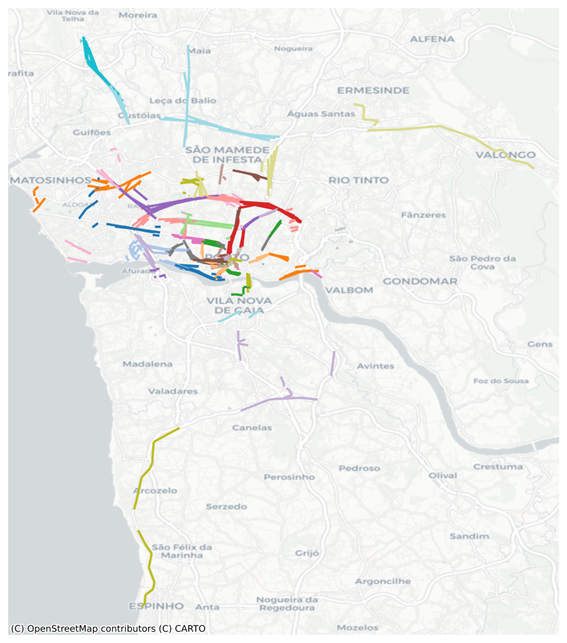
\includegraphics[width=0.5\textwidth]{img/clusters_OPTICS.png}
    \caption{Representación de clusters.}
    \label{fig:clusters_OPTICS}
\end{figure}

\begin{figure}[h!]
    \centering
    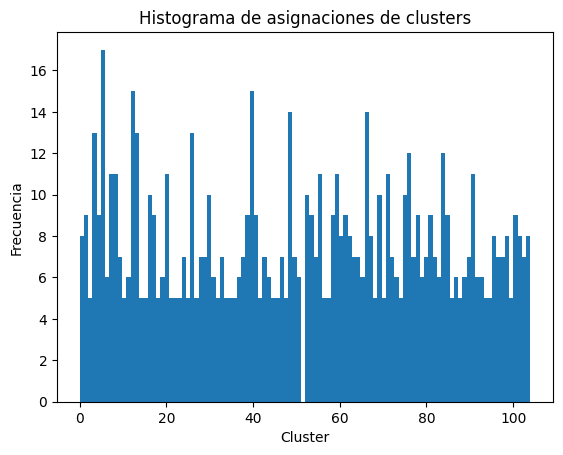
\includegraphics[width=0.5\textwidth]{img/histograma_OPTICS.png}
    \caption{Segmentos por cada cluster.}
    \label{fig:histograma_OPTICS}
\end{figure}

\begin{figure}[h!]
    \centering
    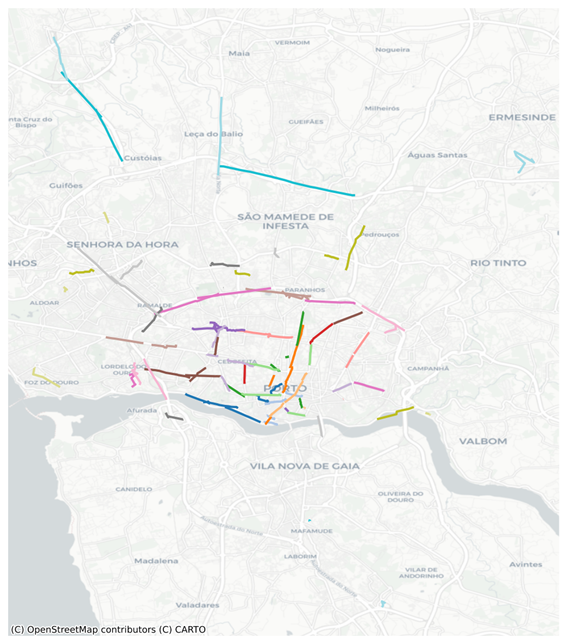
\includegraphics[width=0.5\textwidth]{img/r_tray_OPTICS.png}
    \caption{Representación de trayectorias.}
    \label{fig:trayectorias_OPTICS}
\end{figure}

\FloatBarrier

\item \textbf{DBSCAN}:  
Con un valor de \texttt{eps} de 0.1, los resultados de DBSCAN fueron significativamente diferentes a los de OPTICS. Aunque se generaron más segmentos (2654 en total), el número de clusters disminuyó a 37. Además, el porcentaje de datos clasificados como "basura" aumentó al 90.09\%, lo que equivale a 2391 segmentos descartados.

\begin{figure}[h!]
    \centering
    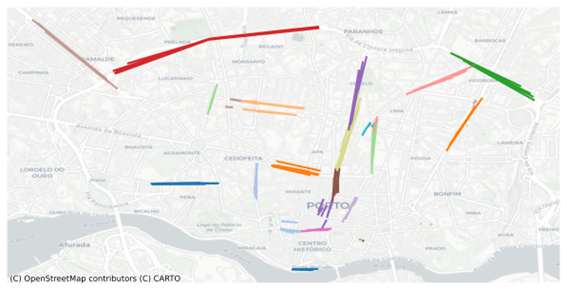
\includegraphics[width=0.5\textwidth]{img/clusters_DBSCAN.png}
    \caption{Representación de clusters.}
    \label{fig:clusters_DBSCAN}
\end{figure}

\begin{figure}[h!]
    \centering
    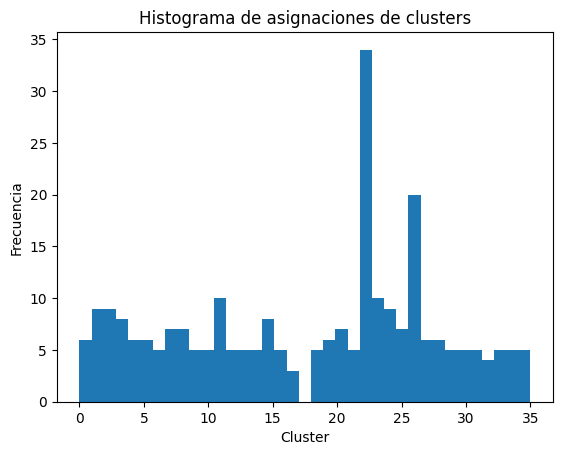
\includegraphics[width=0.5\textwidth]{img/histograma_DBSCAN.png}
    \caption{Segmentos por cada cluster.}
    \label{fig:histograma_DBSCAN}
\end{figure}

\begin{figure}[h!]
    \centering
    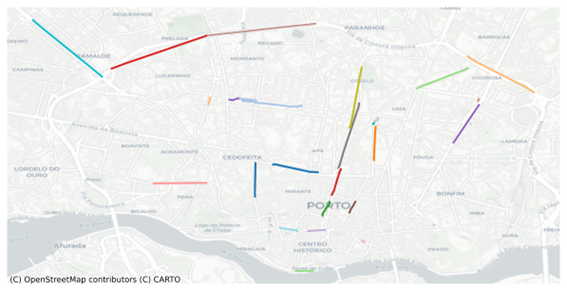
\includegraphics[width=0.5\textwidth]{img/r_tray_DBSCAN.png}
    \caption{Representación de trayectorias.}
    \label{fig:trayectorias_DBSCAN}
\end{figure}

\FloatBarrier

\item \textbf{HDBSCAN}:  
Este algoritmo no requirió ajustes en sus parámetros predeterminados de \texttt{scikit-learn}. Los resultados fueron similares a los de OPTICS en términos de segmentos (2161), aunque el número de clusters fue menor (96) y el porcentaje de segmentos descartados también disminuyó, alcanzando un 53.54\% (1157 segmentos).

\begin{figure}[h!]
    \centering
    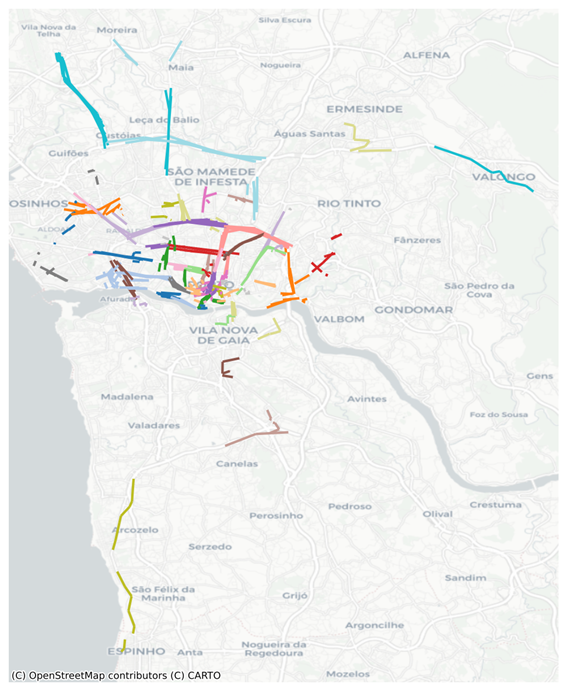
\includegraphics[width=0.5\textwidth]{img/clusters_HDBSCAN.png}
    \caption{Representación de clusters.}
    \label{fig:clusters_HDBSCAN}
\end{figure}

\begin{figure}[h!]
    \centering
    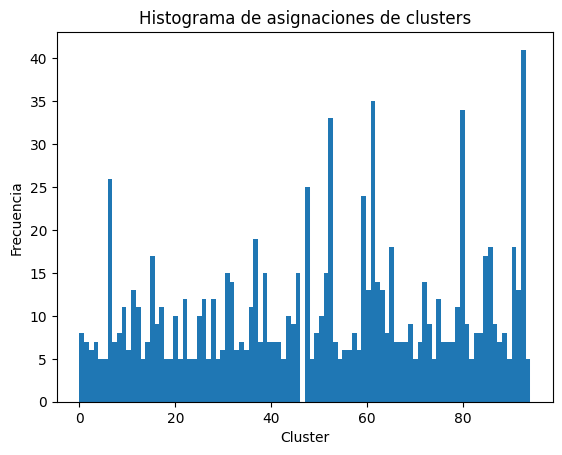
\includegraphics[width=0.5\textwidth]{img/histograma_HDBSCAN.png}
    \caption{Segmentos por cada cluster.}
    \label{fig:histograma_HDBSCAN}
\end{figure}

\begin{figure}[h!]
    \centering
    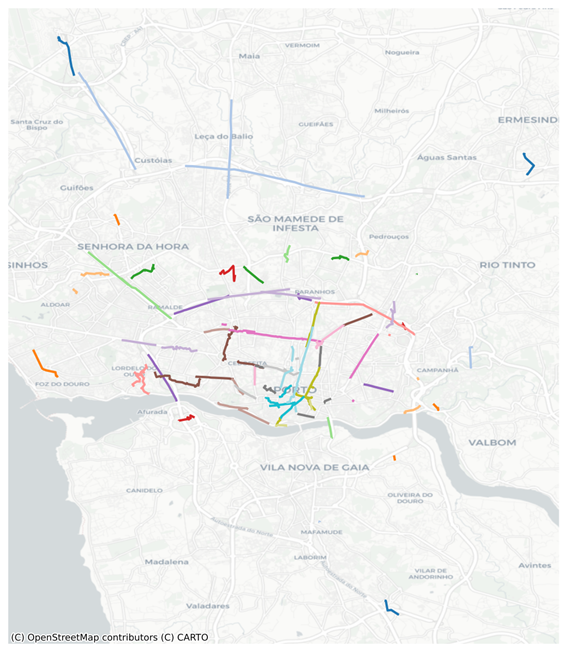
\includegraphics[width=0.5\textwidth]{img/r_tray_HDBSCAN.png}
    \caption{Representación de trayectorias.}
    \label{fig:trayectorias_HDBSCAN}
\end{figure}

\FloatBarrier

\item \textbf{Agglomerative Clustering}:  
Este algoritmo requería definir previamente el número de clusters. En este caso, se utilizaron los 2654 segmentos generados, sin descartar ninguno, ya que no clasifica datos como "basura". Sin embargo, esta característica provoca que los clusters no se centren en las zonas más densas, lo que resulta en representaciones de trayectorias más erráticas.

\begin{figure}[h!]
    \centering
    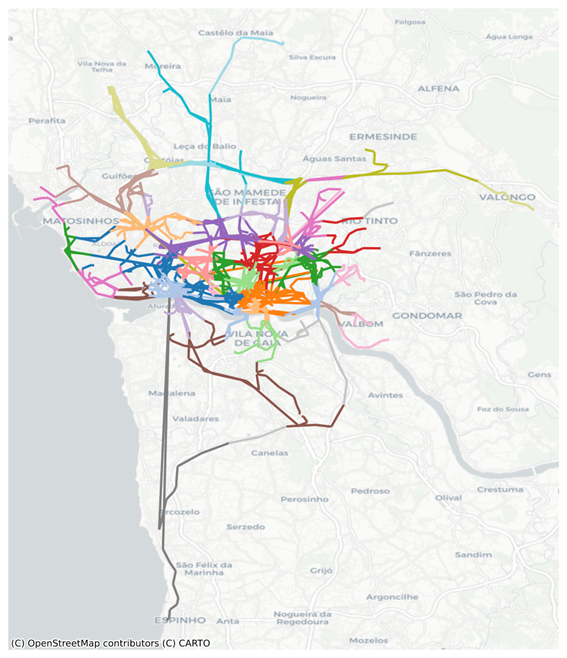
\includegraphics[width=0.5\textwidth]{img/clusters_Aggl.png}
    \caption{Representación de clusters.}
    \label{fig:clusters_Agglomerative}
\end{figure}

\begin{figure}[h!]
    \centering
    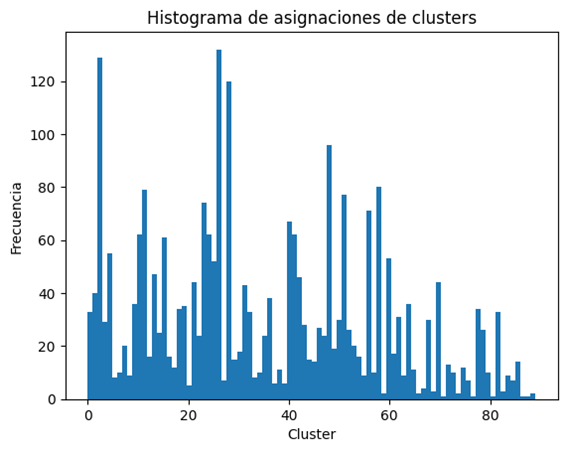
\includegraphics[width=0.5\textwidth]{img/histograma_Aggl.png}
    \caption{Segmentos por cada cluster.}
    \label{fig:histograma_Agglomerative}
\end{figure}

\begin{figure}[h!]
    \centering
    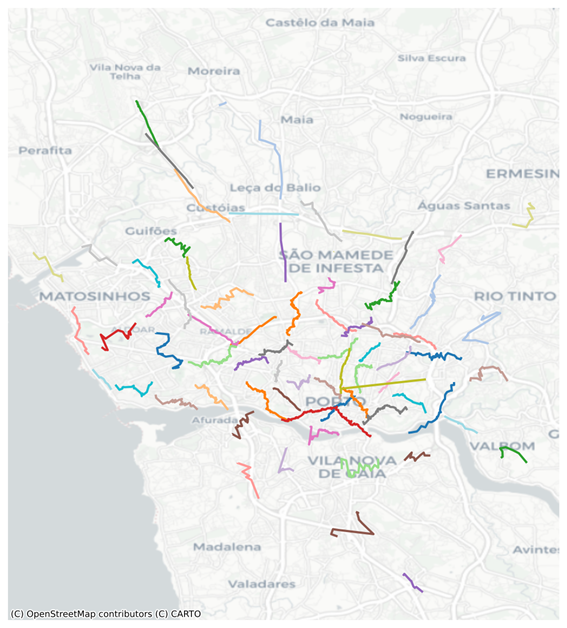
\includegraphics[width=0.5\textwidth]{img/r_tray_Aggl.png}
    \caption{Representación de trayectorias.}
    \label{fig:trayectorias_Agglomerative}
\end{figure}

\FloatBarrier

\item \textbf{Spectral Clustering}:  
Al igual que el algoritmo anterior, no descarta datos. Aunque se generaron los mismos 2654 segmentos y clusters que en Agglomerative Clustering, los resultados finales fueron diferentes, con una distribución menos centralizada.

\begin{figure}[h!]
    \centering
    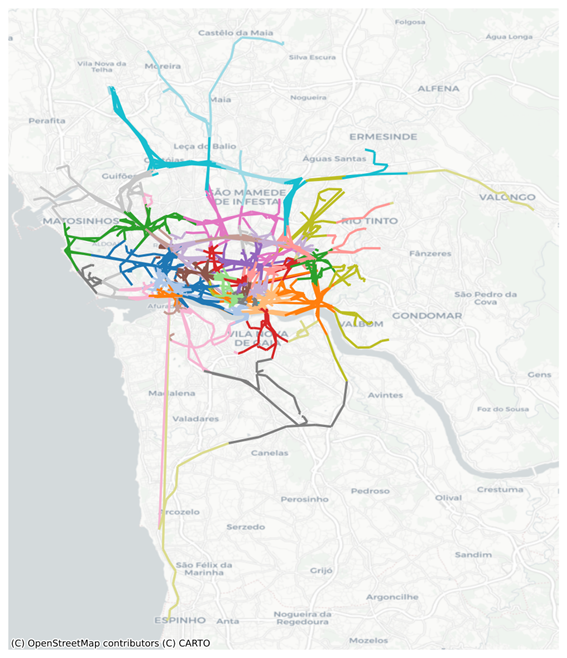
\includegraphics[width=0.5\textwidth]{img/clusters_Spect.png}
    \caption{Representación de clusters.}
    \label{fig:clusters_Spectral}
\end{figure}

\begin{figure}[h!]
    \centering
    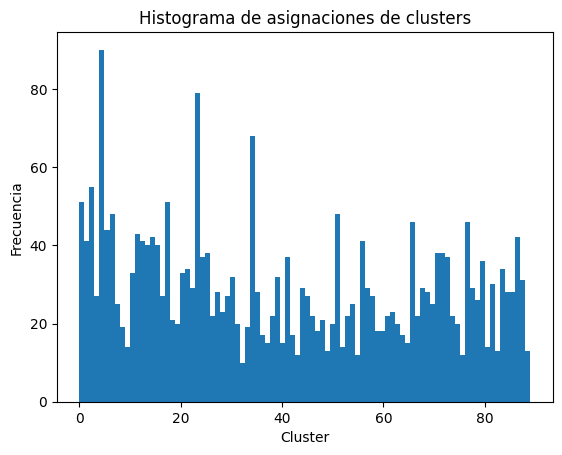
\includegraphics[width=0.5\textwidth]{img/histograma_Spect.png}
    \caption{Segmentos por cada cluster.}
    \label{fig:histograma_Spectral}
\end{figure}

\begin{figure}[h!]
    \centering
    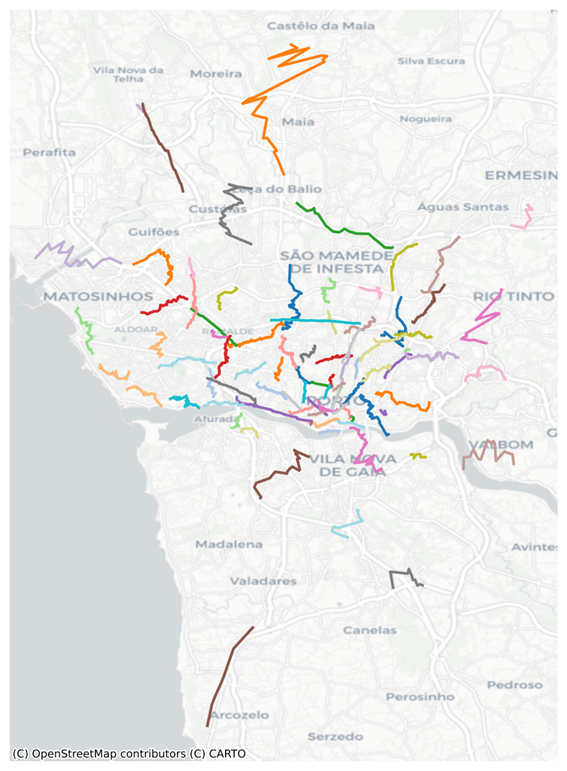
\includegraphics[width=0.5\textwidth]{img/r_tray_Spect.png}
    \caption{Representación de trayectorias.}
    \label{fig:trayectorias_Spectral}
\end{figure}

\FloatBarrier

\end{enumerate}

\subsection{Conclusión}

La comparativa de algoritmos de \textit{clustering} mostró diferencias significativas en los resultados obtenidos, claramente visibles en las imágenes de los clusters generados. Aunque se utilizó un conjunto de datos con 200 filas, aumentar la cantidad de datos podría mejorar la robustez de los resultados y proporcionar patrones más generalizables. En esta evaluación, \textbf{Spectral Clustering} y \textbf{Agglomerative Clustering} carecieron de configuraciones de parámetros que generaran clusters bien definidos, lo que resultó en trayectorias dispersas y difíciles de analizar. Por el contrario, \textbf{OPTICS} y \textbf{HDBSCAN} produjeron resultados más consistentes, siendo HDBSCAN el que clasificó un menor porcentaje de segmentos como "basura".

\textbf{DBSCAN} mostró una tendencia hacia rutas centralizadas, aunque con una tasa alta de segmentos descartados. Esto sugiere que DBSCAN podría ser más efectivo para identificar trayectorias centrales claras, aunque a costa de una menor utilización de datos. La elección del algoritmo más adecuado dependerá del contexto específico y de la importancia relativa de la densidad frente a la centralización de las rutas.

\begin{table}[ht]
\centering
\begin{tabular}{|l|c|c|c|}
\hline
\textbf{Algoritmo} & \textbf{Segmentos} & \textbf{Segmentos 'basura'} & \textbf{Clusters}  \\
\hline
OPTICS & 2161 & 62.66\% & 106 \\
DBSCAN & 2654 & 90.09\% & 37 \\
HDBSCAN & 2161 & 53.54\% & 96 \\
Spectral Clustering & 2654 & 0\% & 90 \\
Agglomerative Clustering & 2654 & 0\% & 90 \\
\hline
\end{tabular}
\caption{Resumen de resultados de los algoritmos de clustering}
\label{tabla:comparacion_algoritmos}
\end{table}



\section{Pruebas funcionales}

Para demostrar la utilidad del algoritmo y la aplicación creados, se propuso realizar múltiples pruebas con diferentes conjuntos de datos, tamaños y configuraciones aplicados a los algoritmos de clustering.

\subsection{Conjuntos de datos}

Durante el desarrollo del proyecto, se utilizó en prácticamente todo el conjunto de datos de Trayectorias Taxis \cite{trayectorias_taxis}. Para esta comprobación final, esto no era suficiente. Usar solo este conjunto de datos limitaría el proyecto a un análisis específico. Por lo tanto, se buscó encontrar múltiples conjuntos de datos.

Aunque existen multitud de conjuntos de datos con coordenadas GPS que pueden servir la mayoría de ellos no se encuentran en un formato preparado para correr el TRACLUS. Normalmente los conjuntos suelen separar las coordenadas en puntos lo cual no es valido ya que el TRACLUS, este necesita de trayectorias por tanto hay que juntar los datos de forma lógica con un formato valido. 

El primer conjunto con esa estructura adaptada fue Geolife \cite{geolife_trajectories}. Este estudio organiza los datos en carpetas, una por cada sujeto al que se le registraron ubicaciones durante un periodo de tiempo. Dentro de cada carpeta se encontraban varios archivos \texttt{.plt} que contenían información sobre la latitud, longitud, hora y fecha de las mediciones. 

Para organizar los datos de forma lógica para el algoritmo TRACLUS, no era viable crear una fila por cada archivo \texttt{.plt}, ya que algunos contenían más de 1000 mediciones. Por lo tanto, se decidió agrupar las mediciones por hora. Todas las mediciones tomadas dentro de la misma hora se combinaron en una única fila de un archivo Excel.

Se creó una función para automatizar este proceso por carpeta, lo que permitió realizar pruebas fácilmente en diferentes sujetos. Para analizar los resultados, se utilizó un archivo Excel generado con todos los datos encontrados en la carpeta del sujeto \texttt{000}.

Otro conjunto de datos probado fue uno de MoveBank \cite{movebank}, una plataforma que contiene miles de trayectorias de animales. Debido a la inmensidad de opciones disponibles, se seleccionó de forma semi-aleatoria el conjunto de datos titulado \textit{"Hammer-headed fruit bats (Hypsignathus monstrosus) in the Republic of Congo"}. Este conjunto incluía datos de múltiples murciélagos de la fruta registrados en diferentes días. 

Tras analizar el número de mediciones por hora, se decidió dividir las trayectorias por murciélago y día, creando un conjunto de datos con filas más reducidas en comparación al anterior. Aun así, estas filas eran considerablemente más grandes que las del conjunto de Trayectorias Taxis, lo cual incrementó significativamente el tiempo de procesamiento por cada fila analizada.

Ademas de estos tres se hicieron pruebas con otros como Citi Bikes \cite{citybike} o Foursquare-NY \cite{foursquare} pero los resultado no fueron visualmente atractivos para un buen analisis y muestra.

\subsection{Criterios para las pruebas:}

\begin{enumerate}
    \item \textbf{Límite de tiempo:} Cada prueba debe durar un máximo de dos horas, considerando tanto el tiempo de ejecución como el de representación de los datos. Este límite puede variar según el tamaño del conjunto de datos y el número de coordenadas procesadas.
    \item \textbf{Selección de parámetros:} No se probarán todas las combinaciones posibles. Se seleccionarán aquellas configuraciones que se consideren más relevantes y que puedan producir cambios significativos en los resultados.
    \item \textbf{Parámetros predeterminados:} En las pruebas que uno de los elementos se cambie el resto de ellos permanecerán con los siguientes valores: 
    
    \begin{itemize}
    		\item \textbf{Metric:} \texttt{euclidean}
    		\item \textbf{Algorithm:} \texttt{auto}
    		\item \textbf{Min\_samples:} 5
   		\item \textbf{Max\_eps:} 1
    		\item \textbf{Eps:} 0.1
    		\item \textbf{Linkage:} \texttt{ward}
    		\item \textbf{Affinity:} \texttt{nearest\_neighbors}
    		\item \textbf{Assign\_labels:} \texttt{kmeans}
    		\item \textbf{n\_clusters:} 7
	\end{itemize}

\end{enumerate}

\subsection{Resultados}

\subsubsection{OPTICS, DBSCAN y HDBSCAN}

En las pruebas iniciales, se observó que, debido a las características de los datos seleccionados, los algoritmos OPTICS y HDBSCAN tendían a comportarse de manera similar, con la principal diferencia siendo el parámetro \texttt{Max\_eps}, esta se calcula internamente en HDBSCAN por lo que dependiendo de la cantidad de datos esta cambiara. Por otro lado, DBSCAN también podría reproducir resultados similares bajo configuraciones específicas del parámetro \texttt{eps}. 

Para comprender cómo los parámetros afectan el rendimiento de cada algoritmo, se realizaron pruebas aislando cada parámetro. Es decir, al modificar un parámetro, los demás permanecieron en sus valores predeterminados.

\paragraph{Métricas (\texttt{metric})}

Las métricas utilizadas para calcular las distancias entre puntos demostraron tener un impacto significativo en los resultados. Los hallazgos principales fueron los siguientes:

- \textbf{Métricas no funcionales}: Algunas métricas, como \texttt{l1} y \texttt{cosine}, no pudieron procesar correctamente los datos seleccionados, lo que resultó en errores o en agrupaciones inadecuadas, sin embargo con otras cantidades u otros parámetros estas si que dieron resultado.

- \textbf{Manhattan}: Esta métrica tendió a considerar todos los puntos como parte de un único clúster grande, resultando en una agrupación poco informativa. En el caso de las trayectorias, esto significó un único grupo, lo que limitó el análisis.

\begin{figure}[h!]
    \centering
    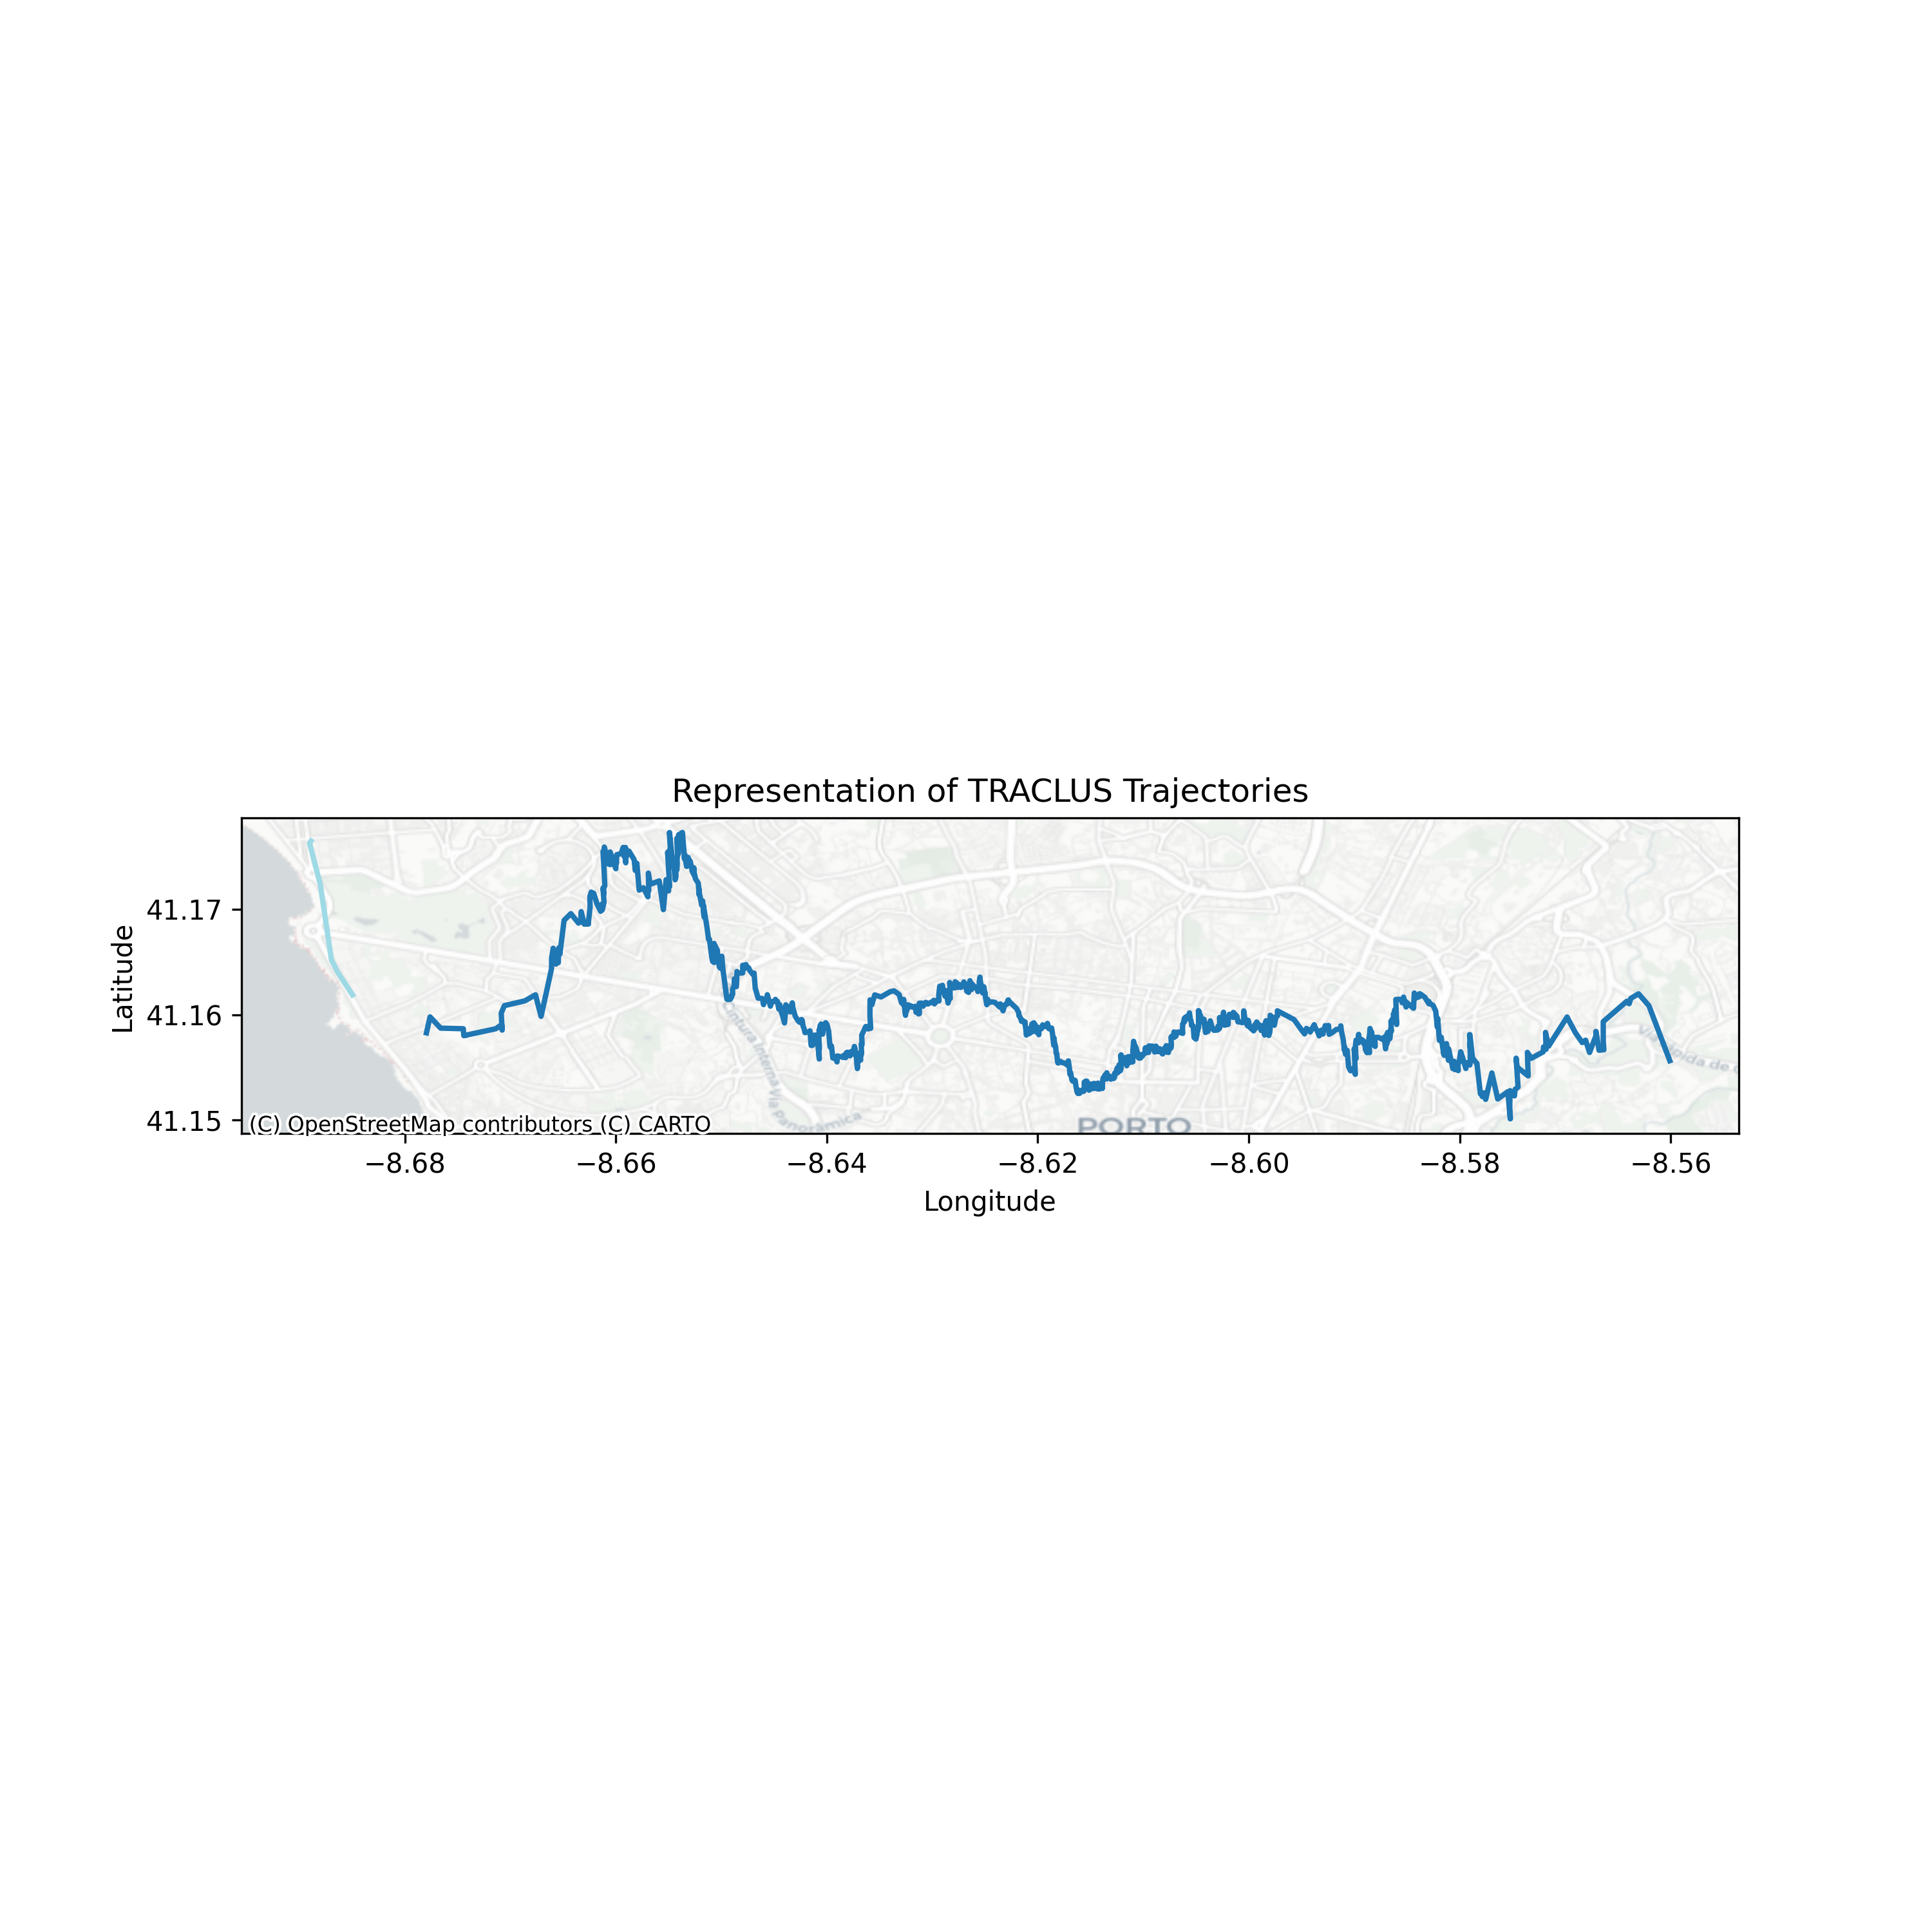
\includegraphics[width=0.8\textwidth]{img/Taxis/map_optics_manhatan.png}
    \caption{Resultados con la métrica Manhattan en OPTICS y HDBSCAN.}
    \label{fig:manhattan}
\end{figure}

\FloatBarrier

- \textbf{Euclidean y L2}: Ambas métricas ofrecieron resultados idénticos, creando agrupaciones claras y comprensibles. Estas métricas son particularmente adecuadas para este tipo de datos.

\begin{figure}[h!]
    \centering
    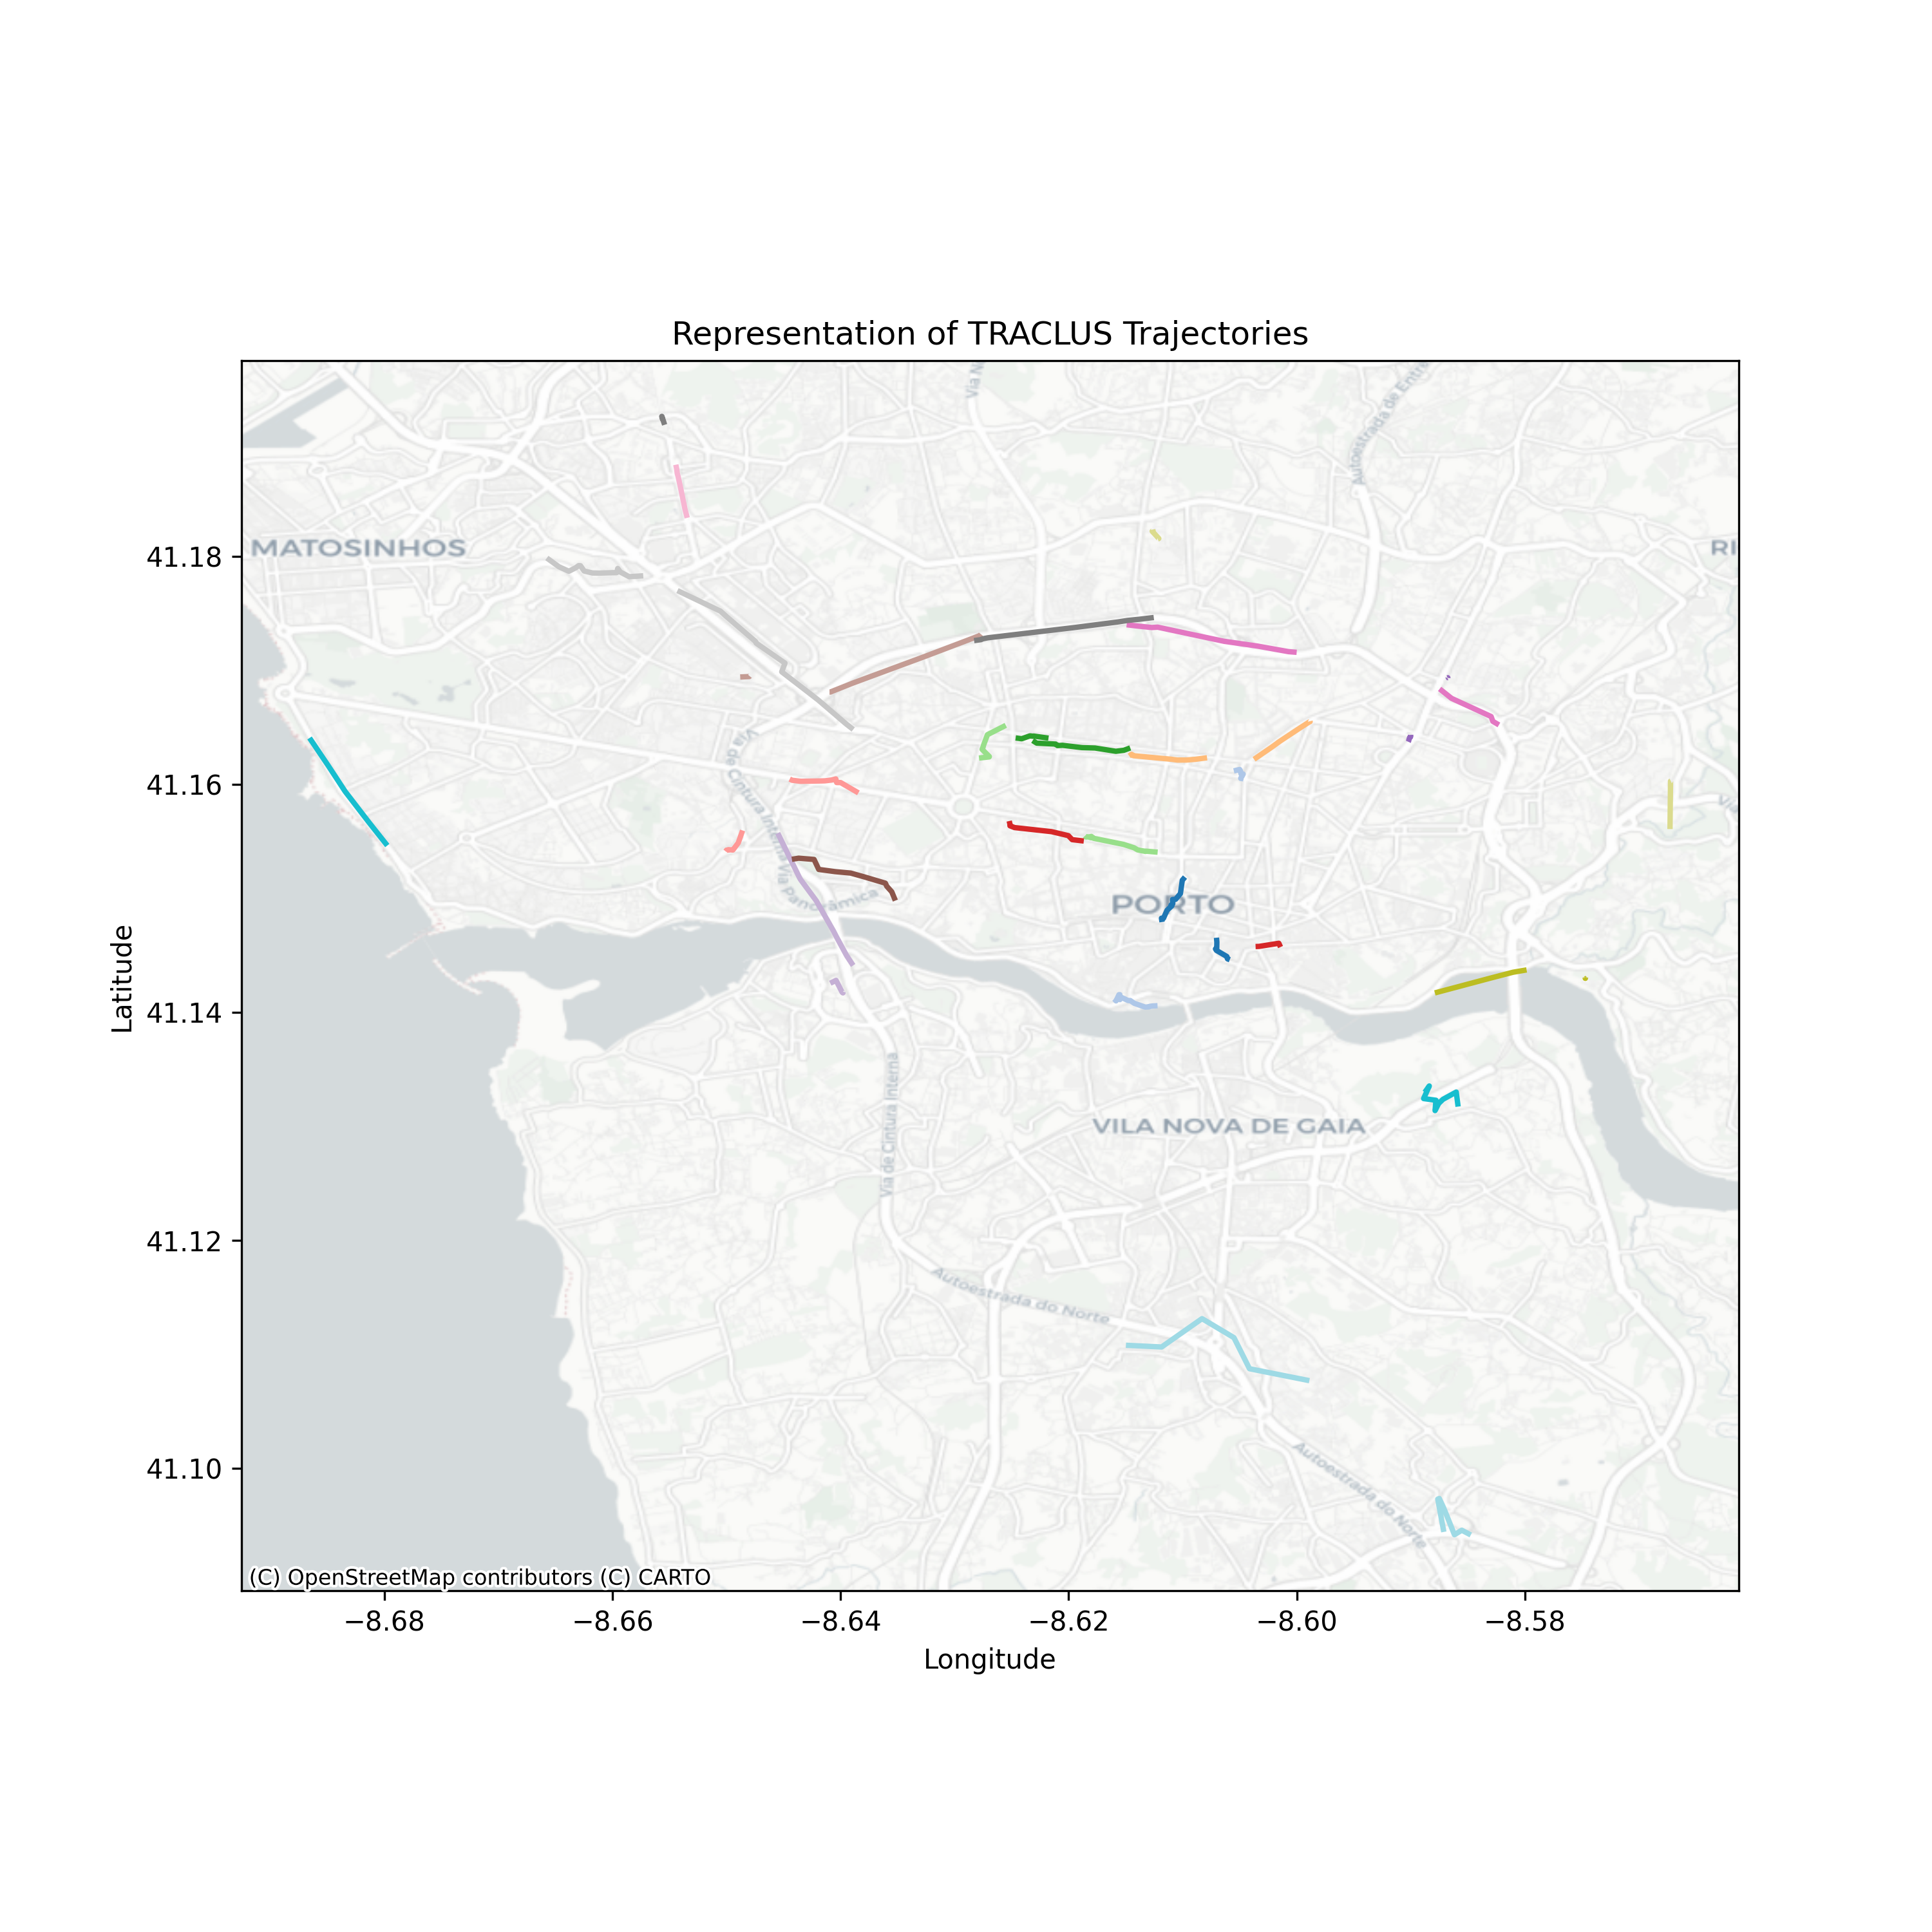
\includegraphics[width=0.8\textwidth]{img/Taxis/map_optics_l2.png}
    \caption{Resultados con las métricas Euclidean y L2 en OPTICS y HDBSCAN.}
    \label{fig:euclidean}
\end{figure}

\FloatBarrier

- \textbf{Cityblock}: Aunque mostró similitudes con las métricas anteriores, los clústeres resultantes eran menos definidos y algo más dispersos, lo que afectó la precisión de las trayectorias.

\begin{figure}[h!]
    \centering
    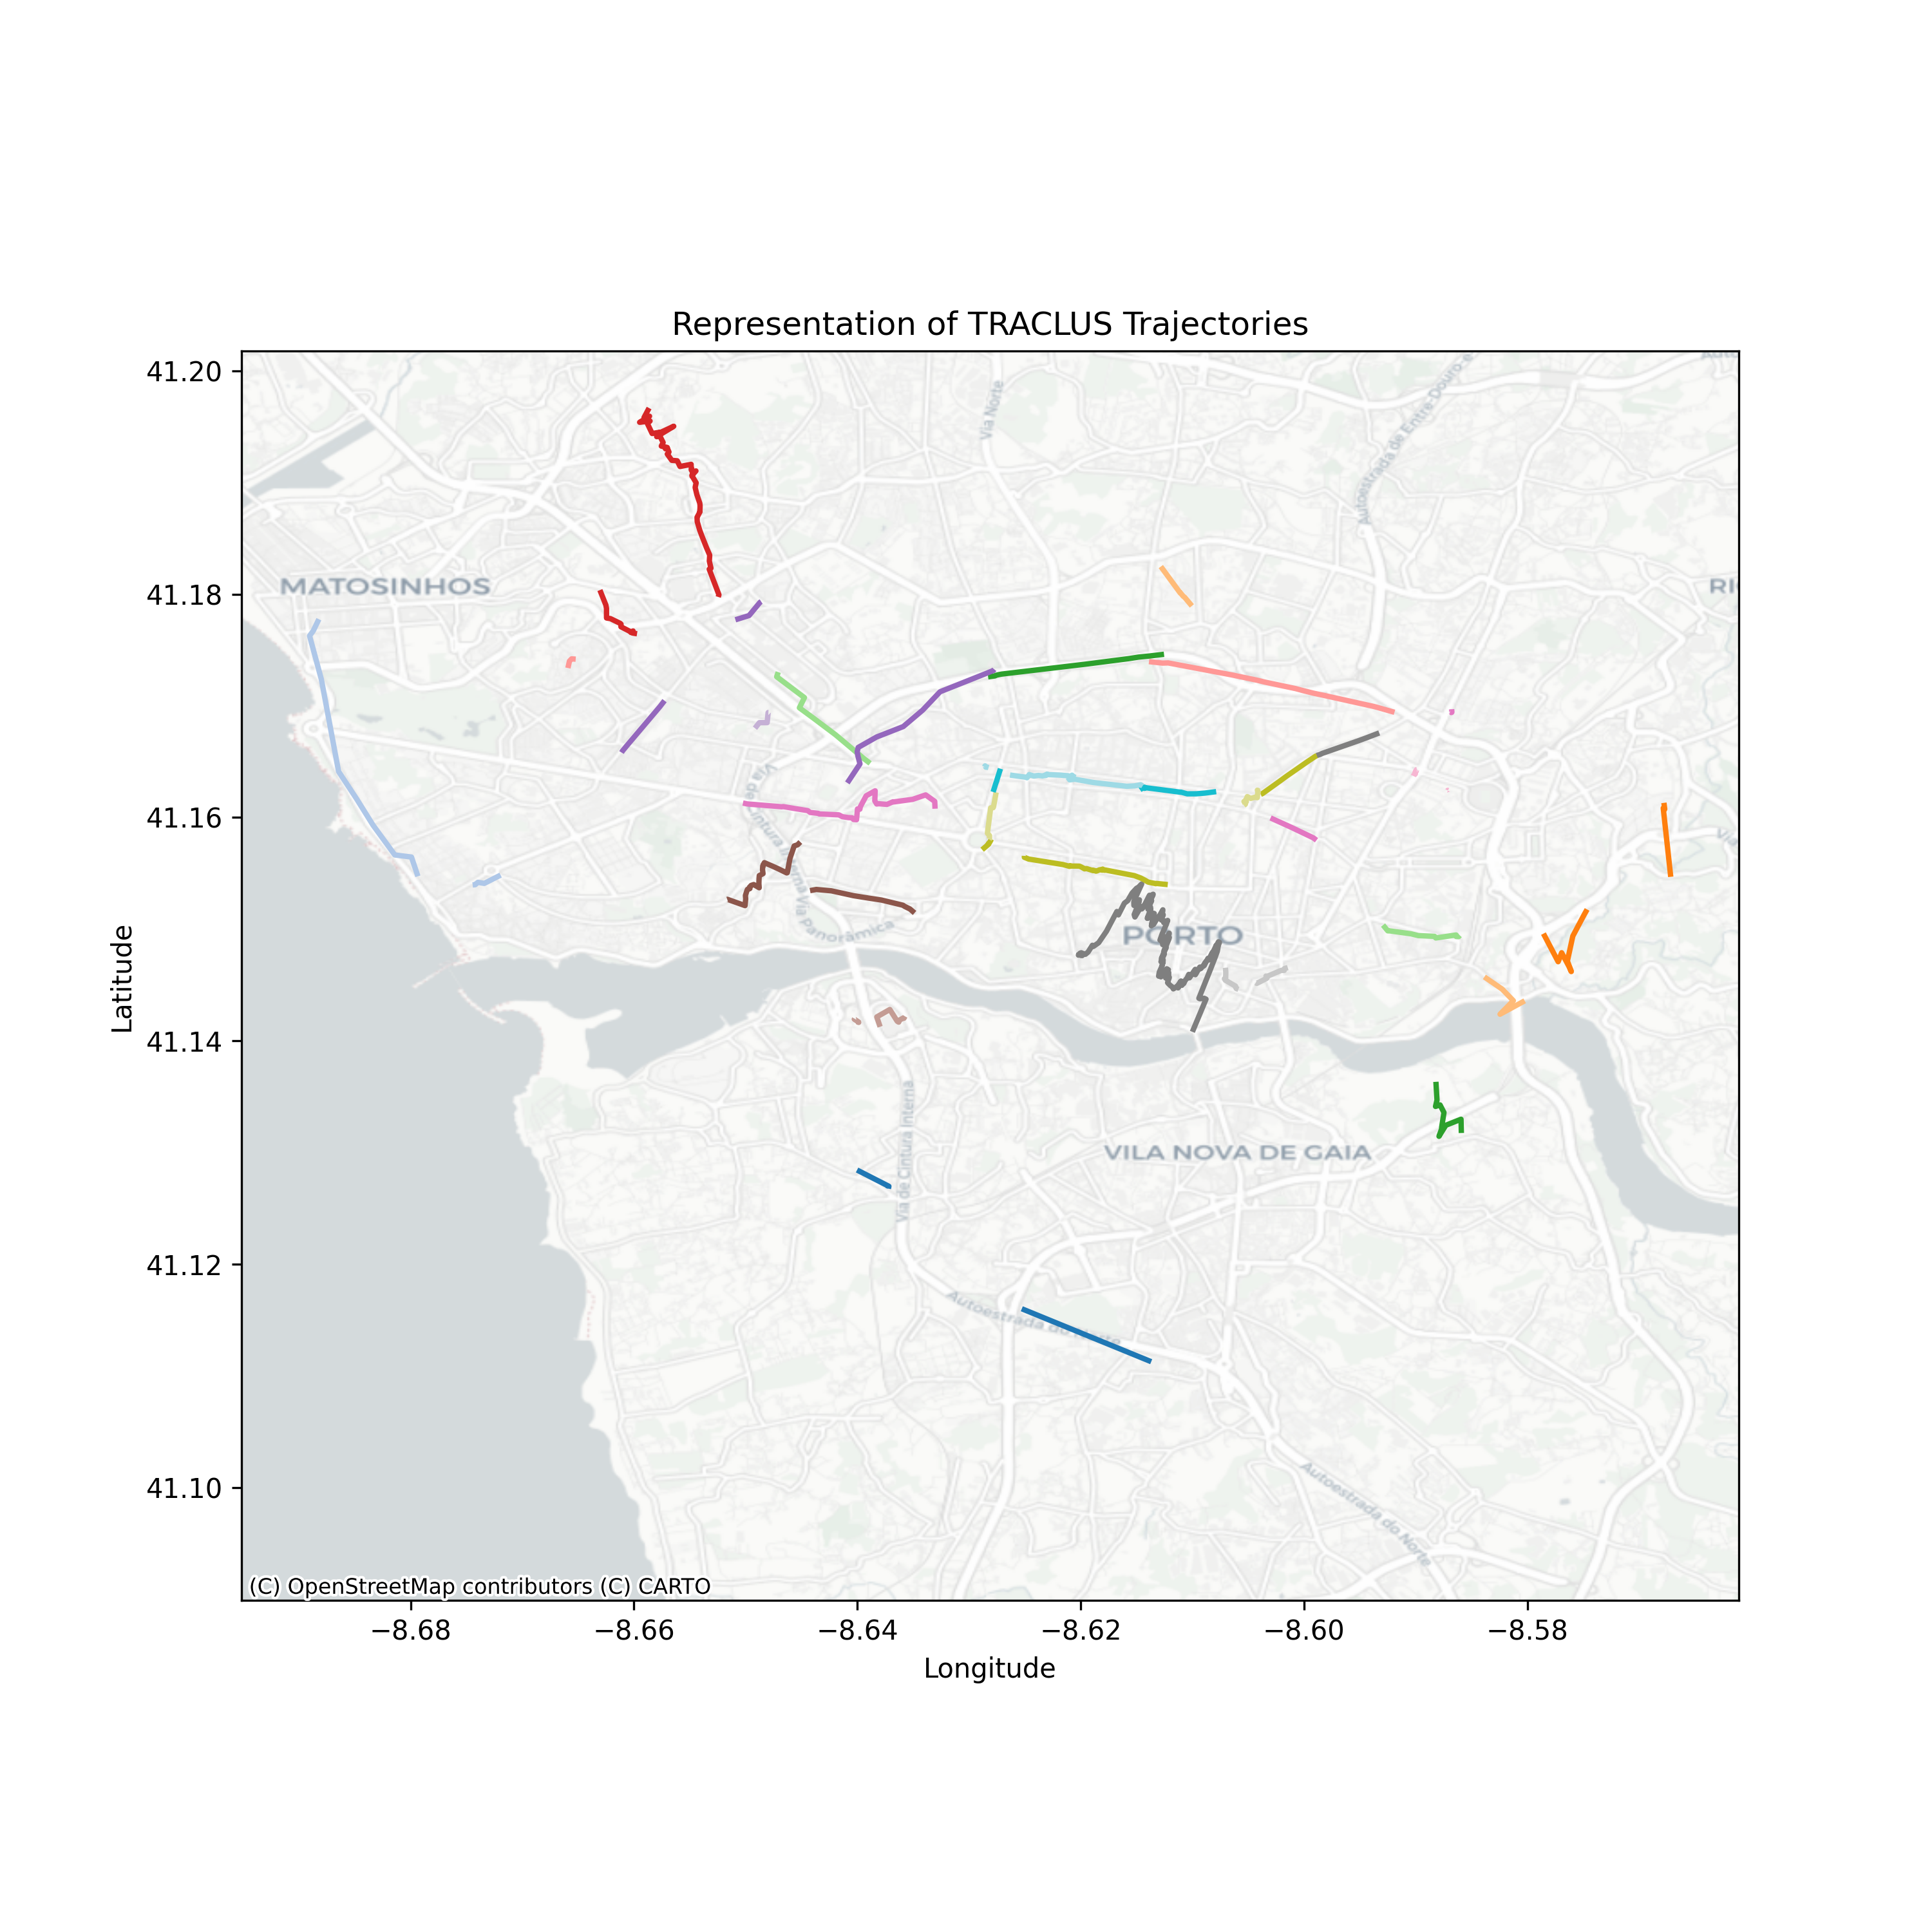
\includegraphics[width=0.8\textwidth]{img/Taxis/map_optics_city.png}
    \caption{Resultados con la métrica Cityblock en OPTICS y HDBSCAN.}
    \label{fig:cityblock}
\end{figure}

\FloatBarrier

En general, se determinó que el uso de métricas como Euclidean o L2 es más recomendable, mientras que Manhattan y otras métricas no lineales presentaron limitaciones significativas en este conjunto de datos. Sin embargo, esta conclusión no se pude aplicar en cambios de todos los parámetros.


\paragraph{Algoritmo (\texttt{algorithm})}

El parámetro \texttt{algorithm} define la estrategia interna utilizada por el algoritmo para calcular los clústeres. Los resultados variaron dependiendo del conjunto de datos empleado:

-\textbf{Trayectorias Taxis}:

A diferencia de las metricas que si se comportaban de la misma forma en los tres algoritmos, el parametro algoritmo variaba en gran mediada, para empezar, OPTICS no recibia cambios dando igual cual de ellas se probara.

\begin{figure}[h!]
    \centering
    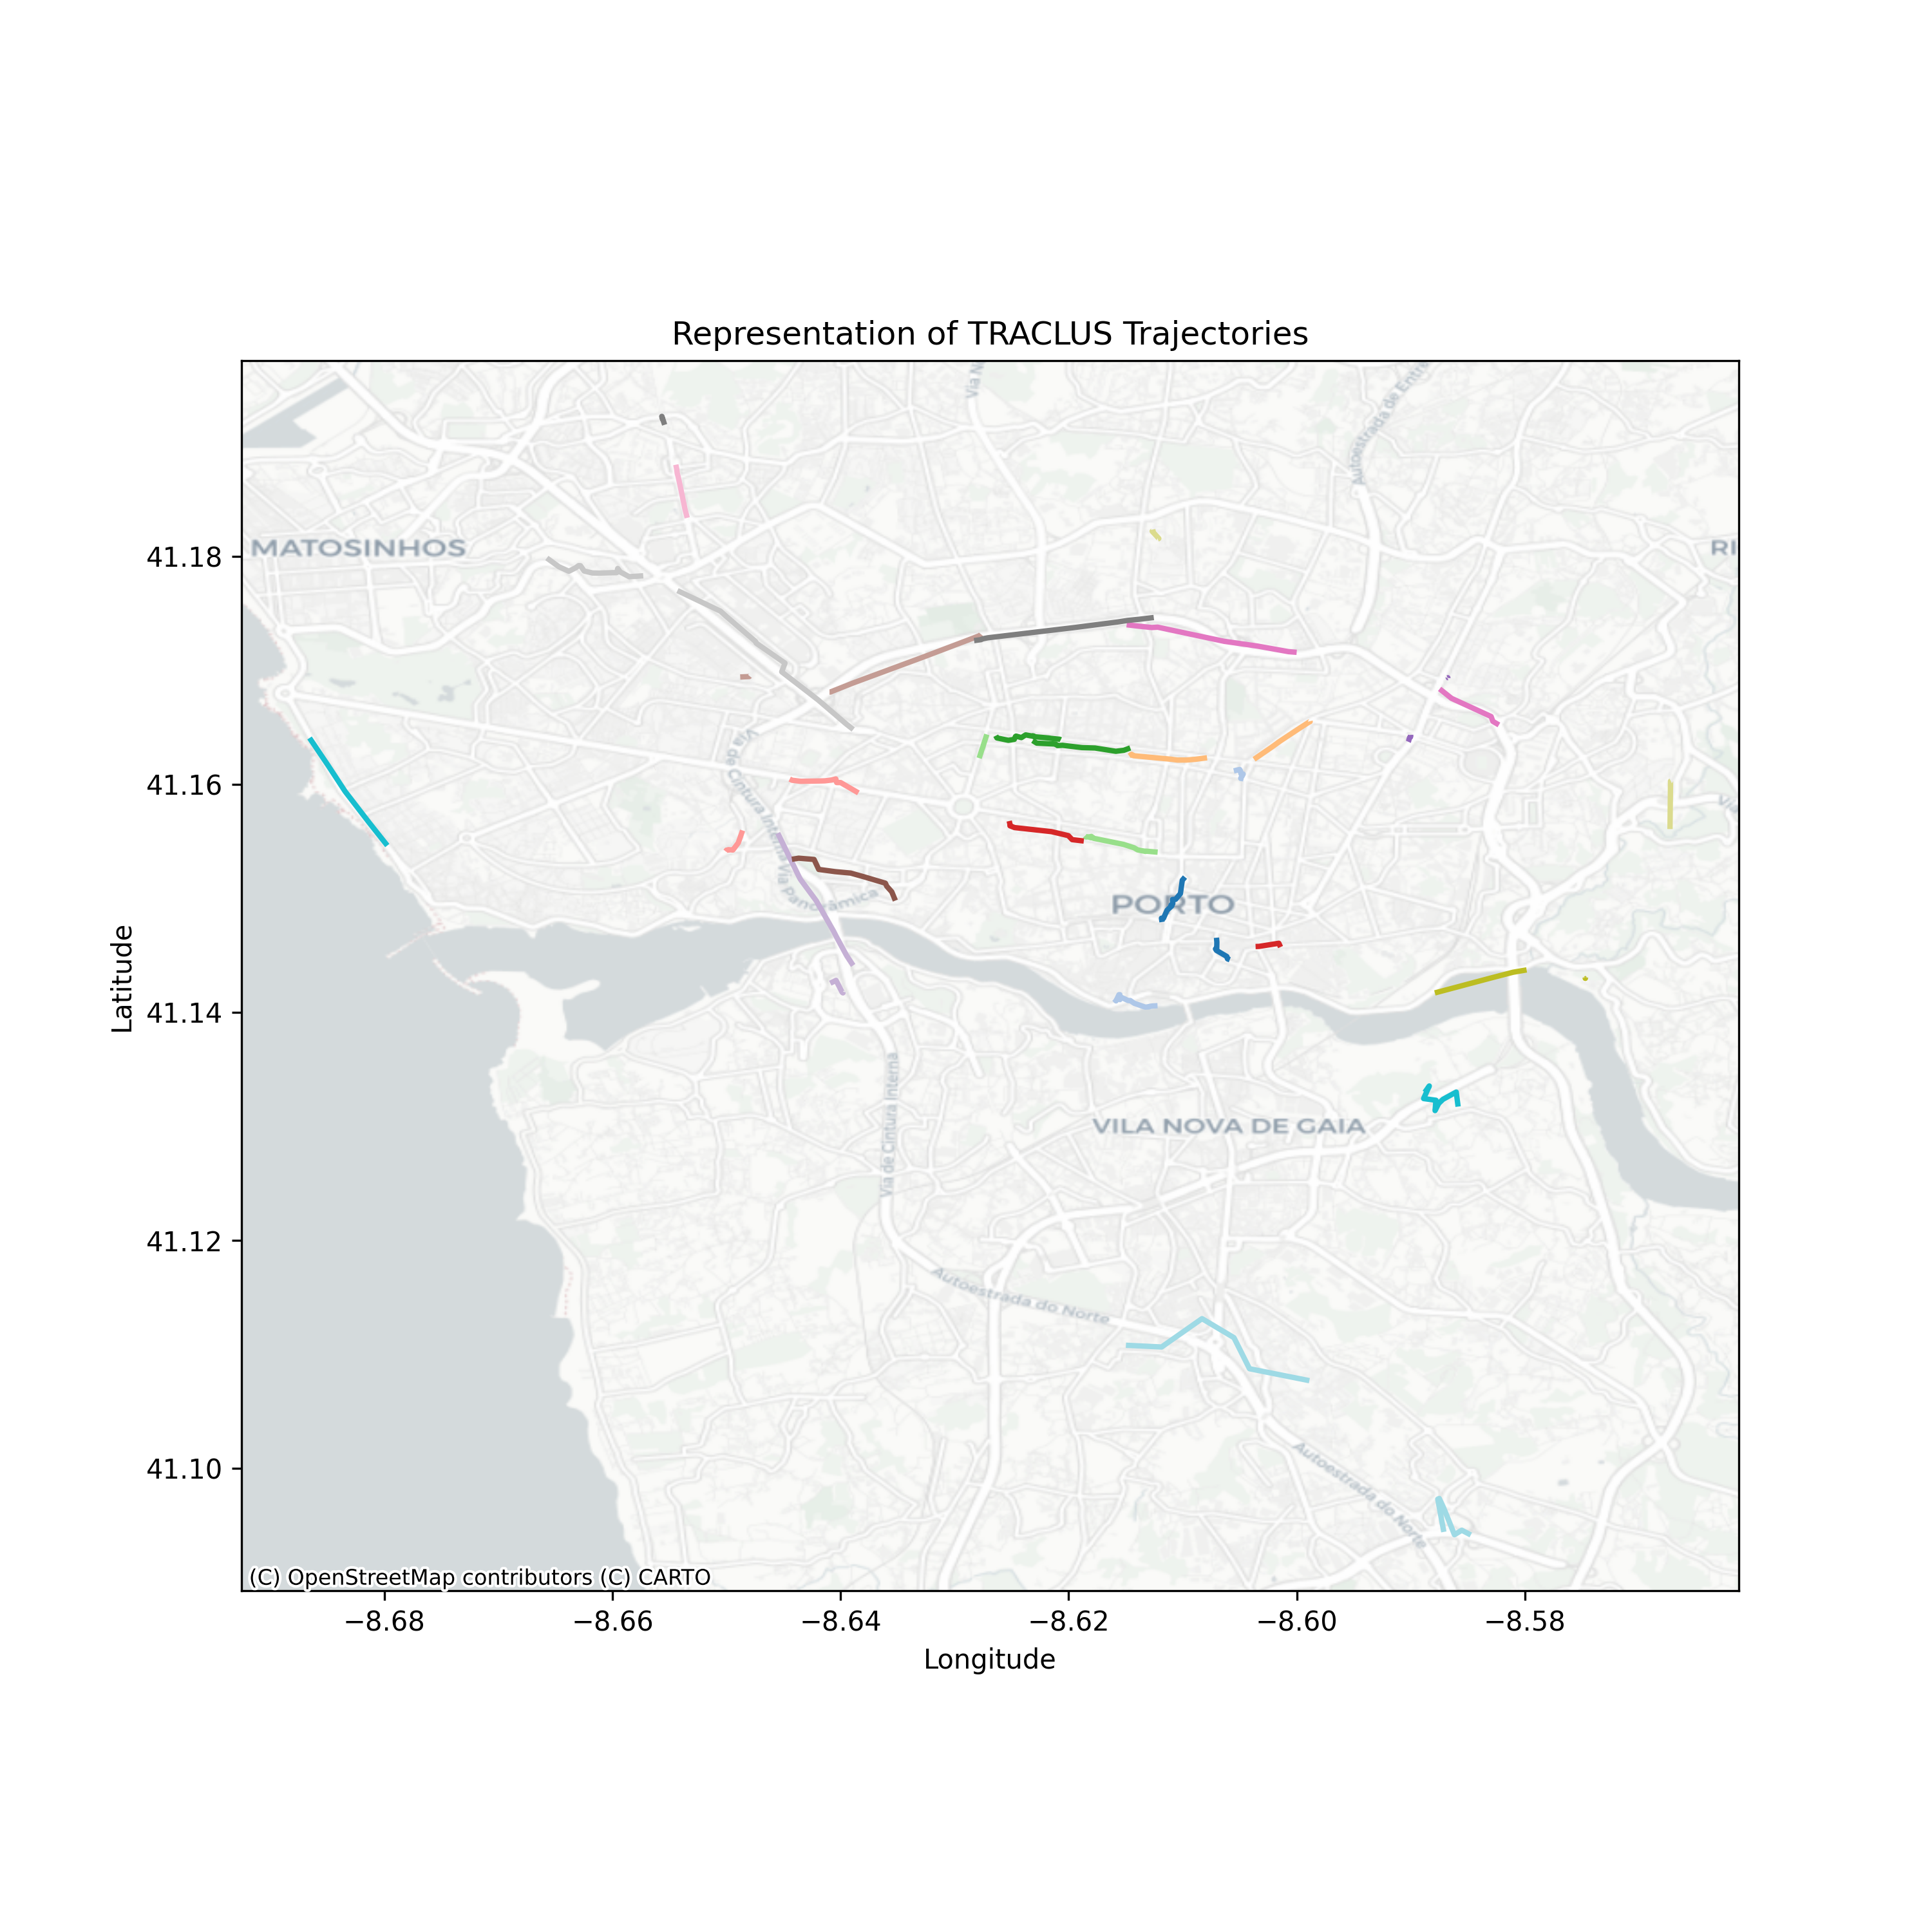
\includegraphics[width=0.5\textwidth]{img/Taxis/map_optics_auto.png}
    \caption{Resultados con todos los algoritmos en OPTICS.}
    \label{fig:taxis_algorith_optics}
\end{figure}

\FloatBarrier

De la misma forma DBSCAN y HDBSCAN, ambas tienen los mismos resultados en cada algoritmo, aun cambiando el resto de datos, los diferentes algoritmos no parecían variar el resultado.

\begin{figure}[h!]
    \centering
    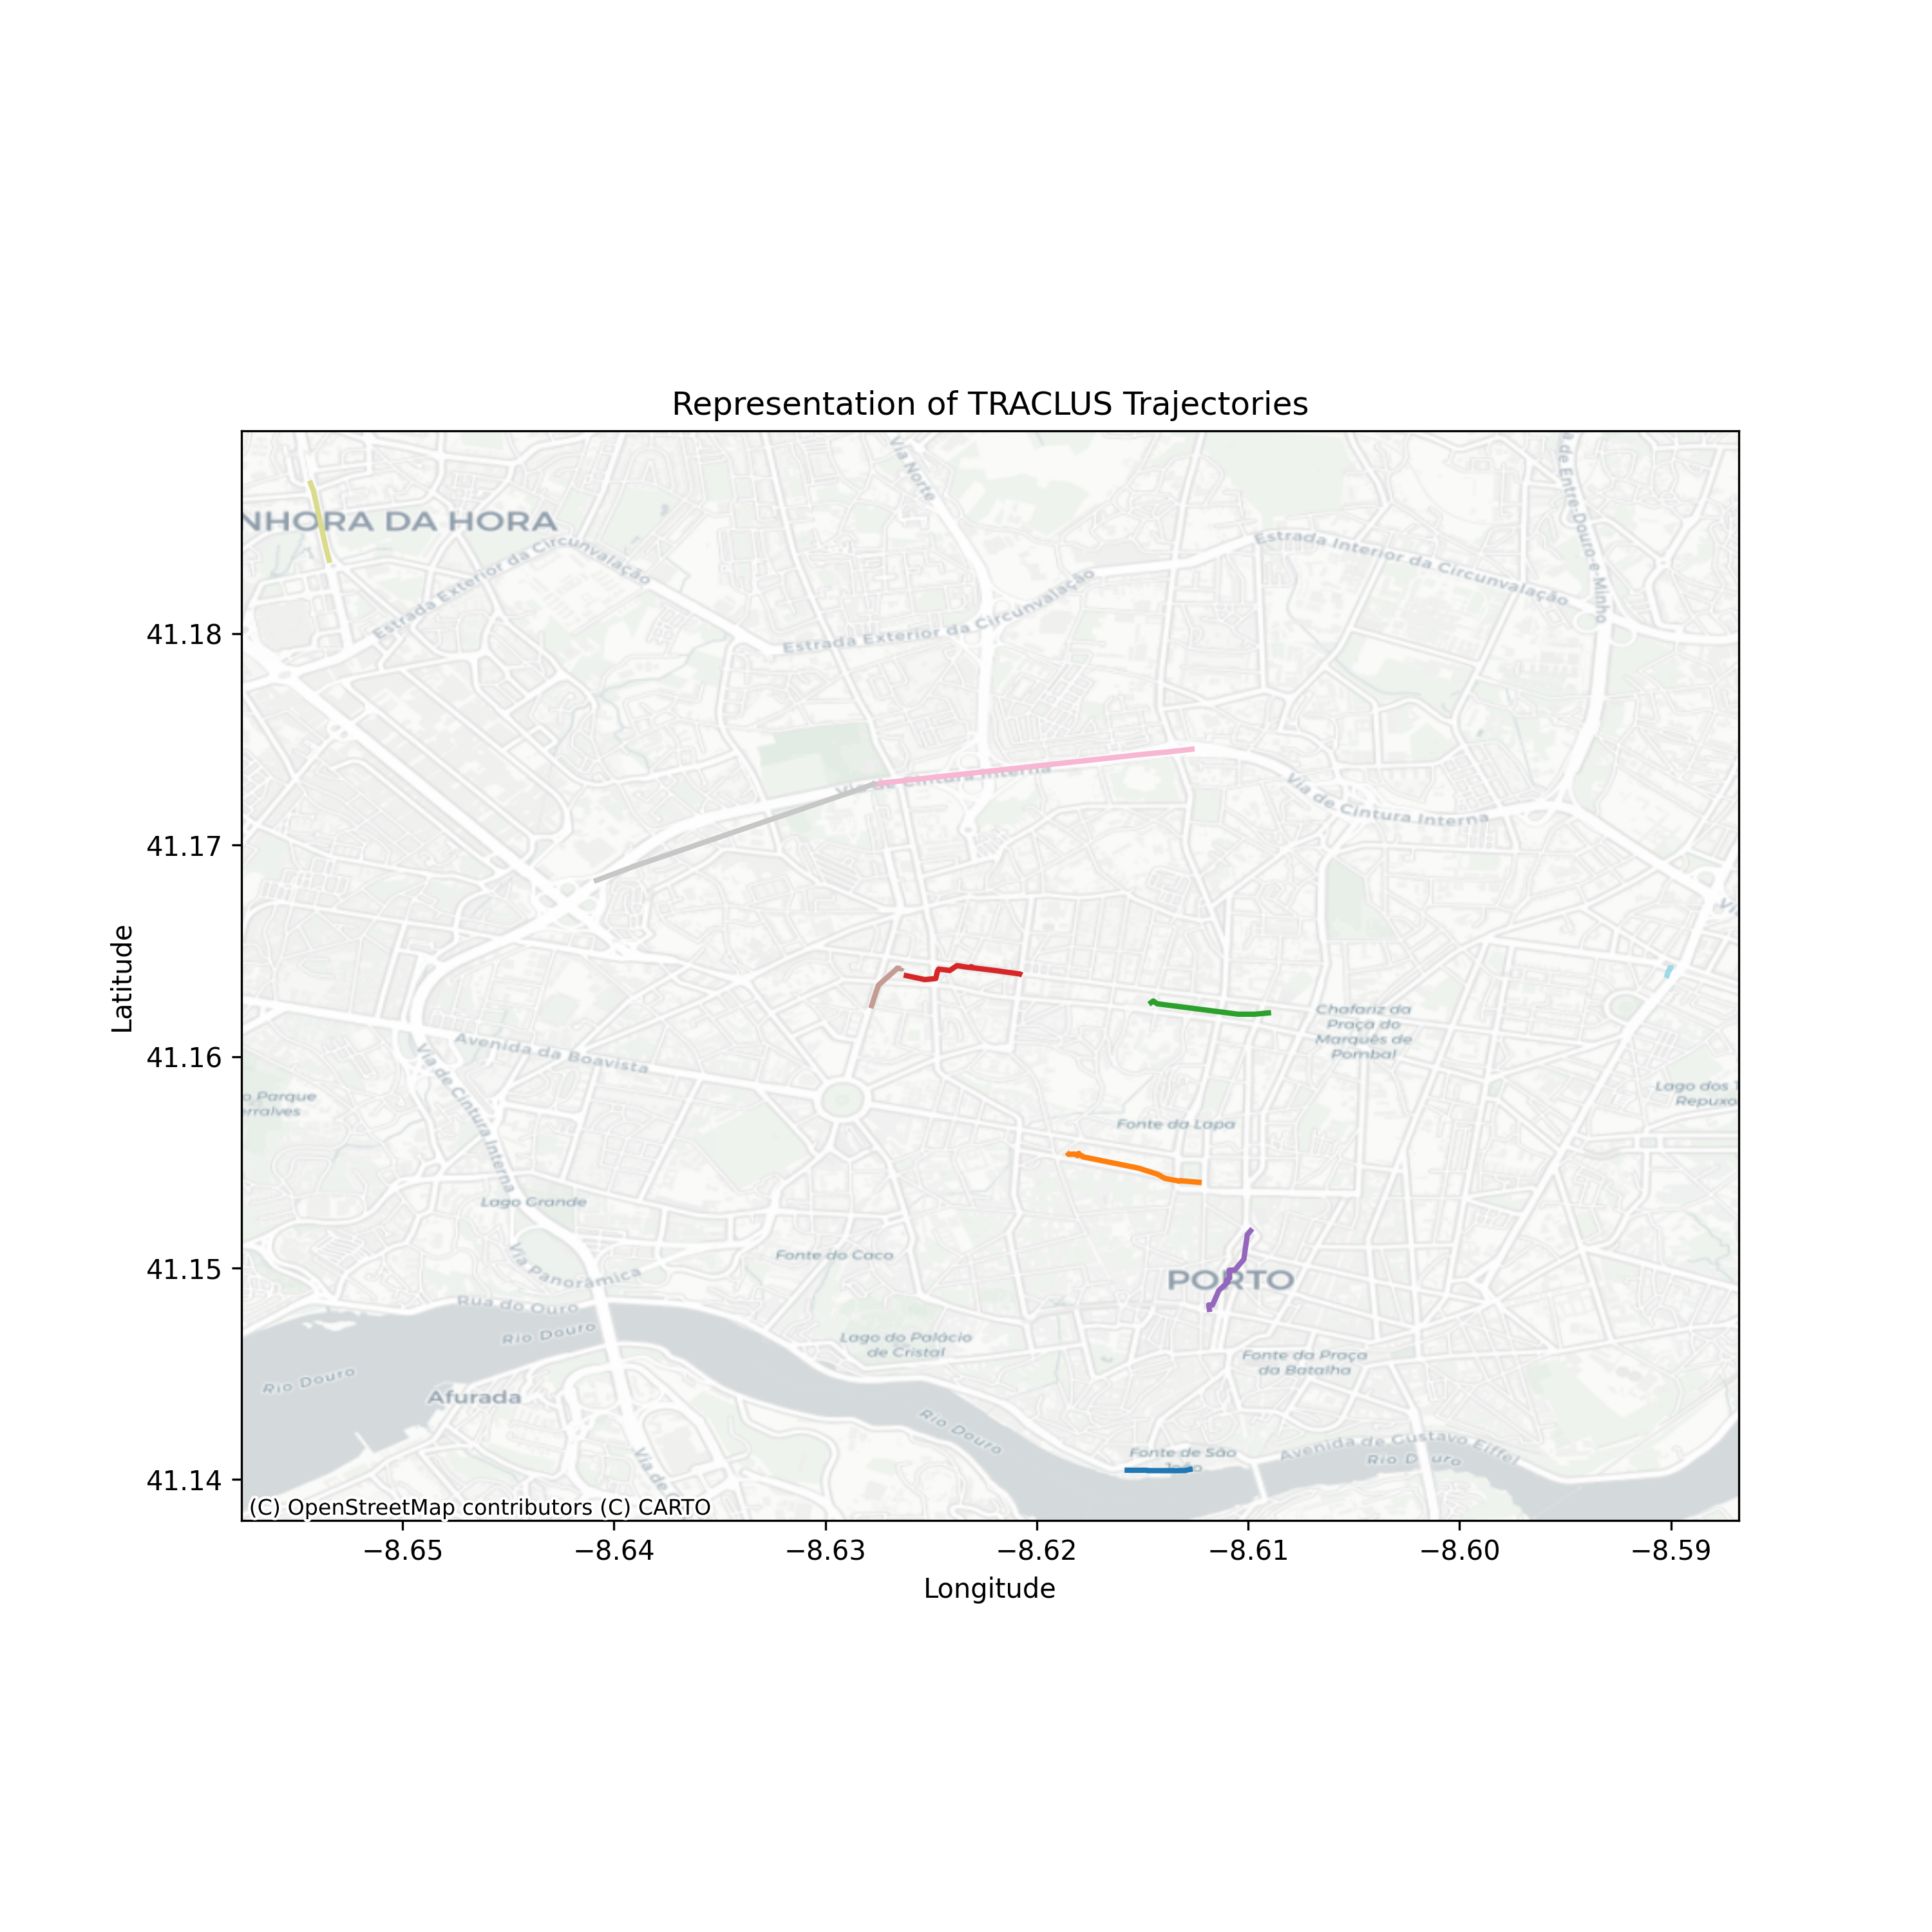
\includegraphics[width=0.5\textwidth]{img/Taxis/map_dbscan_auto.png}
    \caption{Resultados con todos los algoritmos en DBSCAN.}
    \label{fig:taxis_algorith_dbscan}
\end{figure}

\FloatBarrier

\begin{figure}[h!]
    \centering
    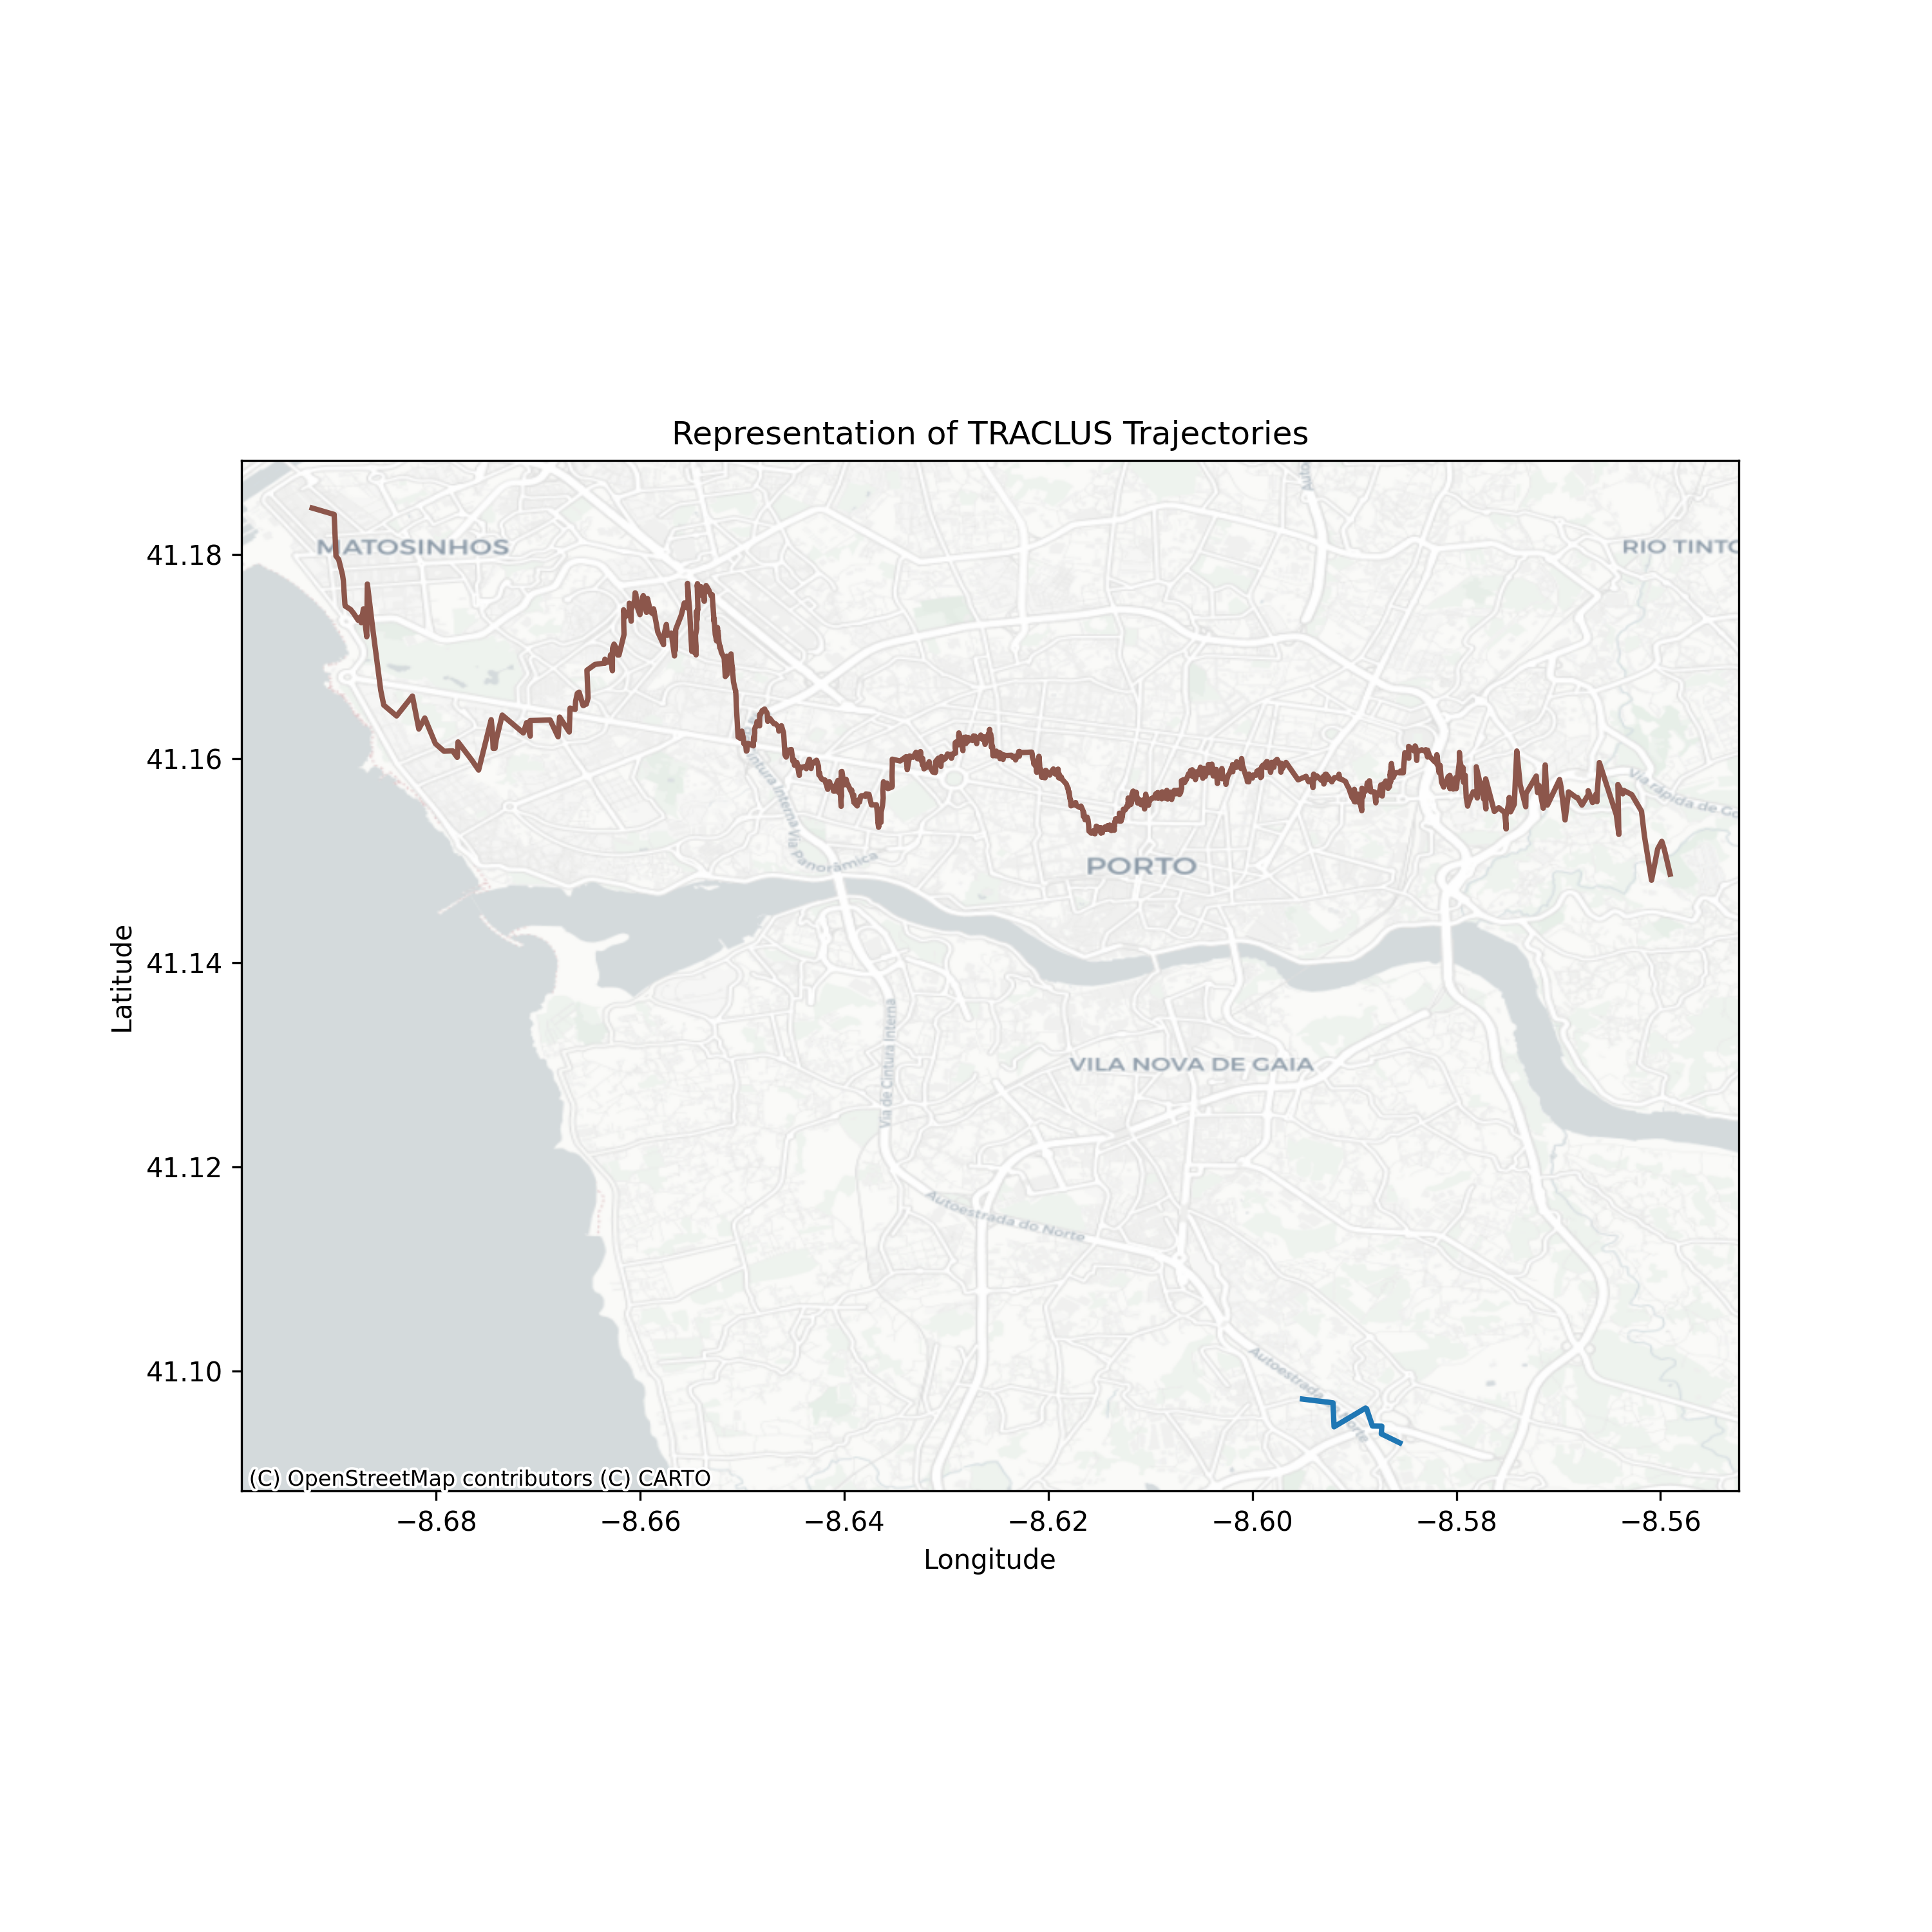
\includegraphics[width=0.5\textwidth]{img/Taxis/map_hdbscan_auto.png}
    \caption{Resultados con todos los algoritmos en HDBSCAN.}
    \label{fig:taxis_algorith_hdbscan}
\end{figure}

\FloatBarrier

De la misma forma que los resultados eran afectados por los algoritmos en este conjunto lo fueran en los demás.

- \textbf{Conjunto Movebank}: 


\begin{figure}[h!]
    \centering
    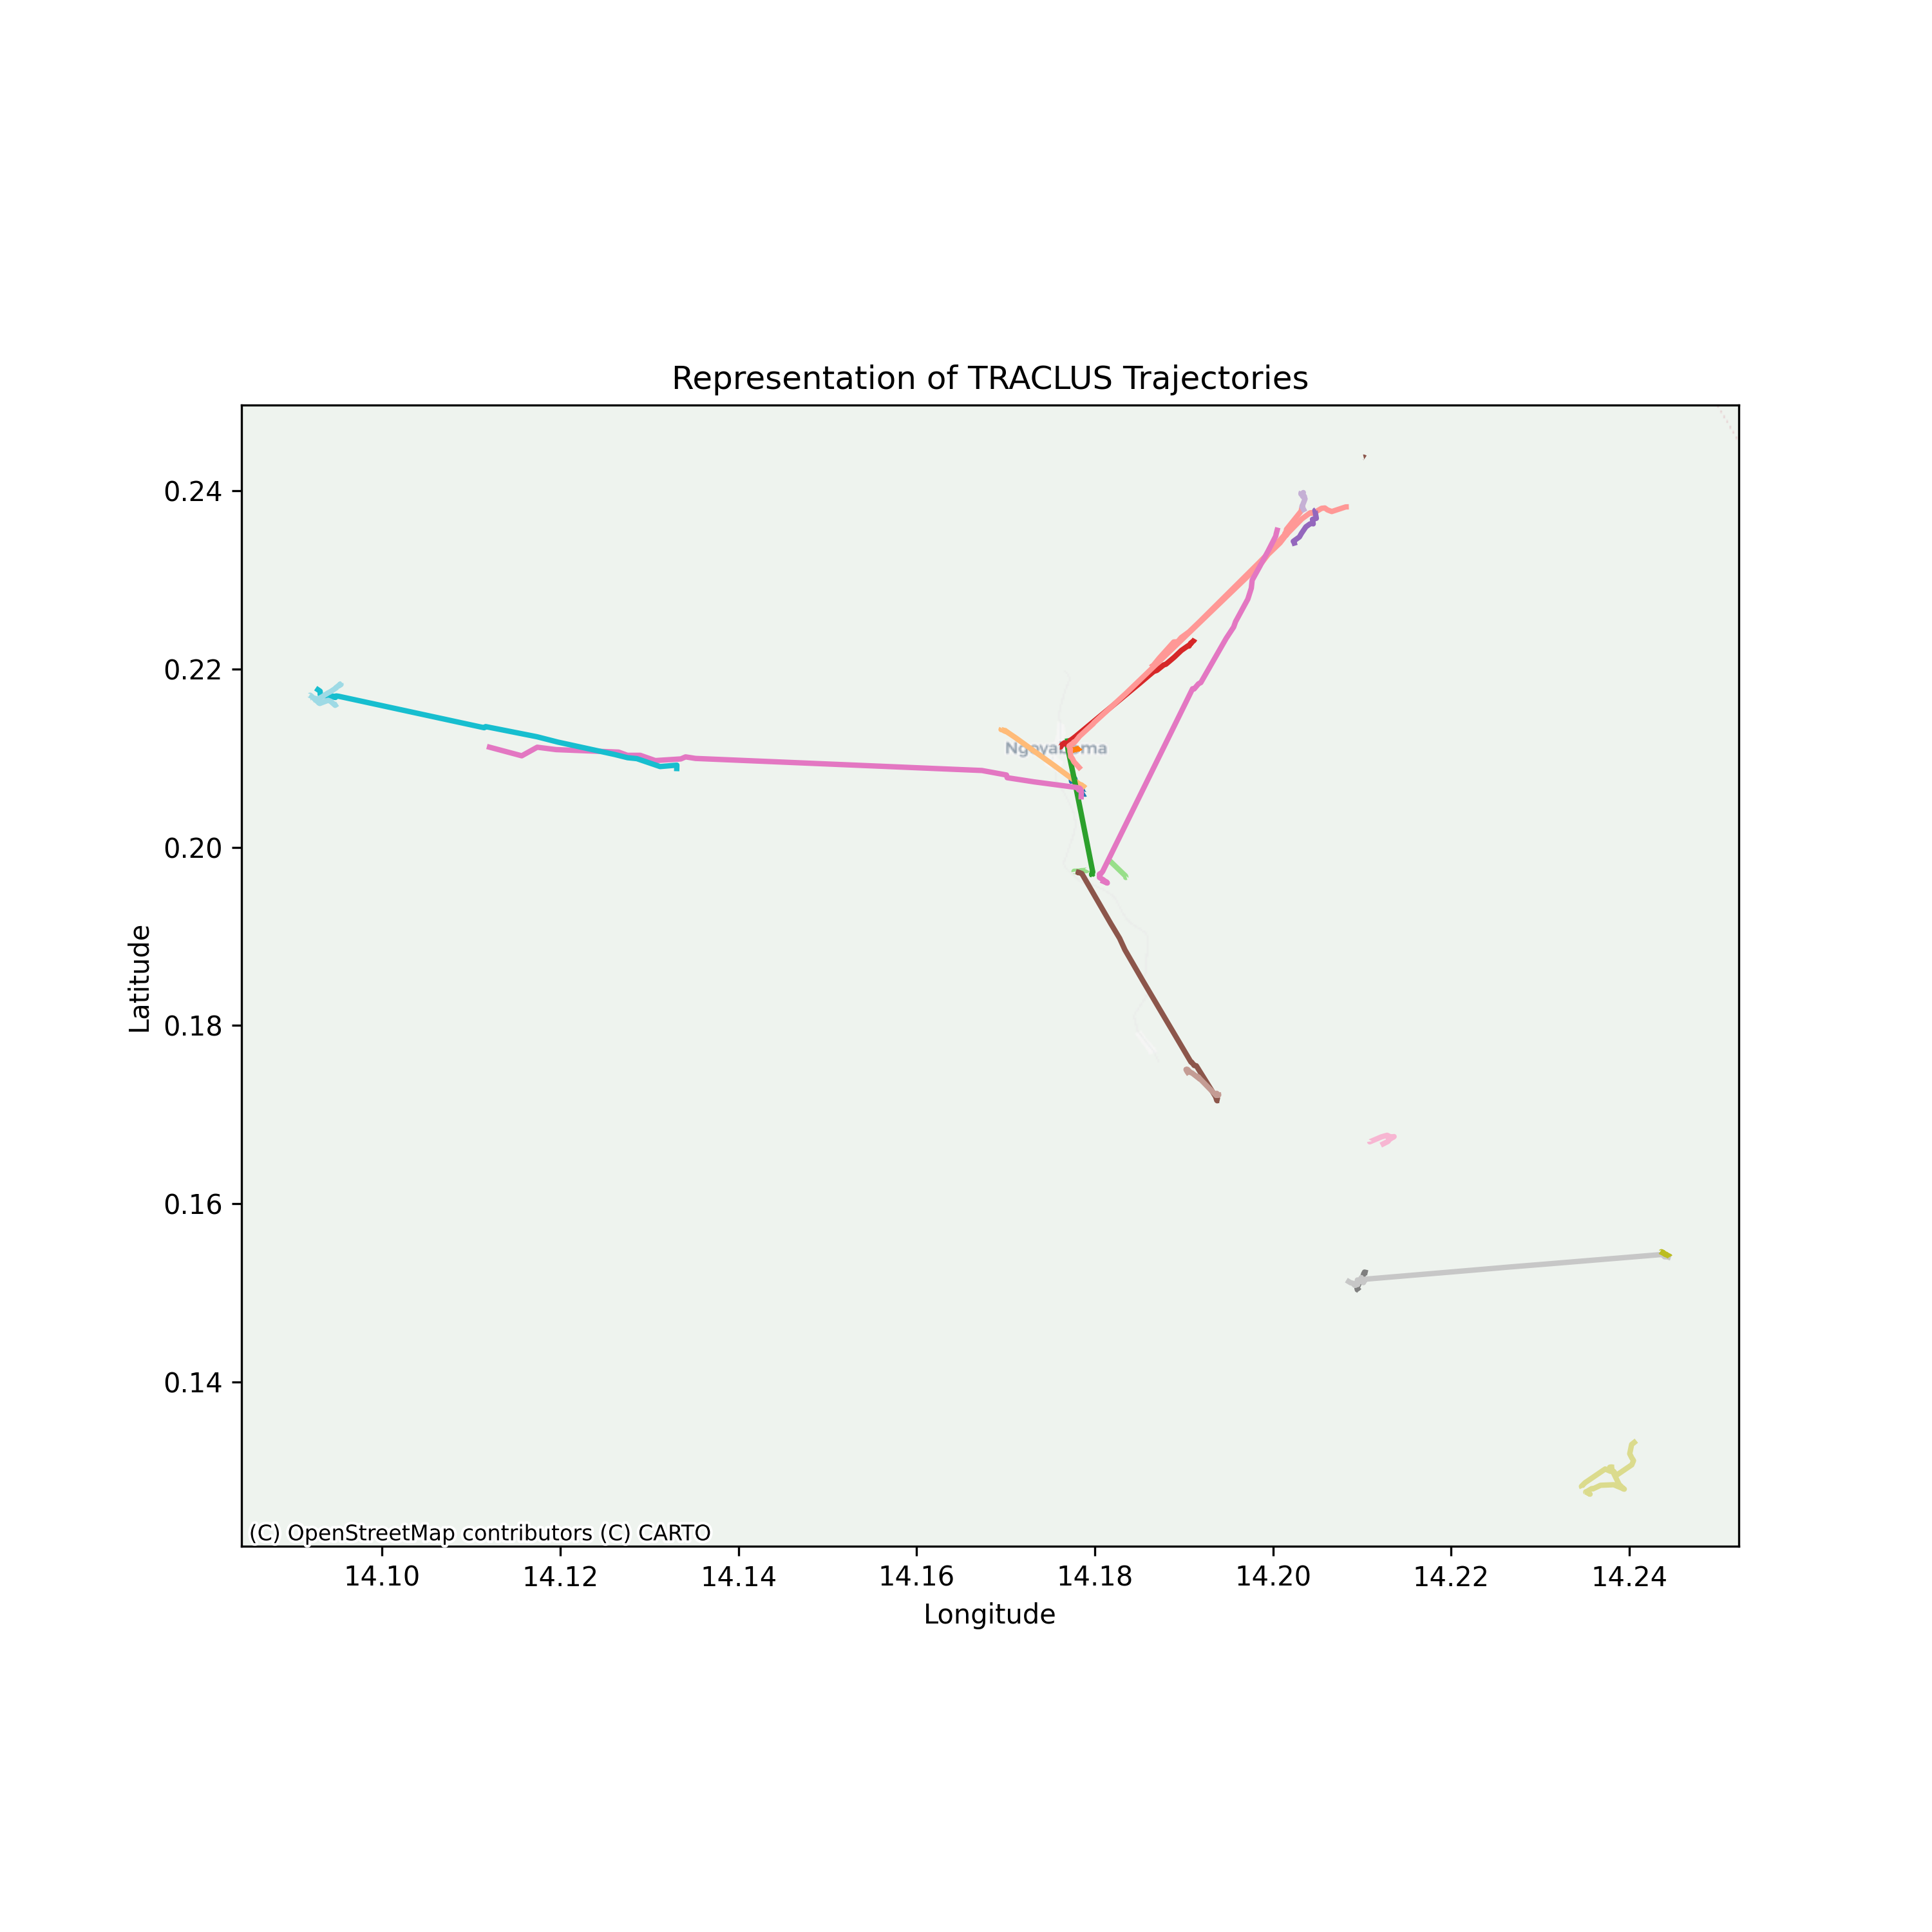
\includegraphics[width=0.5\textwidth]{img/Movebank/map_optics_auto.png}
    \caption{Resultados con todos los algoritmos en OPTICS y HDBSCAN.}
    \label{fig:movebank_algorith_optics}
\end{figure}

\FloatBarrier

\begin{figure}[h!]
    \centering
    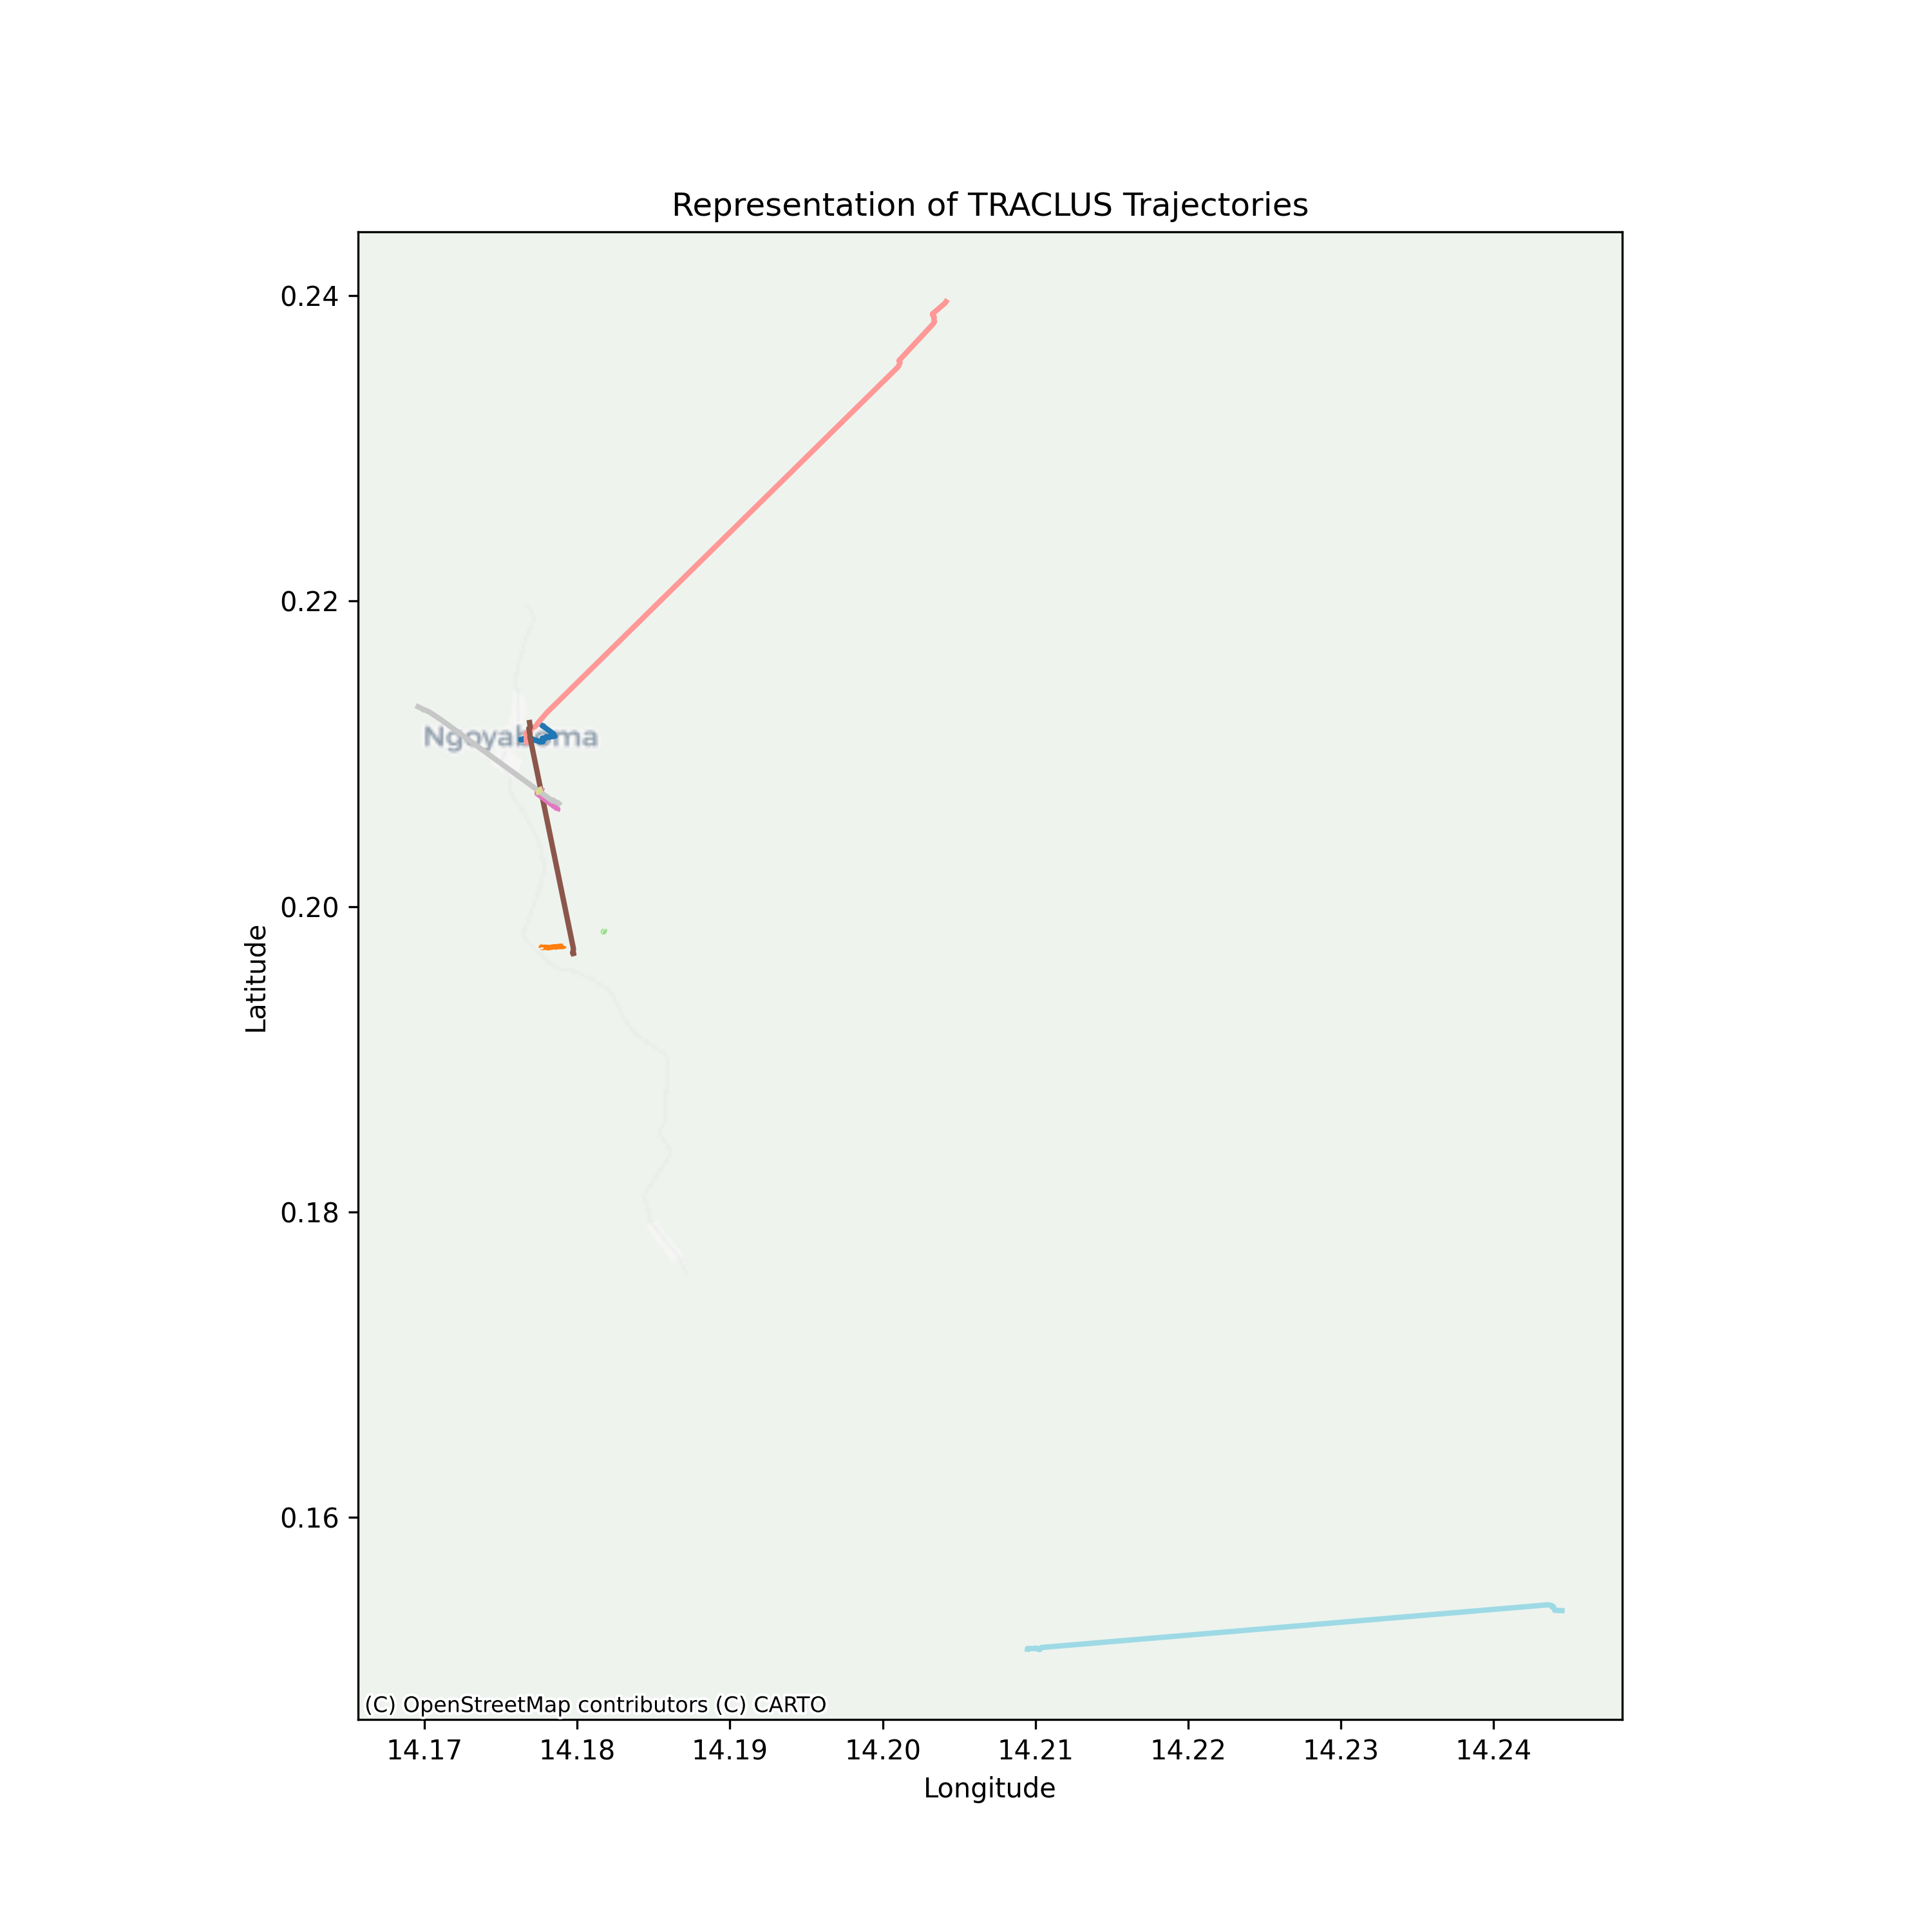
\includegraphics[width=0.5\textwidth]{img/Movebank/map_dbscan_auto.png}
    \caption{Resultados con todos los algoritmos en DBSCAN.}
    \label{fig:movebank_algorith_dbscan}
\end{figure}

\FloatBarrier

\begin{figure}[h!]
    \centering
    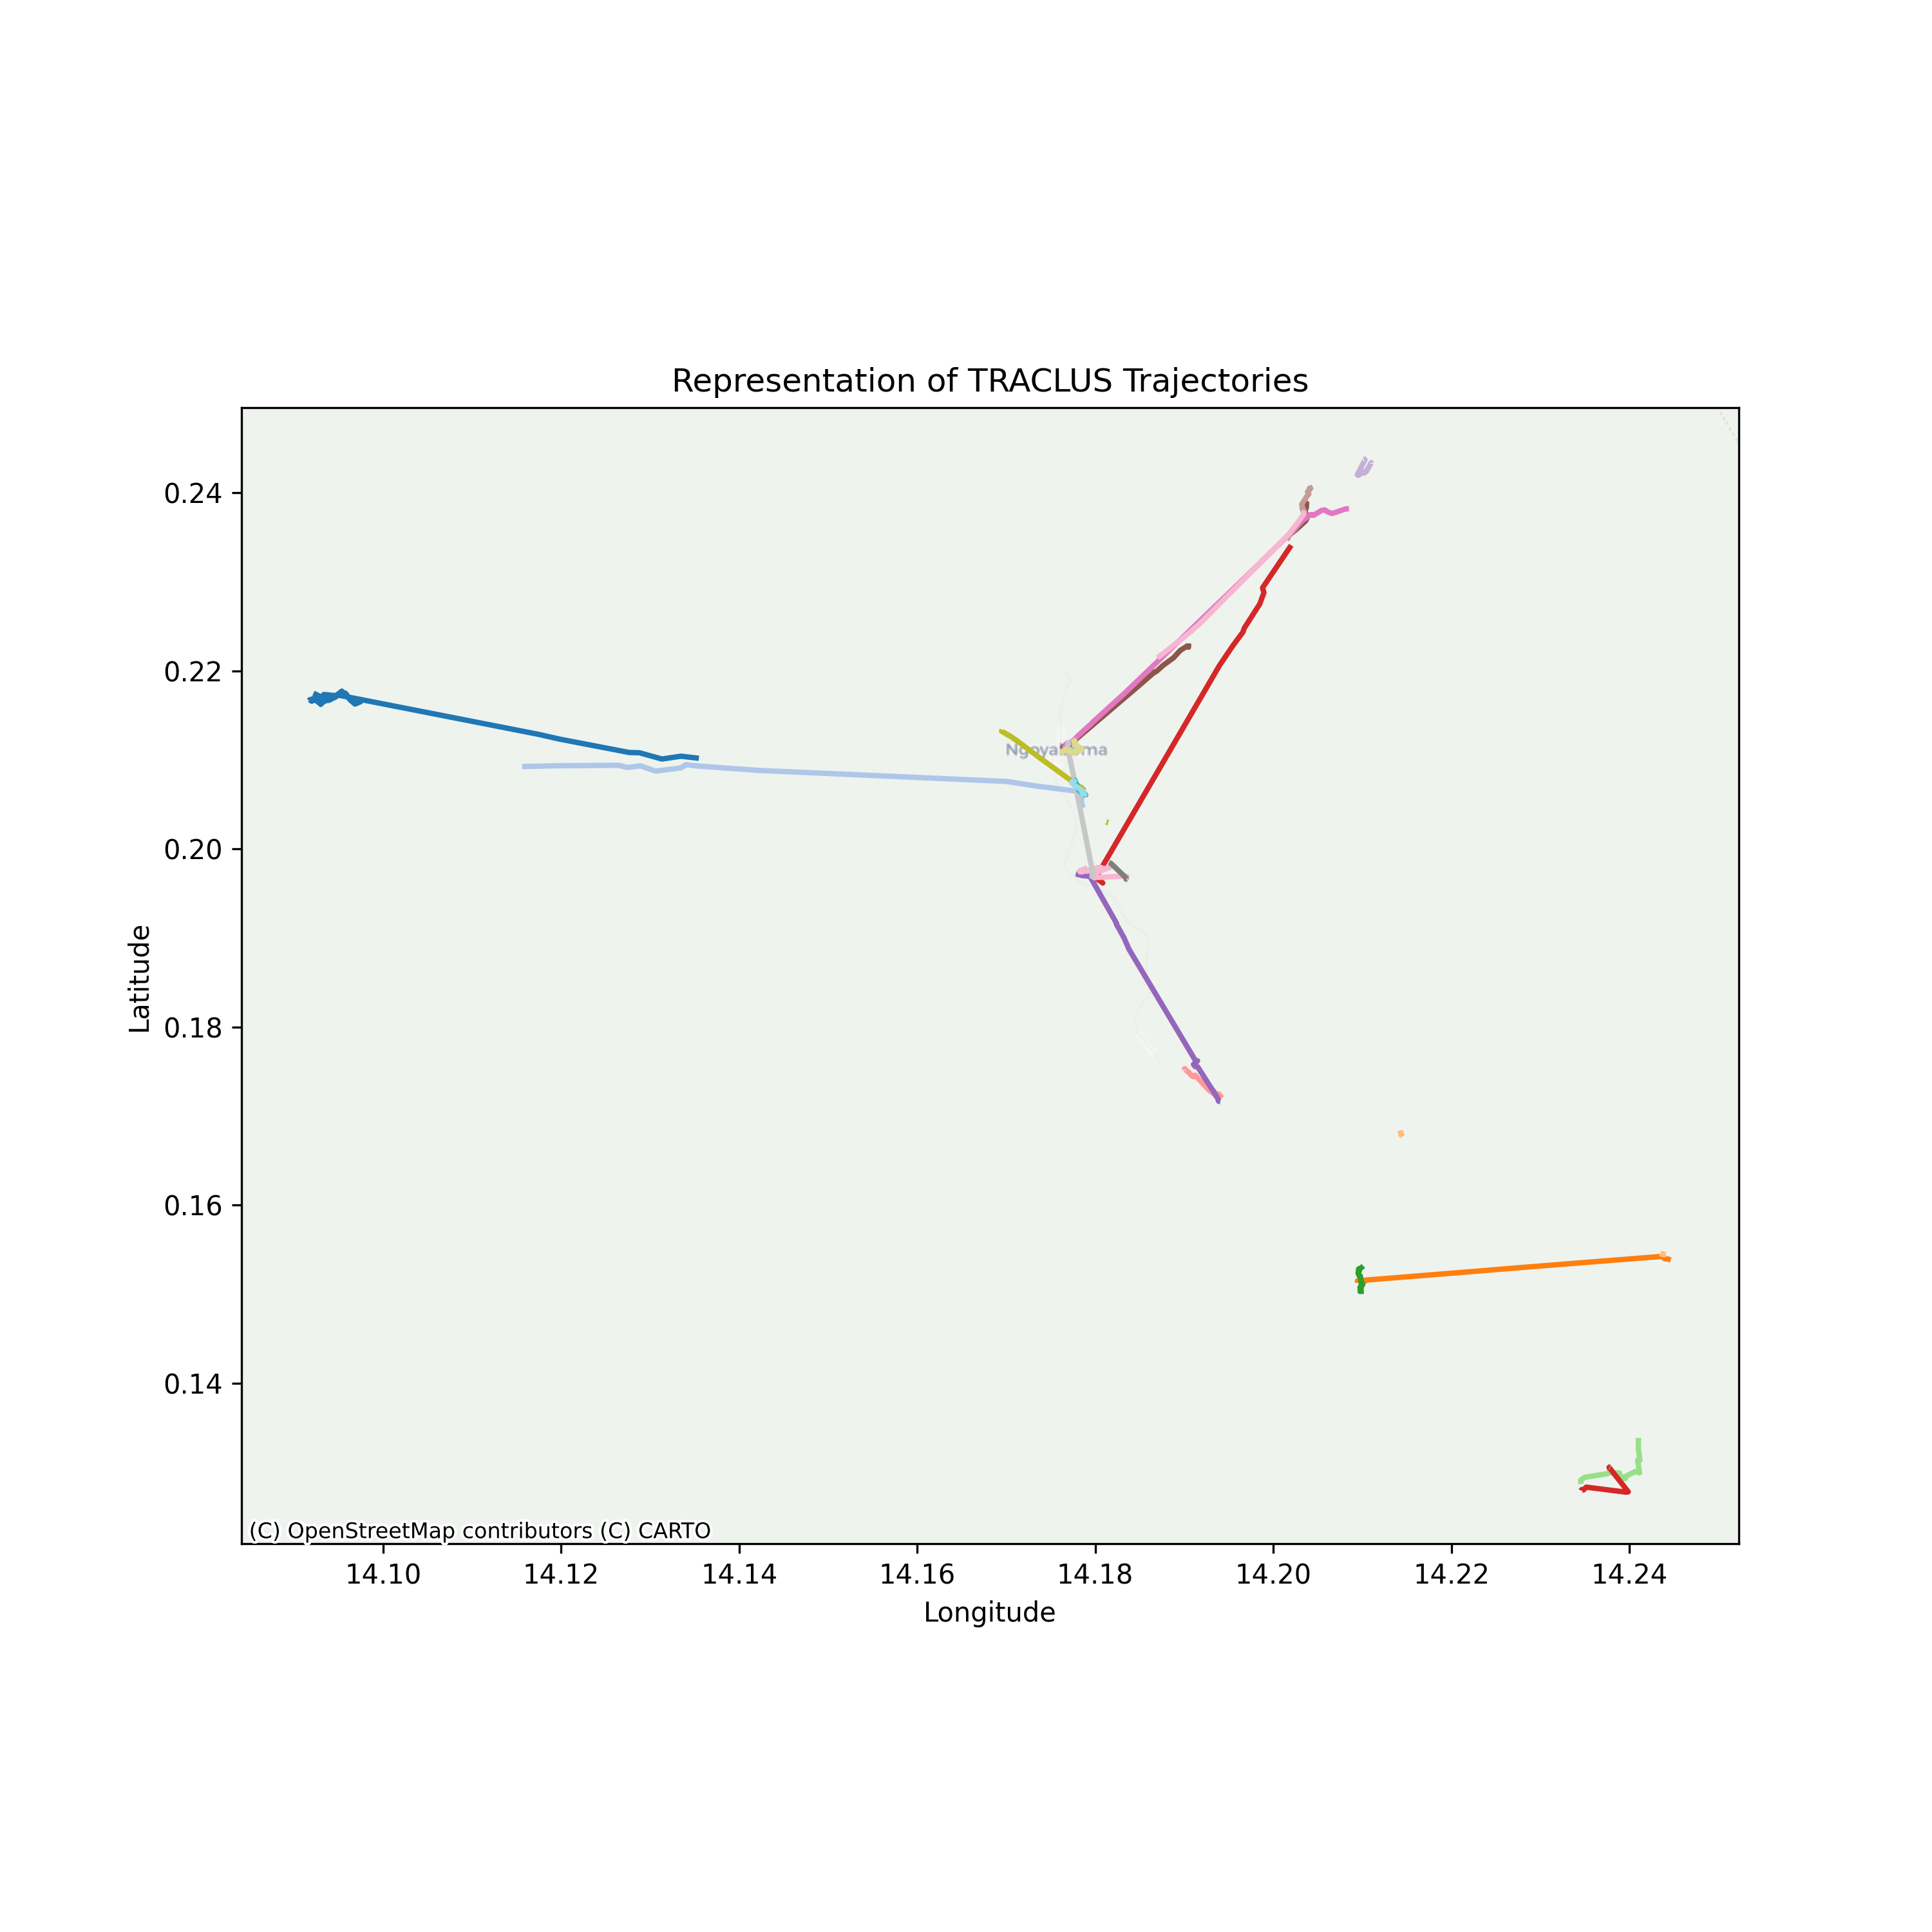
\includegraphics[width=0.5\textwidth]{img/Movebank/map_hdbscan_auto.png}
    \caption{Resultados con todos los algoritmos en HDBSCAN.}
    \label{fig:movebank_algorith_hdbscan}
\end{figure}

\FloatBarrier

- \textbf{Conjunto Geolife}: 


\begin{figure}[h!]
    \centering
    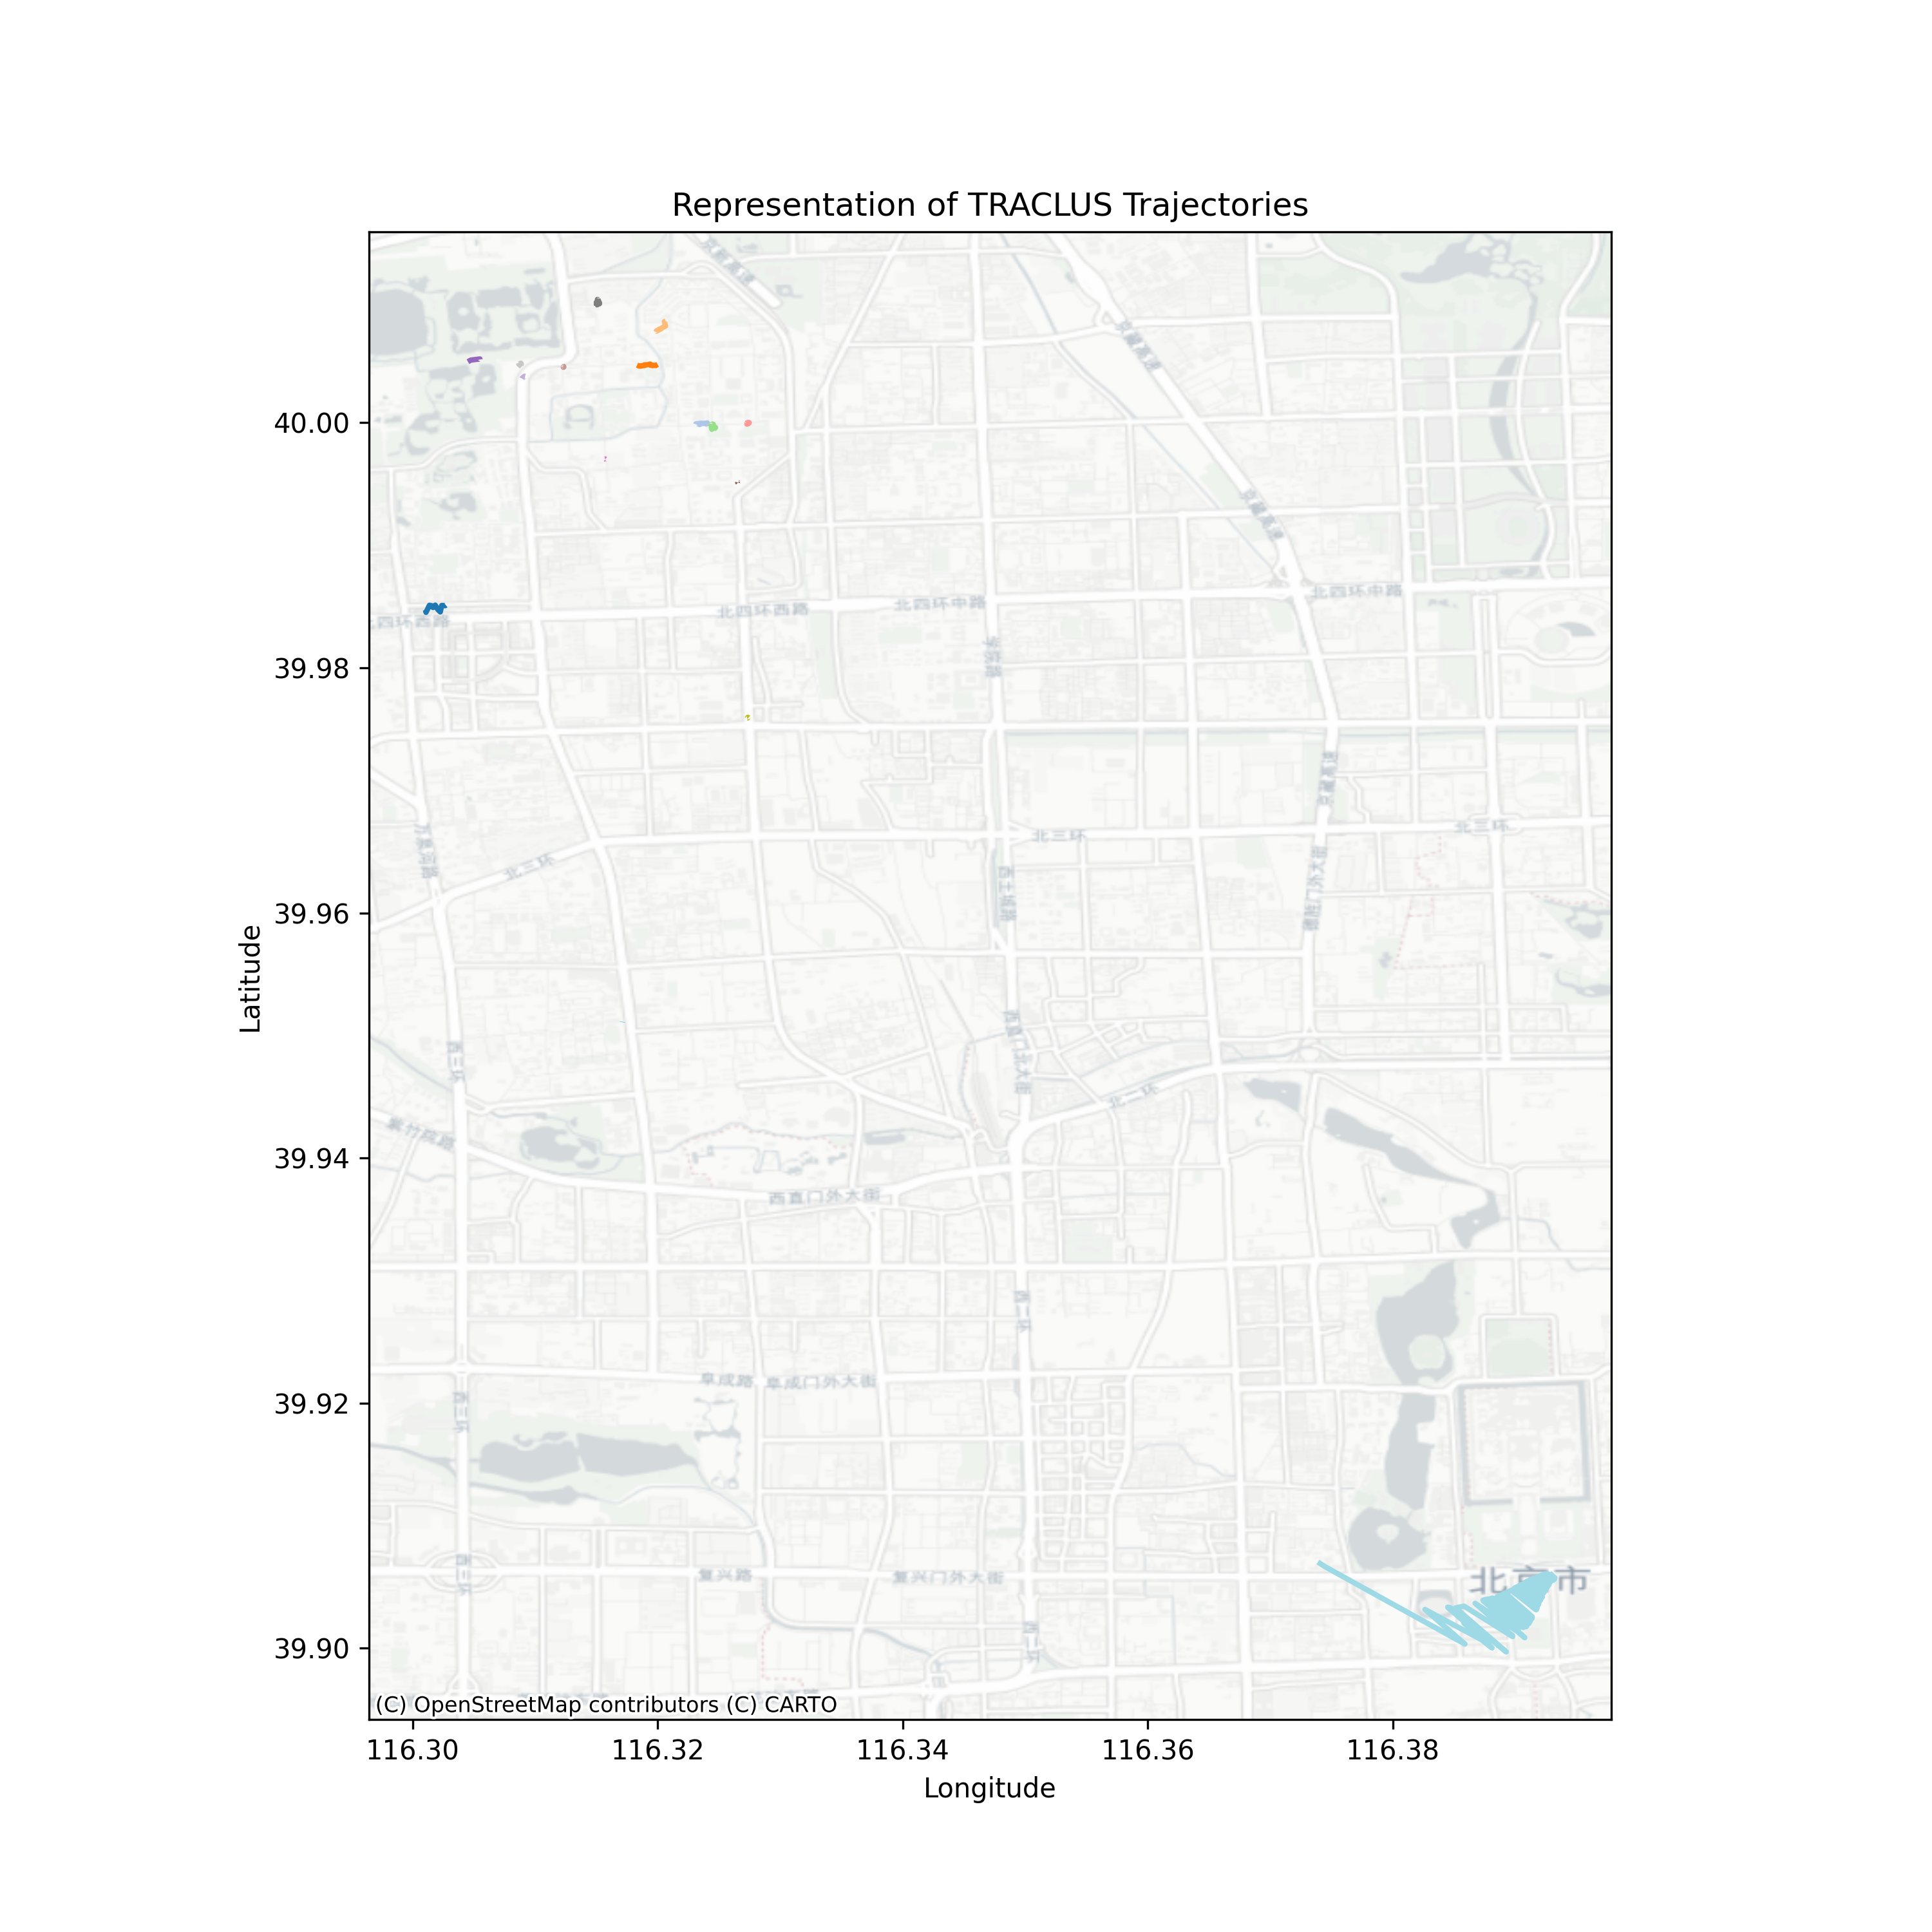
\includegraphics[width=0.5\textwidth]{img/Geolife/map_optics_auto.png}
    \caption{Resultados con todos los algoritmos en OPTICS.}
    \label{fig:geolife_algorith_optics}
\end{figure}

\FloatBarrier

\begin{figure}[h!]
    \centering
    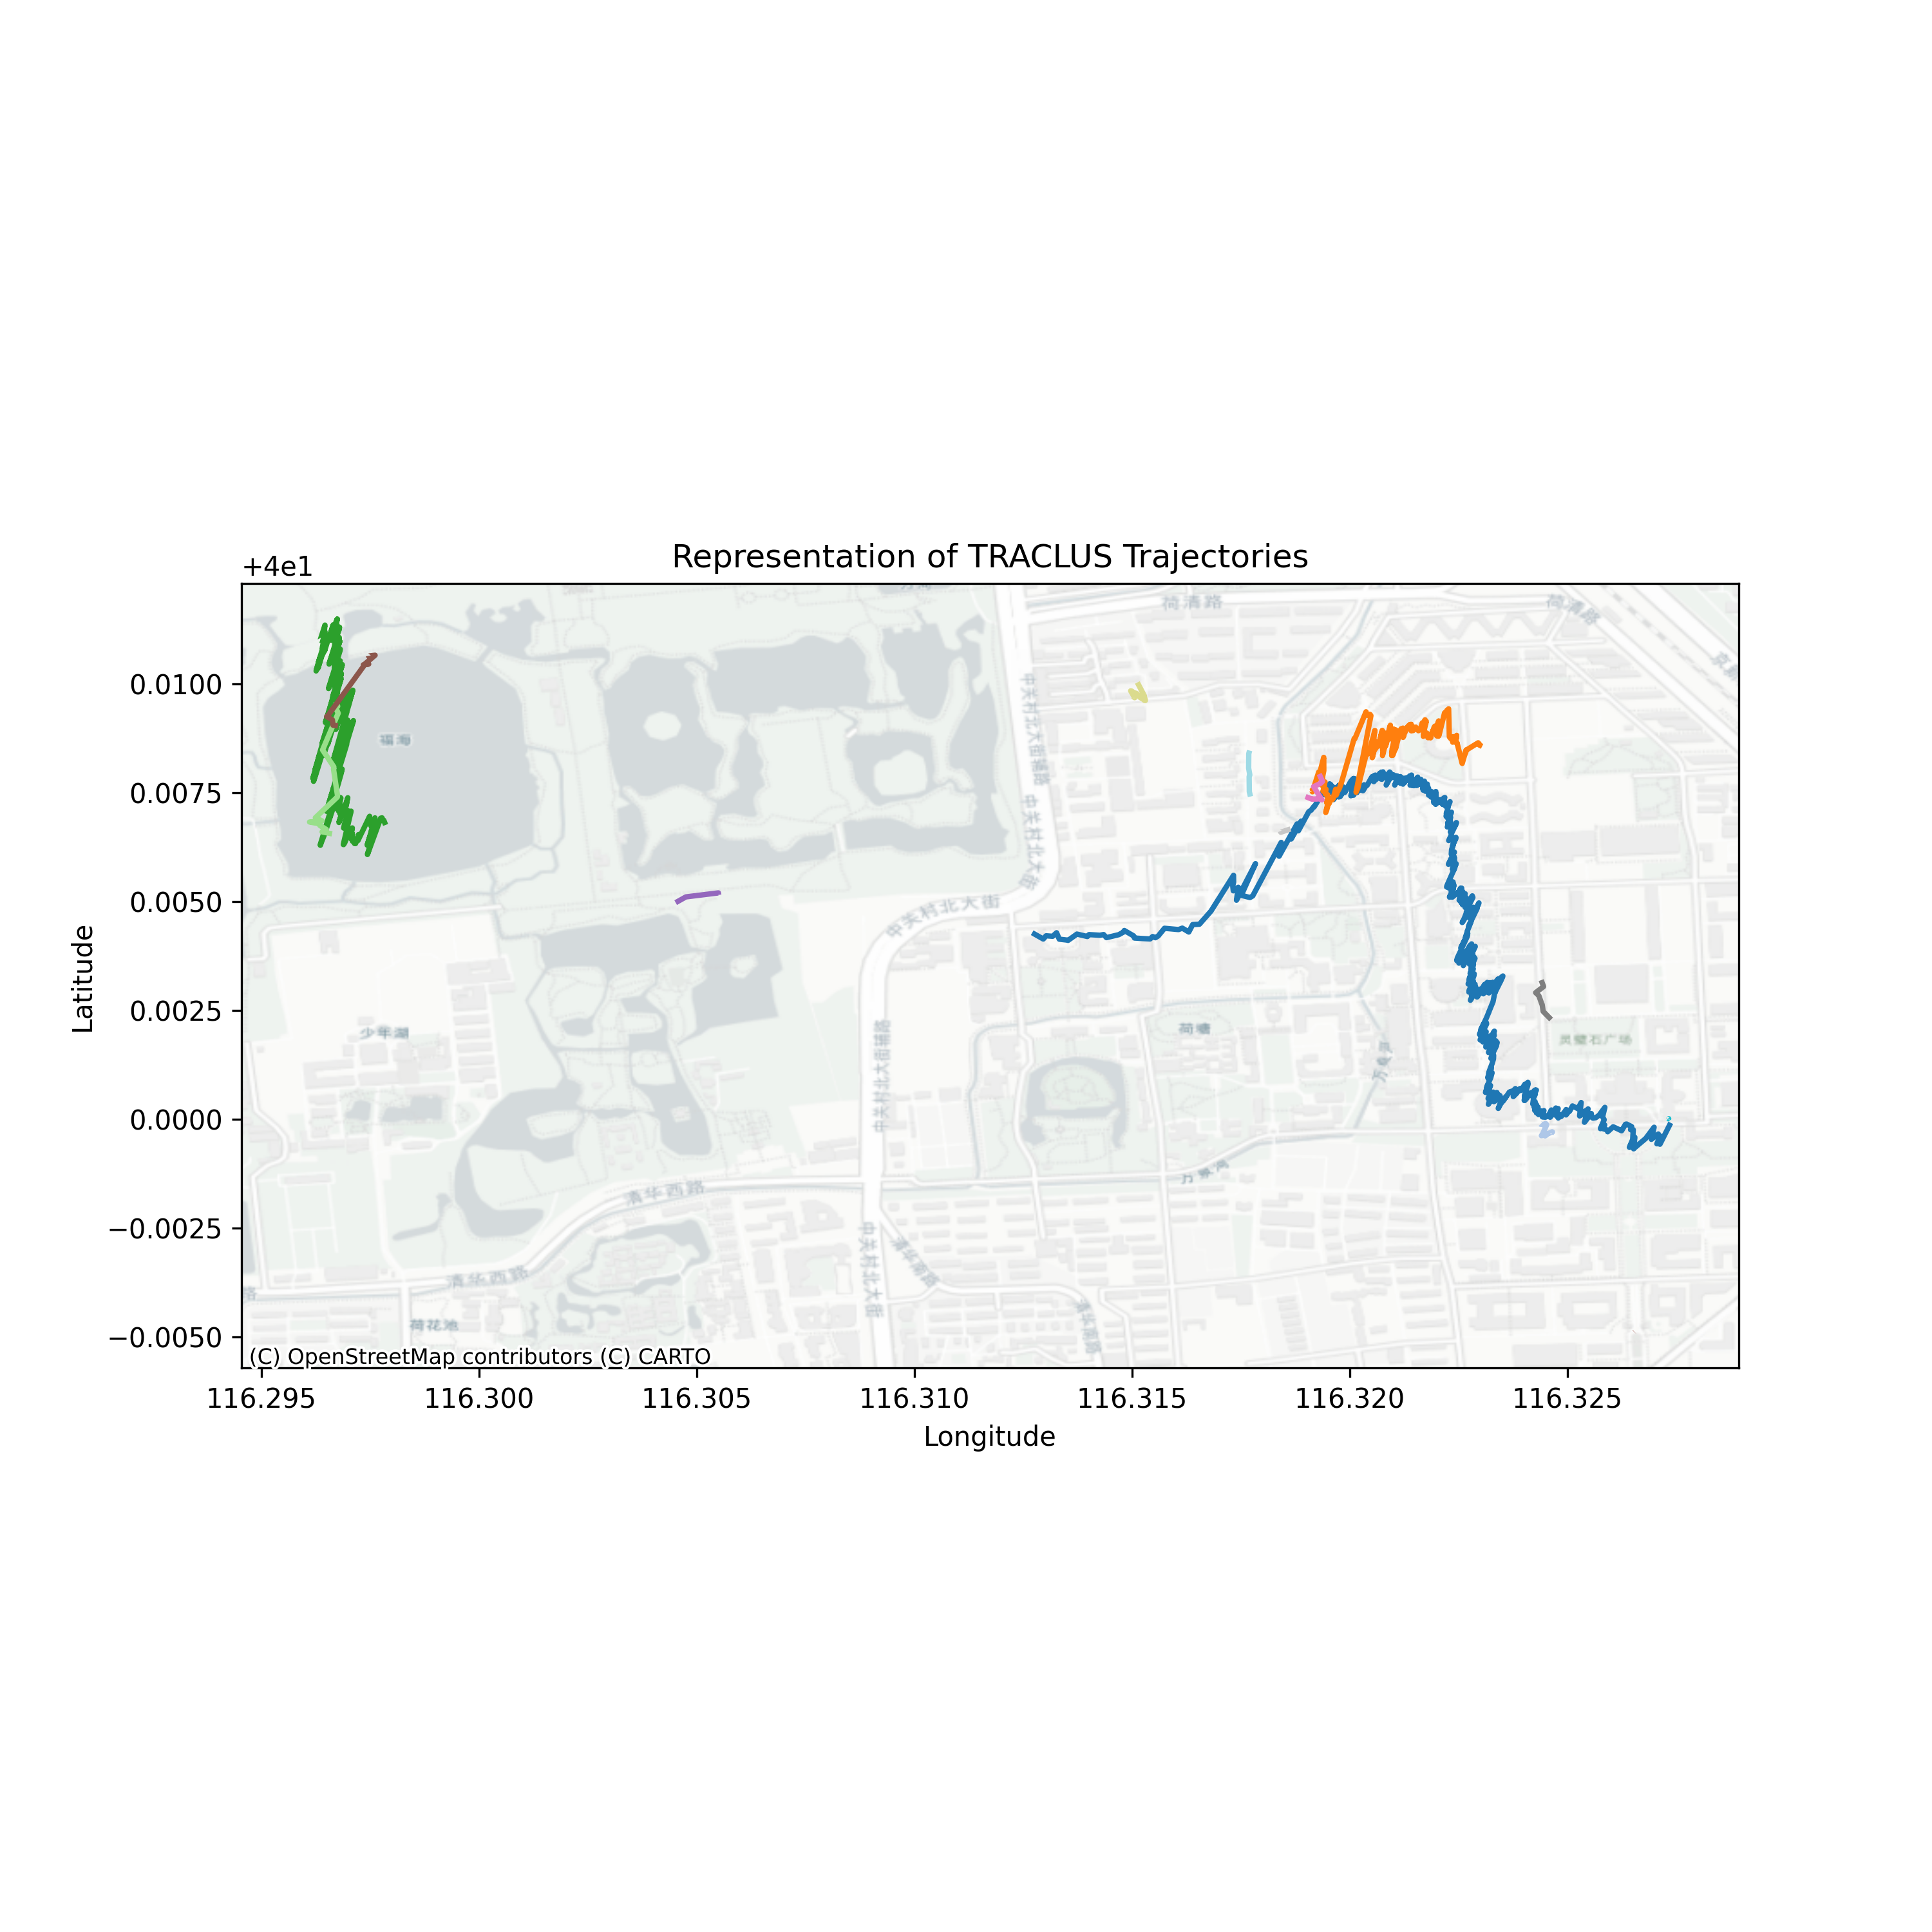
\includegraphics[width=0.5\textwidth]{img/Geolife/map_dbscan_auto.png}
    \caption{Resultados con todos los algoritmos en DBSCAN.}
    \label{fig:geolife_algorith_dbscan}
\end{figure}

\FloatBarrier

\begin{figure}[h!]
    \centering
    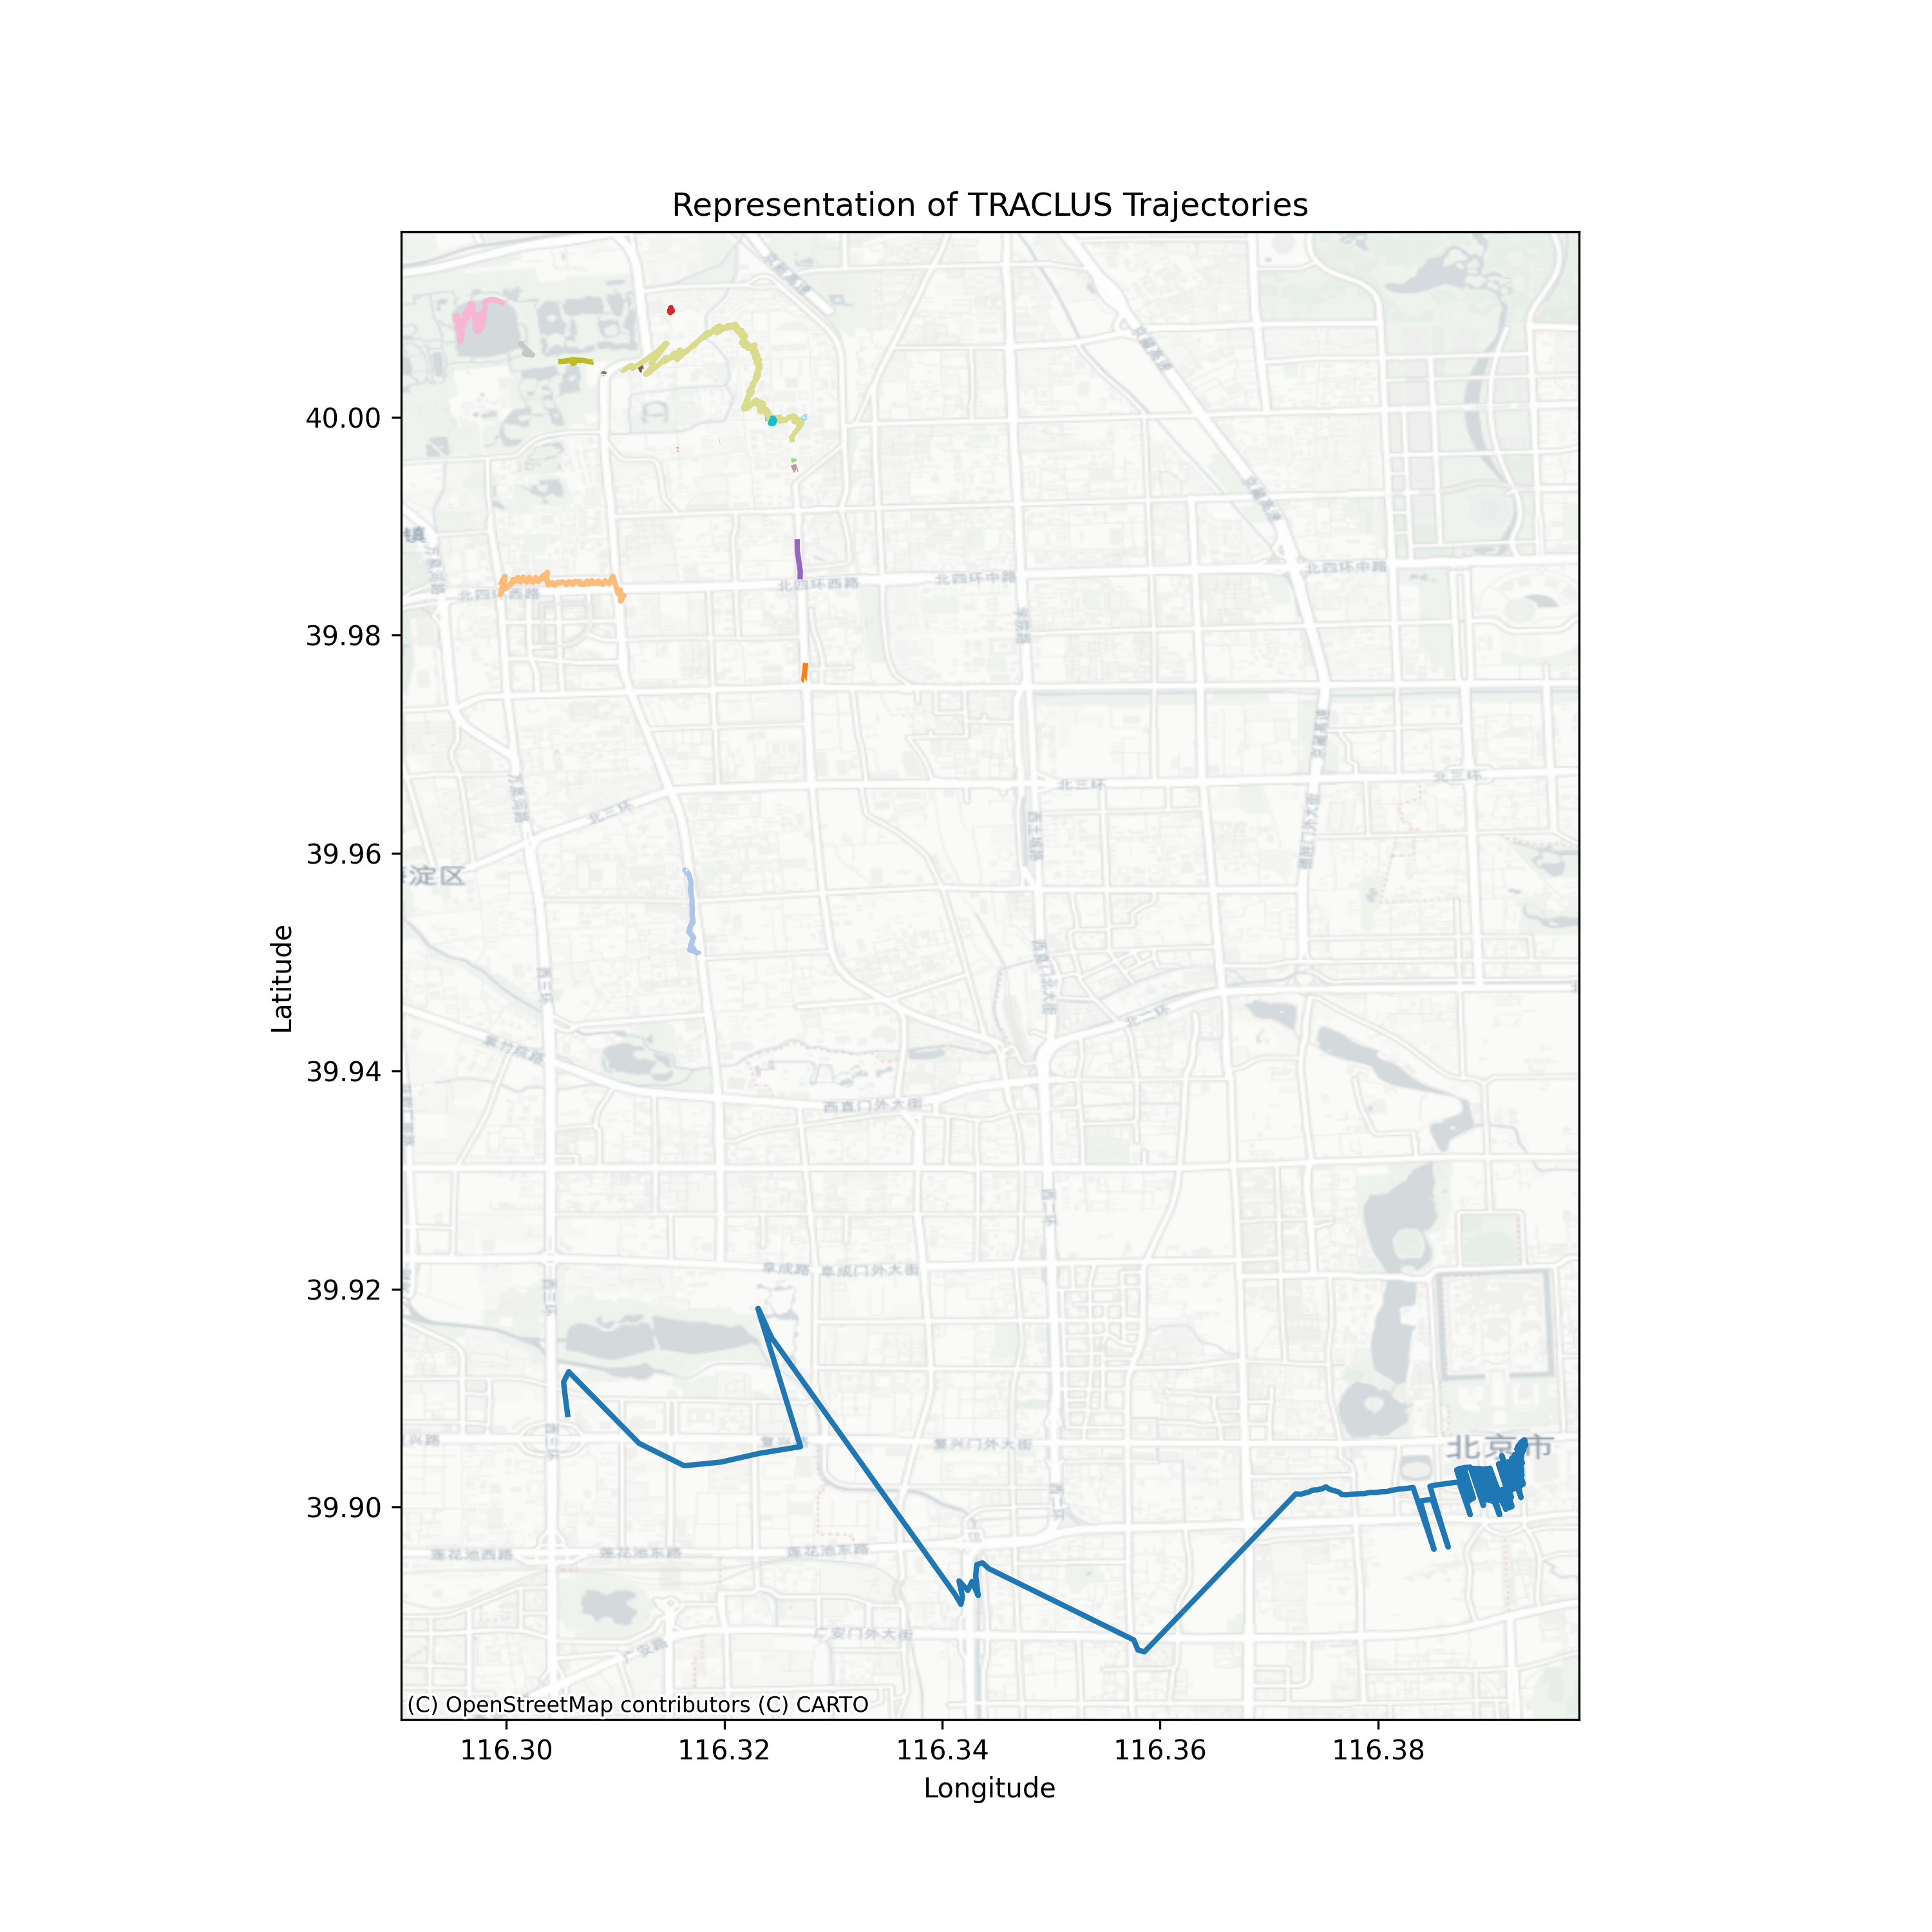
\includegraphics[width=0.5\textwidth]{img/Geolife/map_hdbscan_auto.png}
    \caption{Resultados con todos los algoritmos en HDBSCAN.}
    \label{fig:geolife_algorith_hdbscan}
\end{figure}

\FloatBarrier

La comparacion no es totalmente adecuada ya que aunque se haya usado el mismo numero de filas como el tiempo de ejecucion muestra la cantidad de datos no es la misma ya que cada cordenada cuanta para los calculos y los resultados.

Aun asi se puede ver como varían los resultados mucho mas depenciendo del algoritmo de clustering utilizado y que en concreto el parametro algotimn no tiene un impacto visible en el conjunto de datos analizado.


\paragraph{Max\_eps y eps}

Este parámetro determinó el rango máximo considerado para la agrupación en OPTICS y el rando determinado en DBSCAN. 

Por un lado DBSCAN produce cambios bastante significativos, el parametro eps debe estar entre 1 y 0, este es bastante común que falle, si se reduce mucho el numero es muy posible que no se encuentren datos que cumplan ese rango y por tanto no se pueda generar ningun resultado, por otro lado si se aumenta demasiado el numero se obtendrá el resultado contrario, todos los segmentos se agruparan en un solo cluster lo que hará los resultados inútiles.

\paragraph{Min\_sample}

Este parámetro controla el tamaño mínimo de los clústeres. En concreto se puede ver como las trayectorias resultantes se van separado unas de otras. Aumentar en gran medida este valor no parece conveniente ya que el centro del conjunto de datos aunque sea el mas poblado en cuanto a coordenadas termina desapareciendo acabando solo representados los bordes. Ademas si se aumenta en exceso se puede dar la condición de que solo uno de los clusters entre en las distancias o incluso ninguno y la operación falle.

En la siguiente imagen se puede vislumbrar como las coordenadas trayectoria resultantes se han ido disgragando en gran medida comparadas con las anterior representación de HDBSCAN en el conjunto de Movebank:

\begin{figure}[h!]
    \centering
    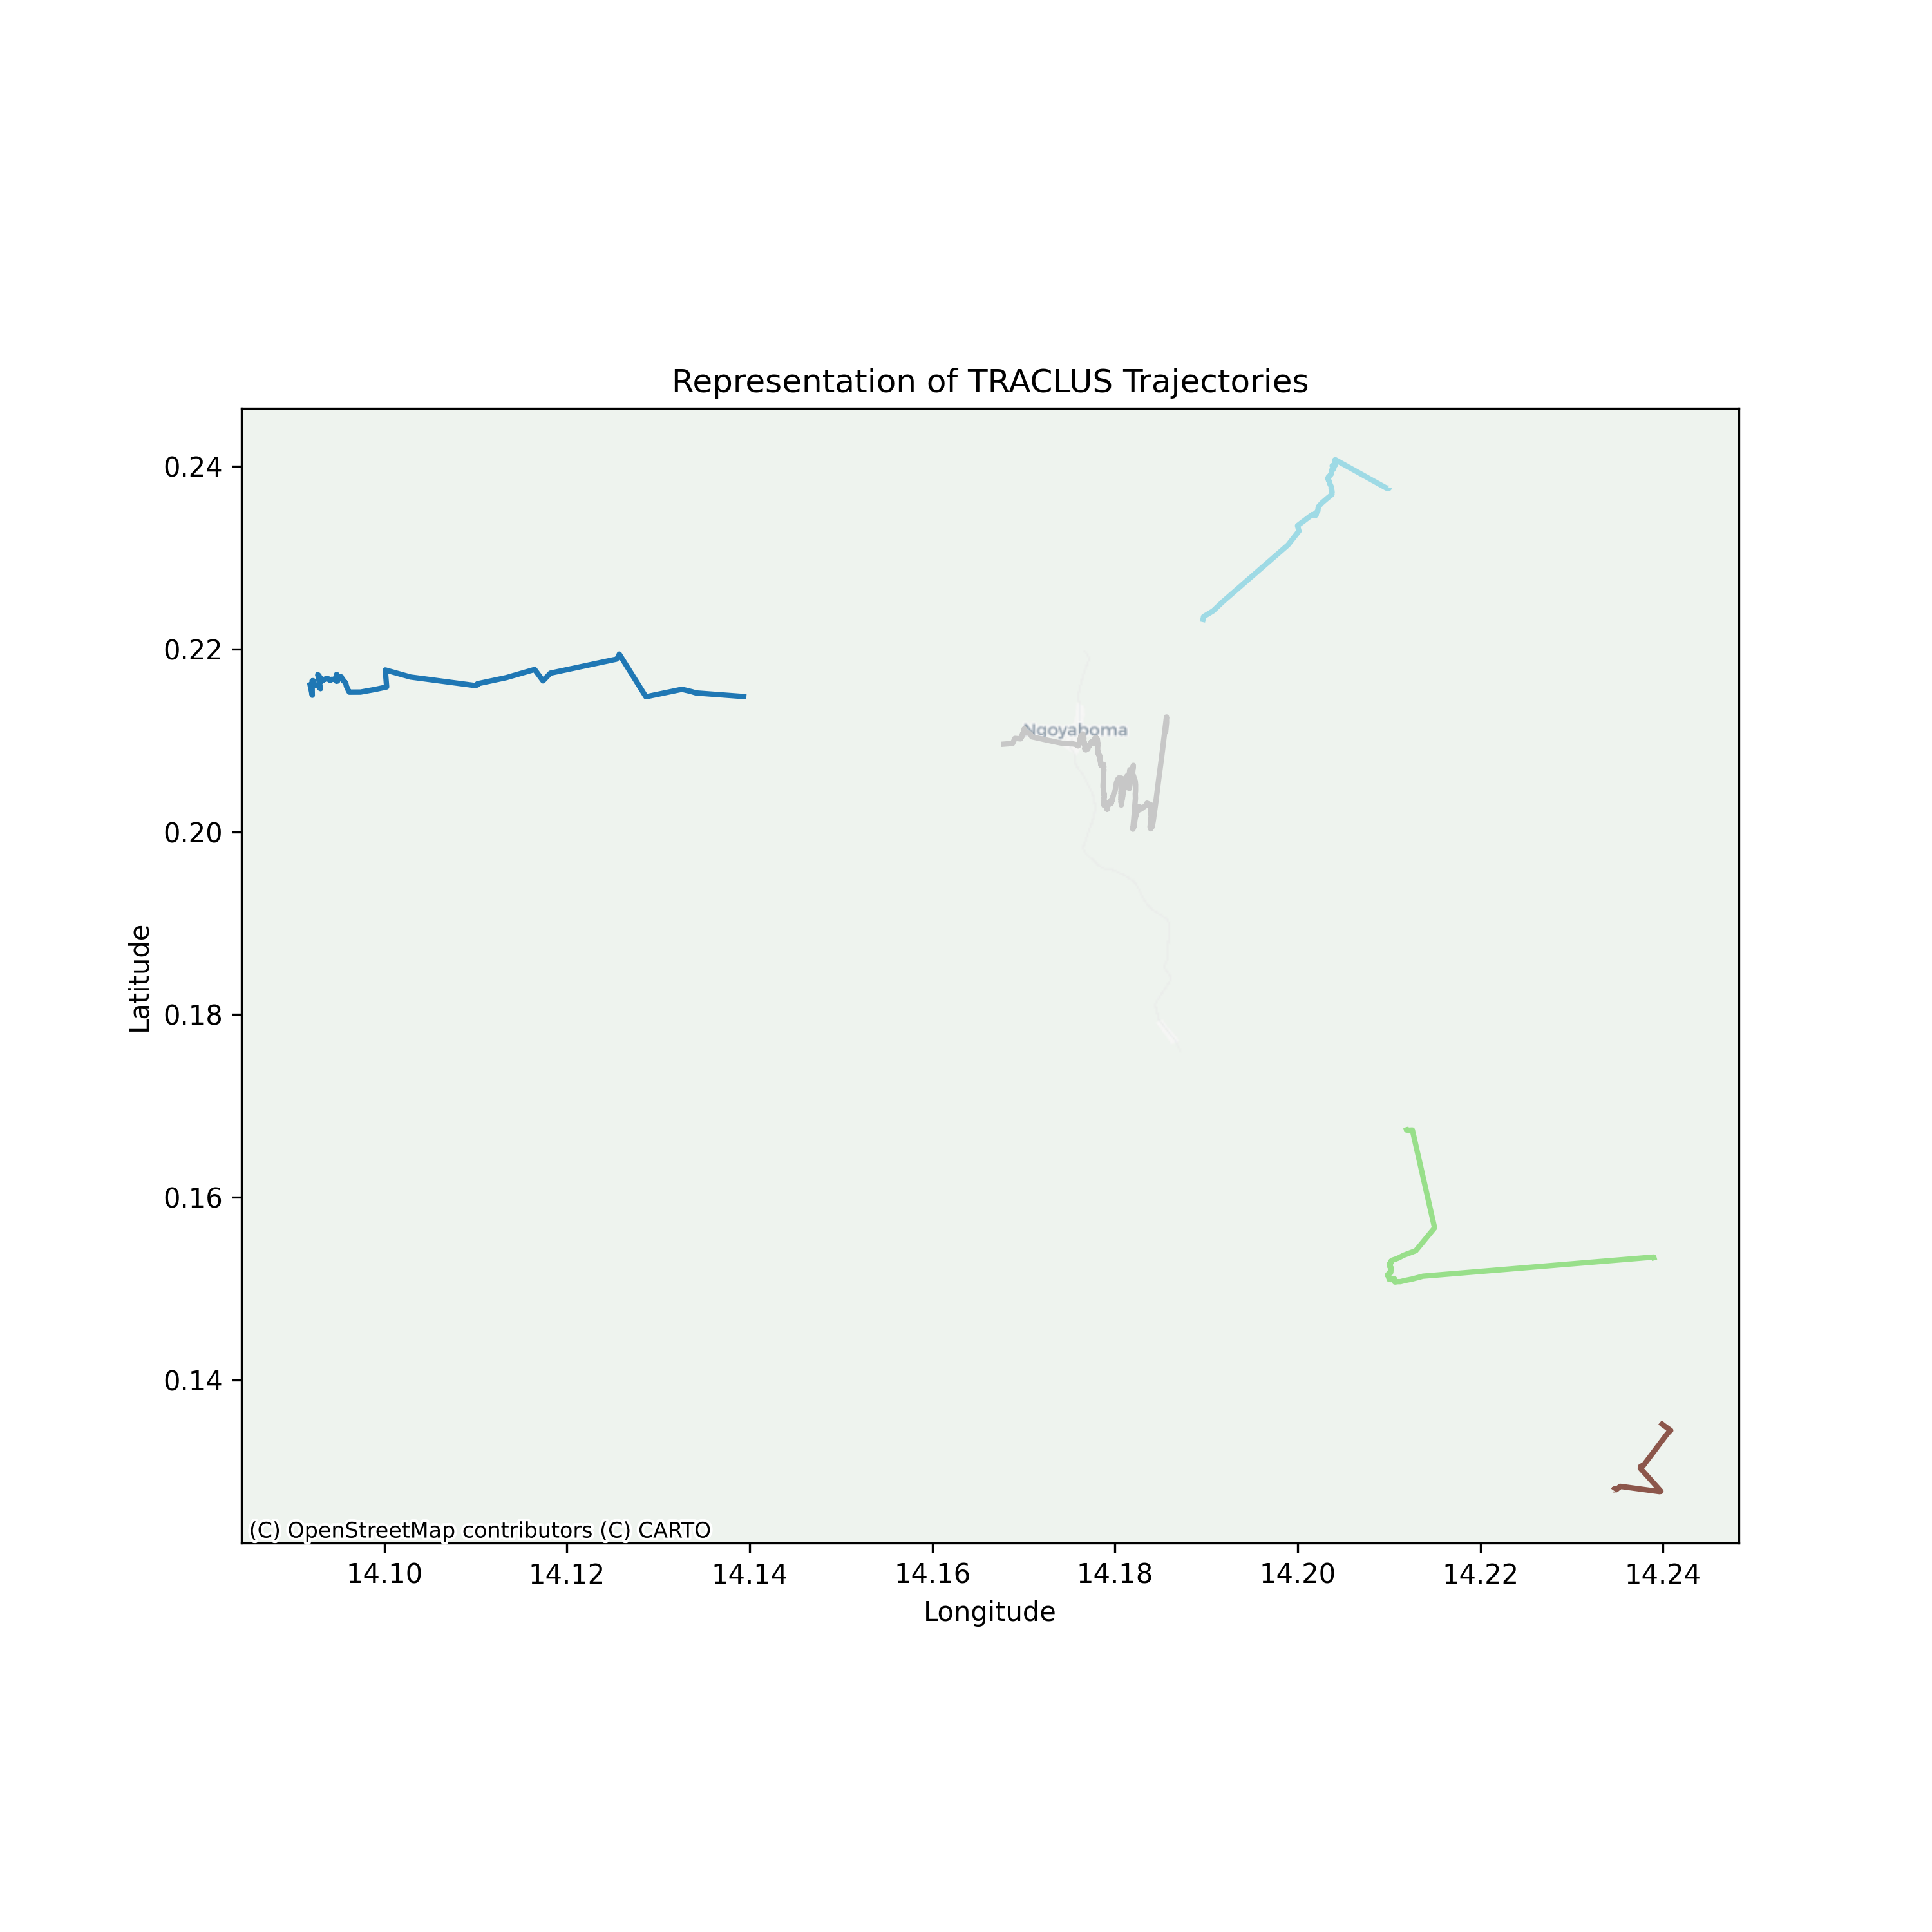
\includegraphics[width=0.5\textwidth]{img/Movebank/map_hdbscan_min.png}
    \caption{Resultados con aumento del $\min_{\text{sample}}$ en HDBSCAN.}
    \label{fig:min_sample}
\end{figure}

\subsubsection{Spectral y Agglomerative Clustering}

Aunque todos los parámetros pueden causar cambios en los resultados en Spectral y Agglomerative el numero de clusters seleccionado en el parámetro mas significativo. Esta cambia absolutamente el resultado y el tiempo de ejecución, cuando se le ponen cantidades bajas respecto a la cantidad de datos analizada los resultados bastante erráticos aunque si se pueden ver las zonas mas pobladas de coordenadas, ademas la transición de clusters a la representación de rutas no toma datos desechables por lo que si se van aumentano los clusters poco a poco el resultado comienza a se mas difícil de analizar, sin embargo llega a un punto en el que el programa comienza a catalogar clusters como desechables y los resutados pasan a ser mas acotados en ocasiones similares a los demas algoritmos o mucho mas pequeños.

\begin{figure}[h!]
    \centering
    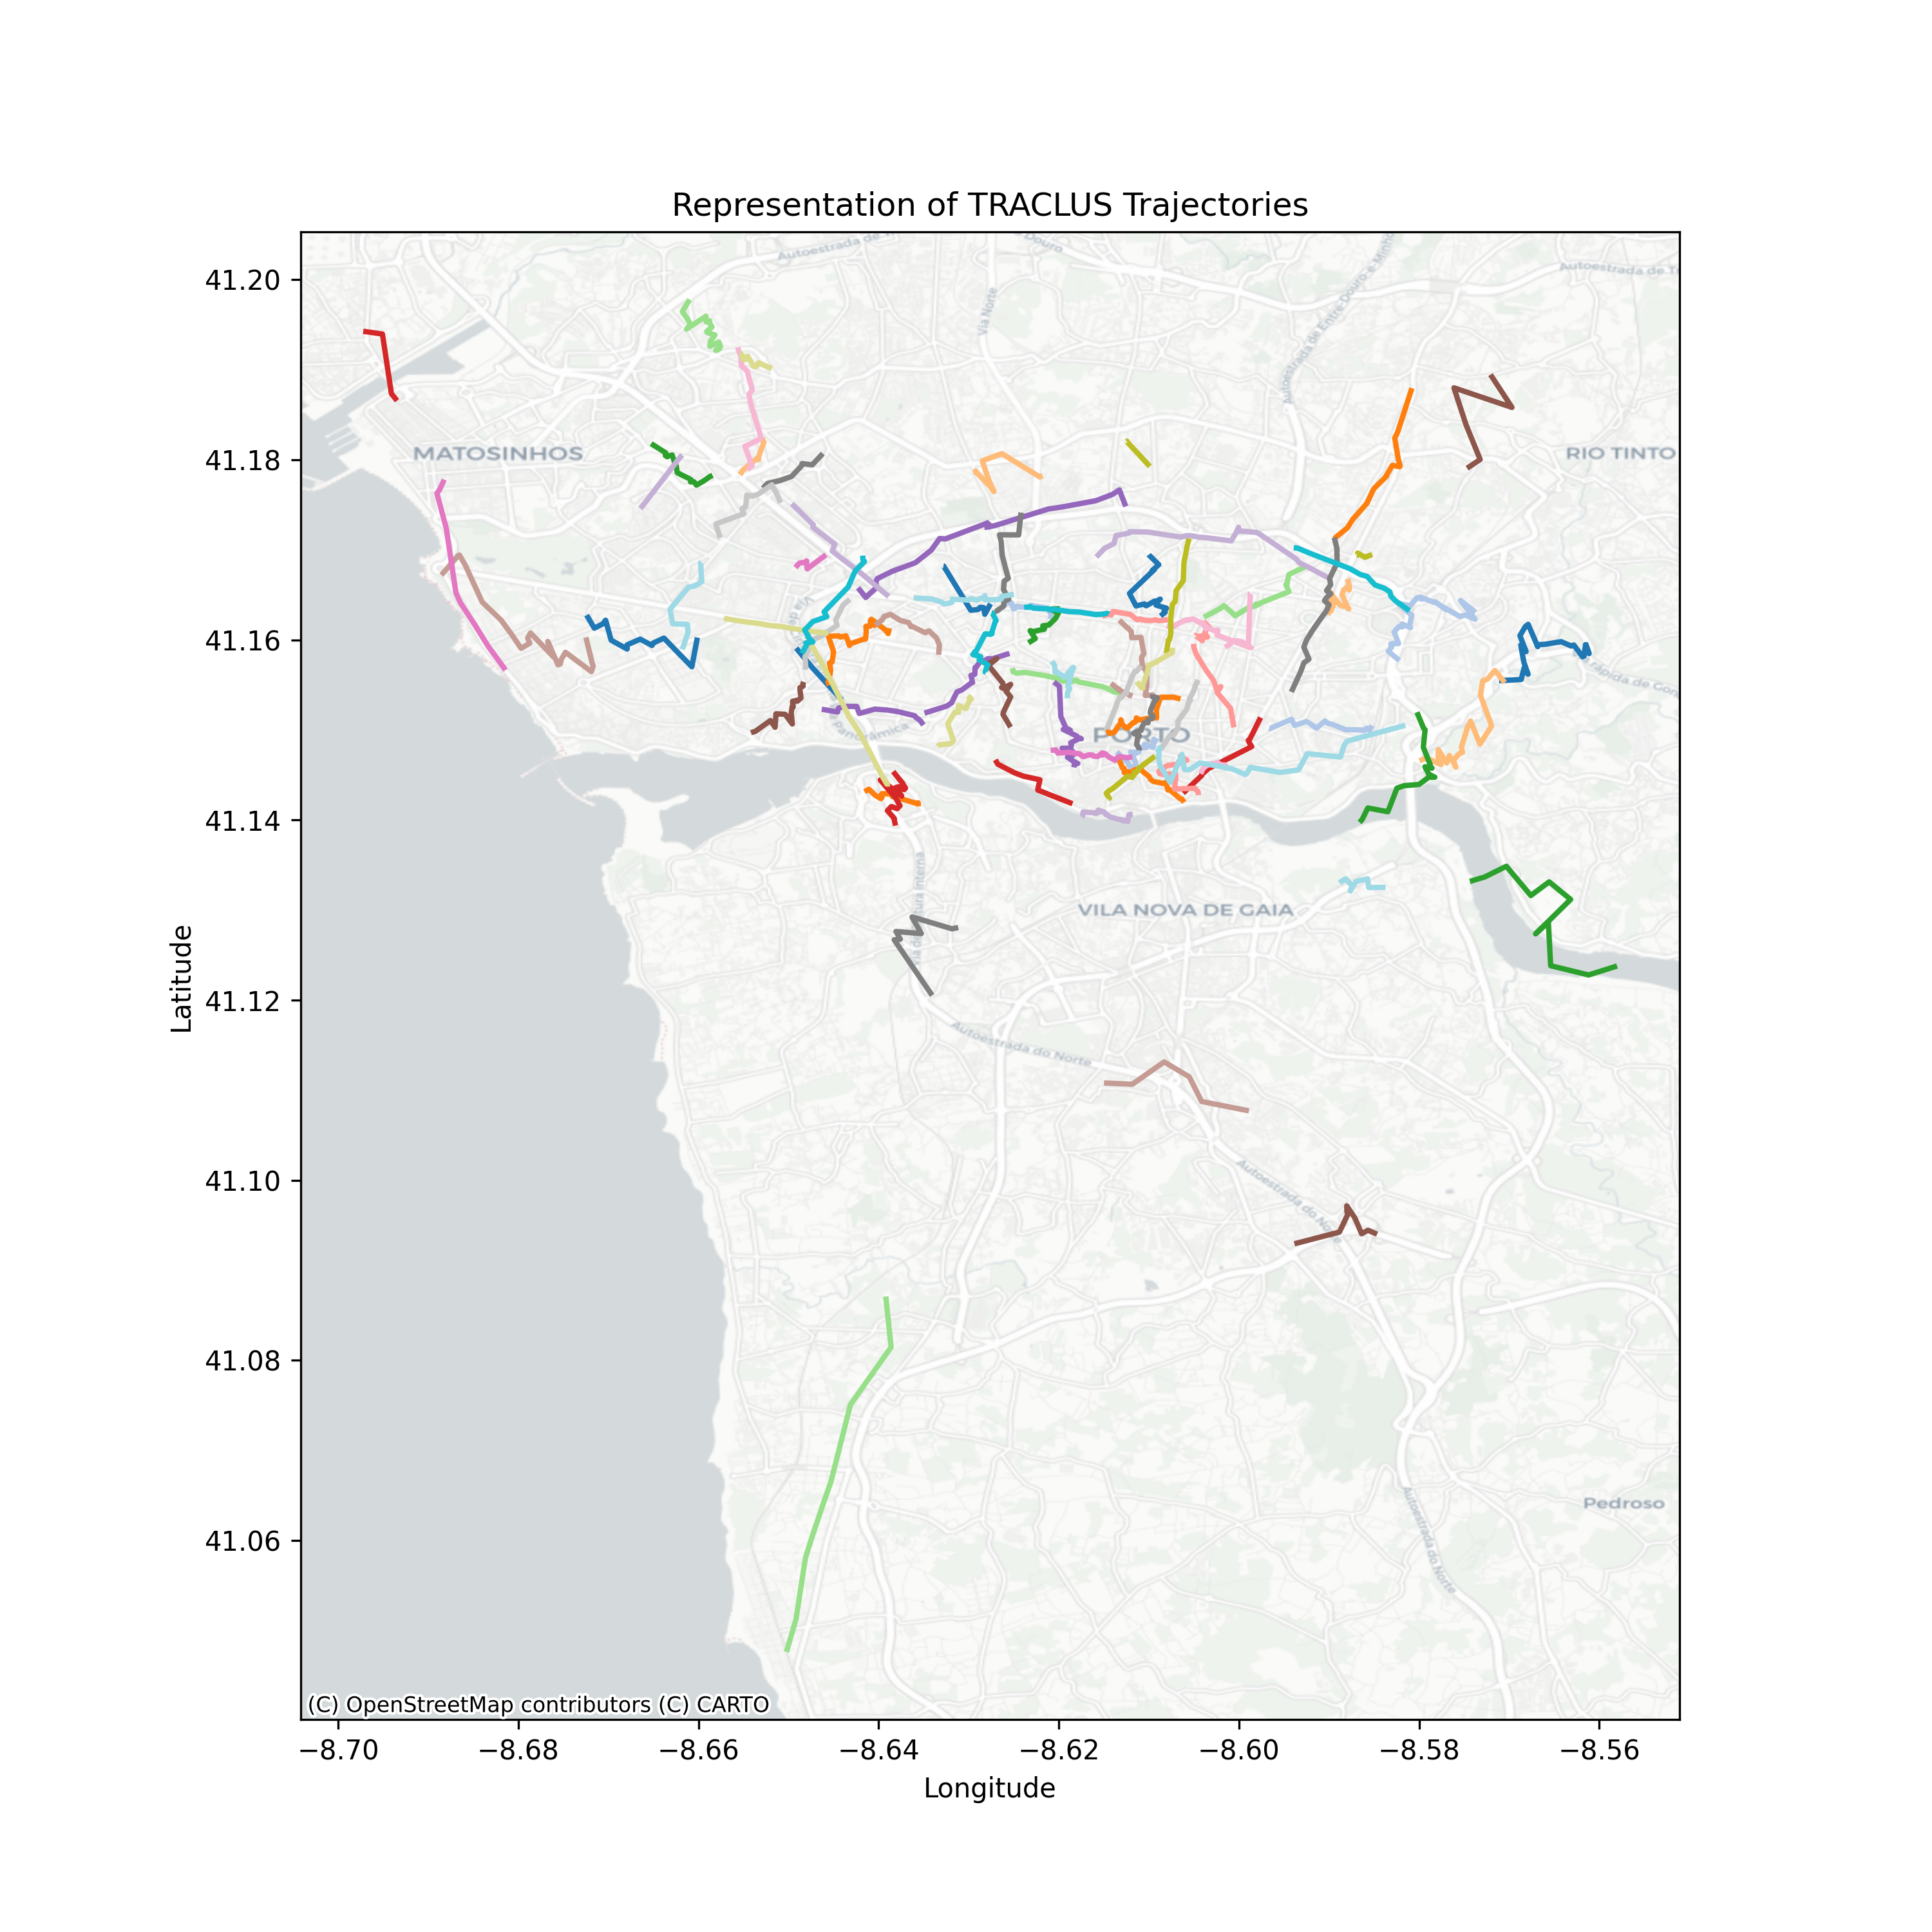
\includegraphics[width=0.5\textwidth]{img/Taxis/map_spect_90.png}
    \caption{Resultados con 90 clusters en Spectral.}
    \label{fig:spectral_90}
\end{figure}

\begin{figure}[h!]
    \centering
    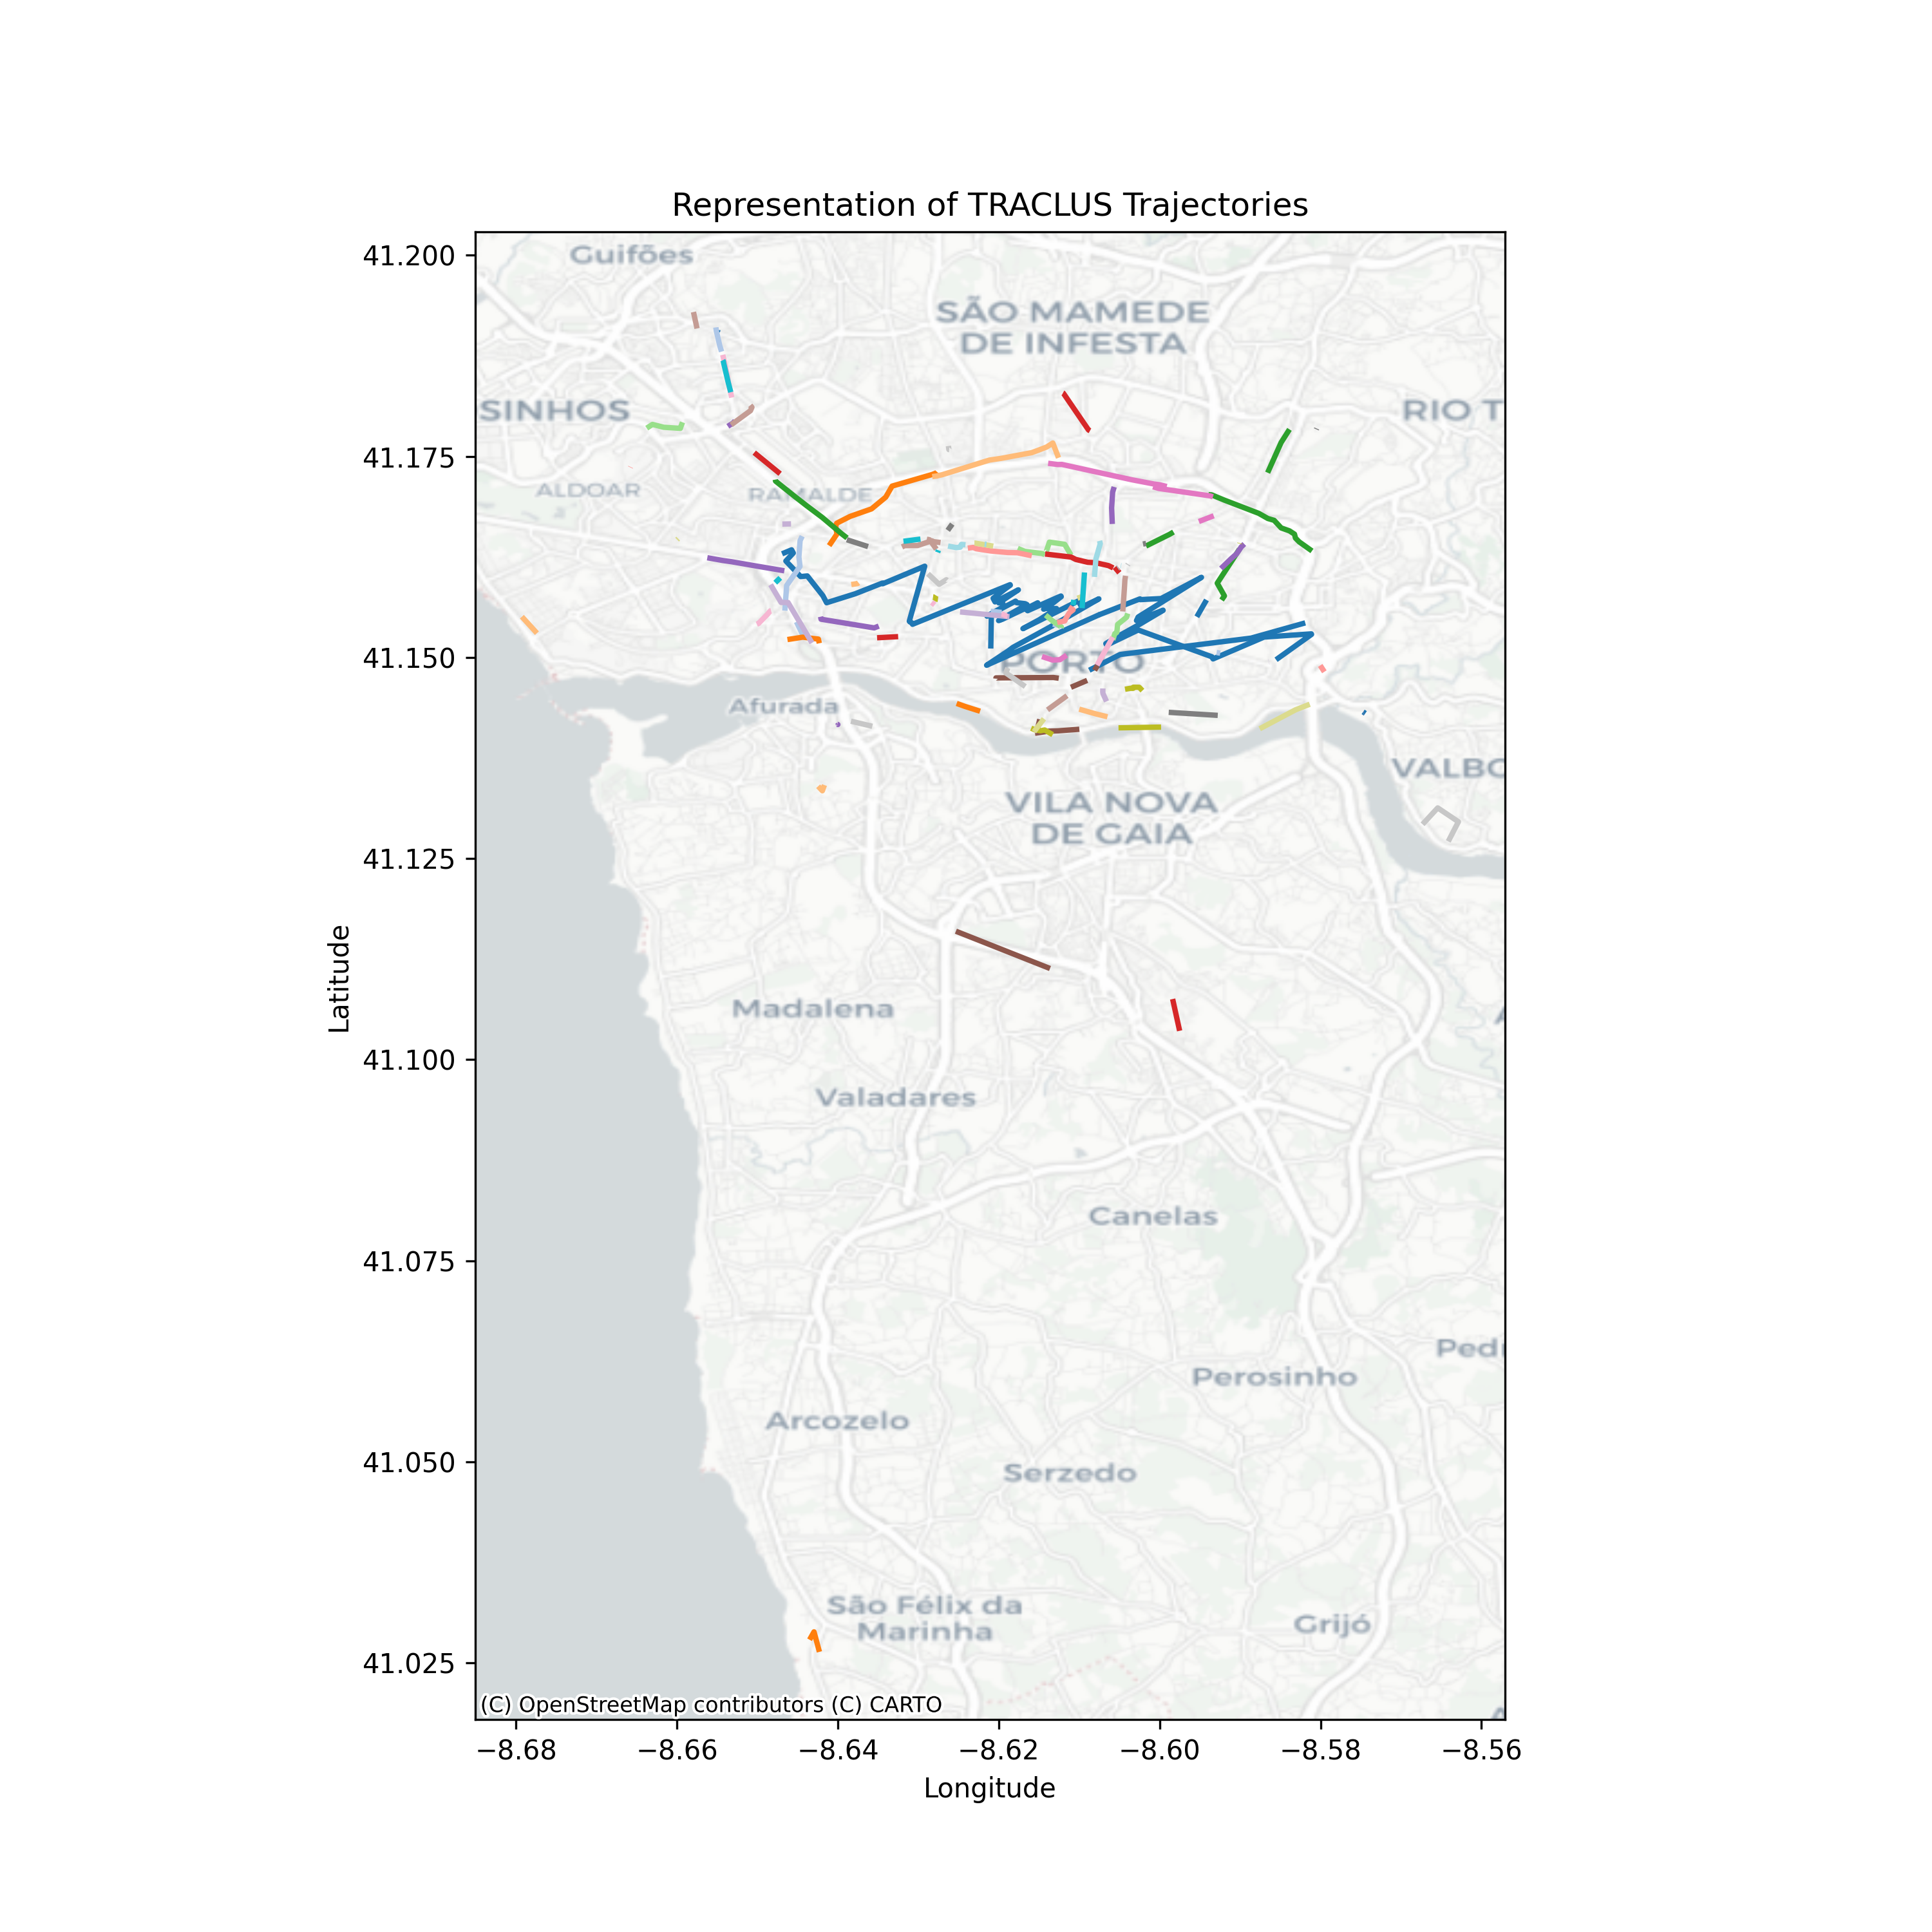
\includegraphics[width=0.5\textwidth]{img/Taxis/map_spect_500.png}
    \caption{Resultados con 500 clustes en Spectral.}
    \label{fig:spetral_500}
\end{figure}

\begin{figure}[h!]
    \centering
    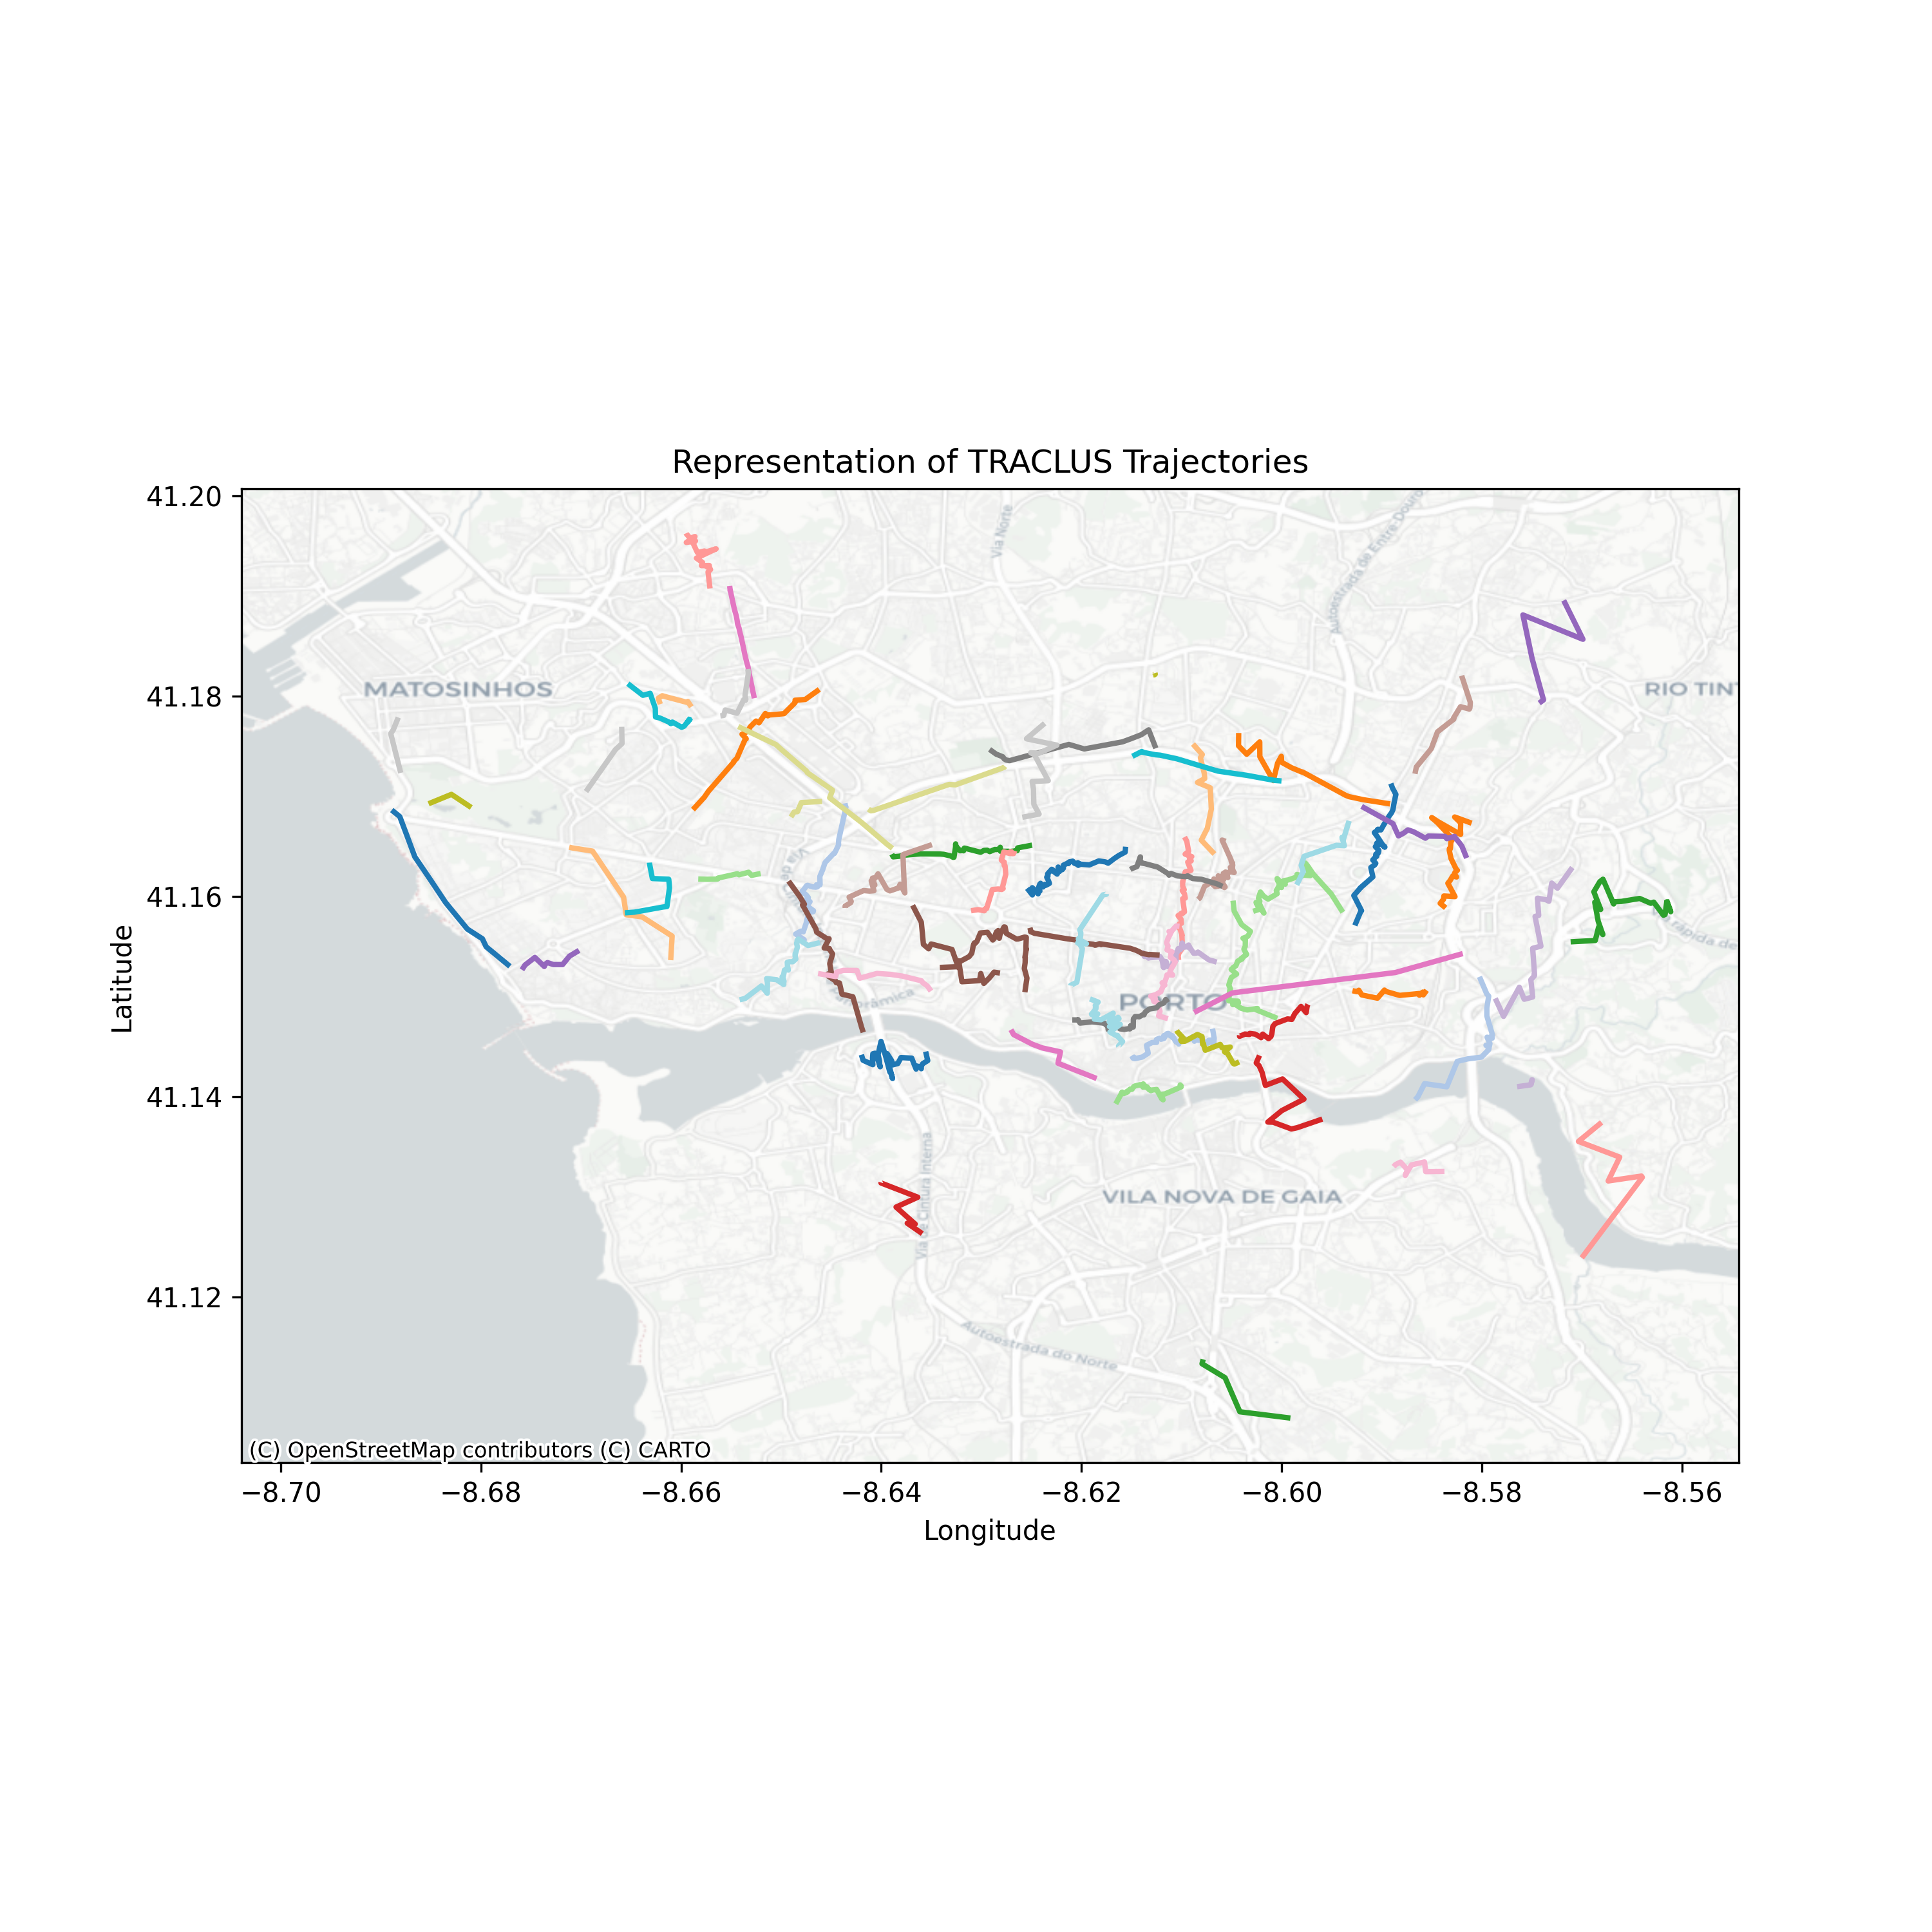
\includegraphics[width=0.5\textwidth]{img/Taxis/map_agglo_90.png}
    \caption{Resultados con 90 clusters en Agglomerative.}
    \label{fig:agglo_90}
\end{figure}

\begin{figure}[h!]
    \centering
    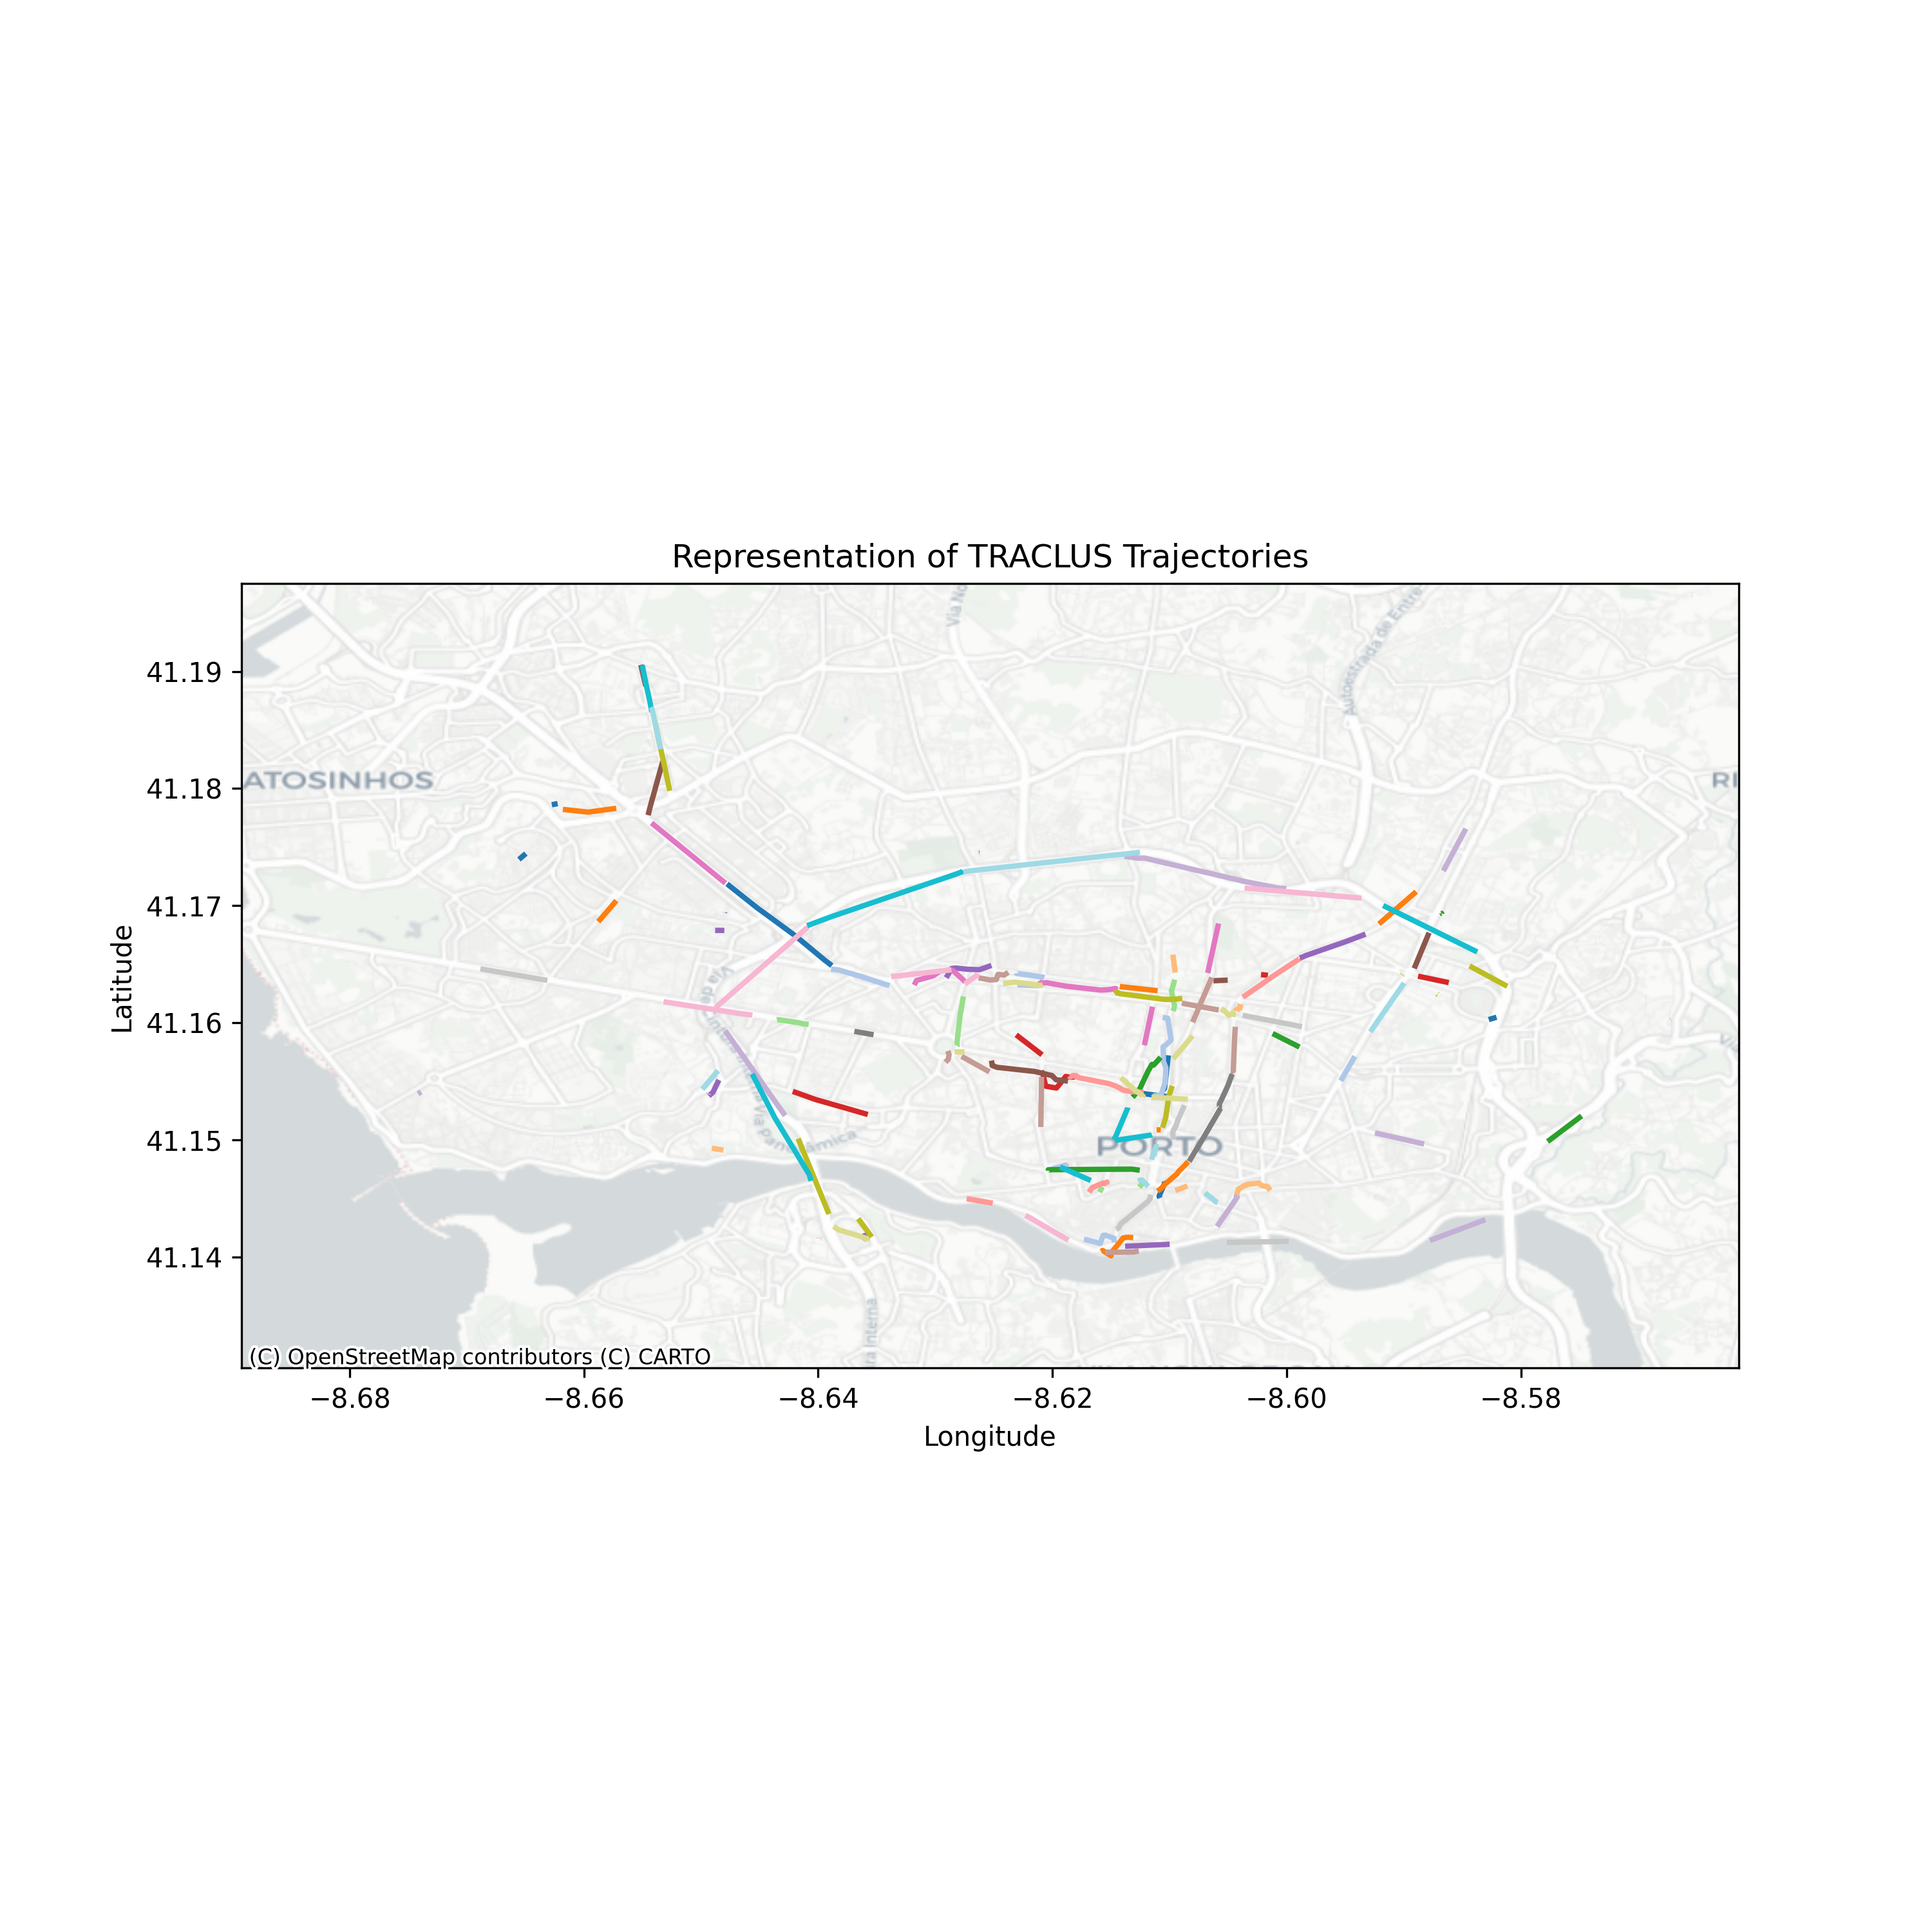
\includegraphics[width=0.5\textwidth]{img/Taxis/map_agglo_500.png}
    \caption{Resultados con 500 clustes en Agglomerative.}
    \label{fig:agglo_500}
\end{figure}

Los otros parametros no se quedan tan atras en modificacion de los resultados. En ambios la agrupecion de los clusters se ve con multiples variaciones llegango ha hacer resultados vastante erraticos.

\begin{figure}[h!]
    \centering
    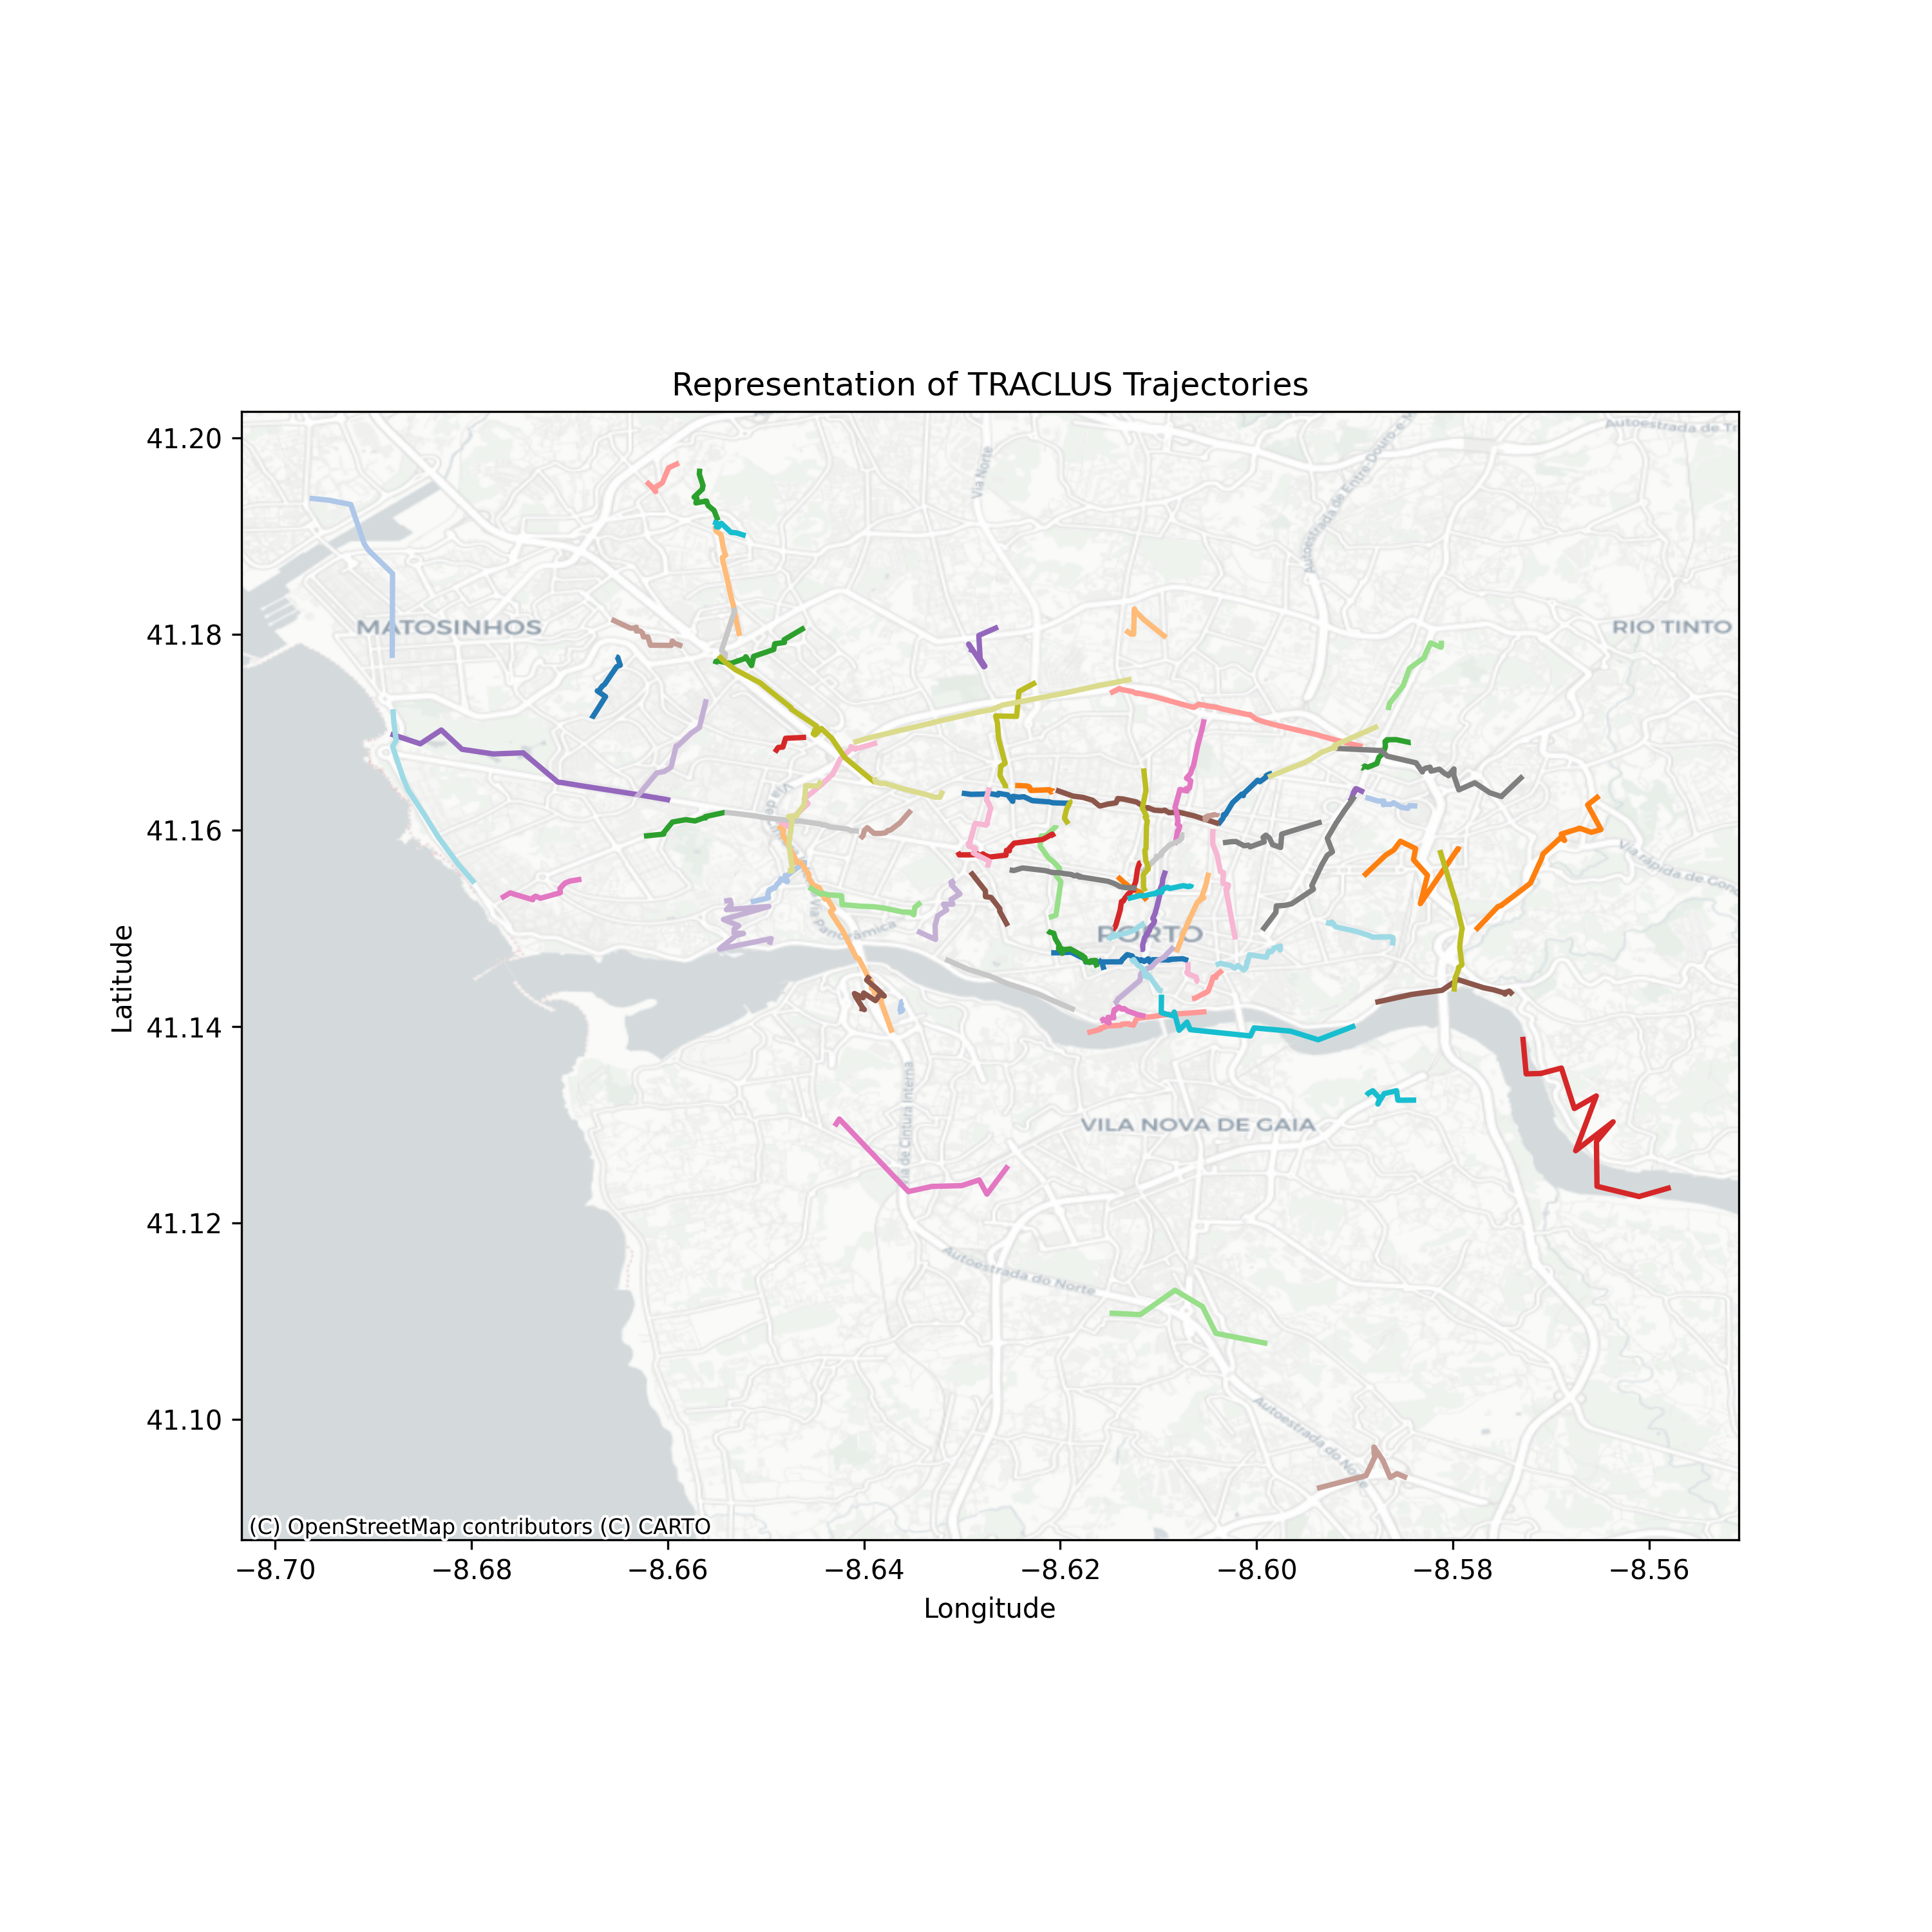
\includegraphics[width=0.5\textwidth]{img/Taxis/map_spect_par.png}
    \caption{Resultados con 90 clusters, $\text{precomputed}_{\text{nearest\_neighbors}}$ y discretize en Spectral.}
    \label{fig:spectal_par}
\end{figure}

\begin{figure}[h!]
    \centering
    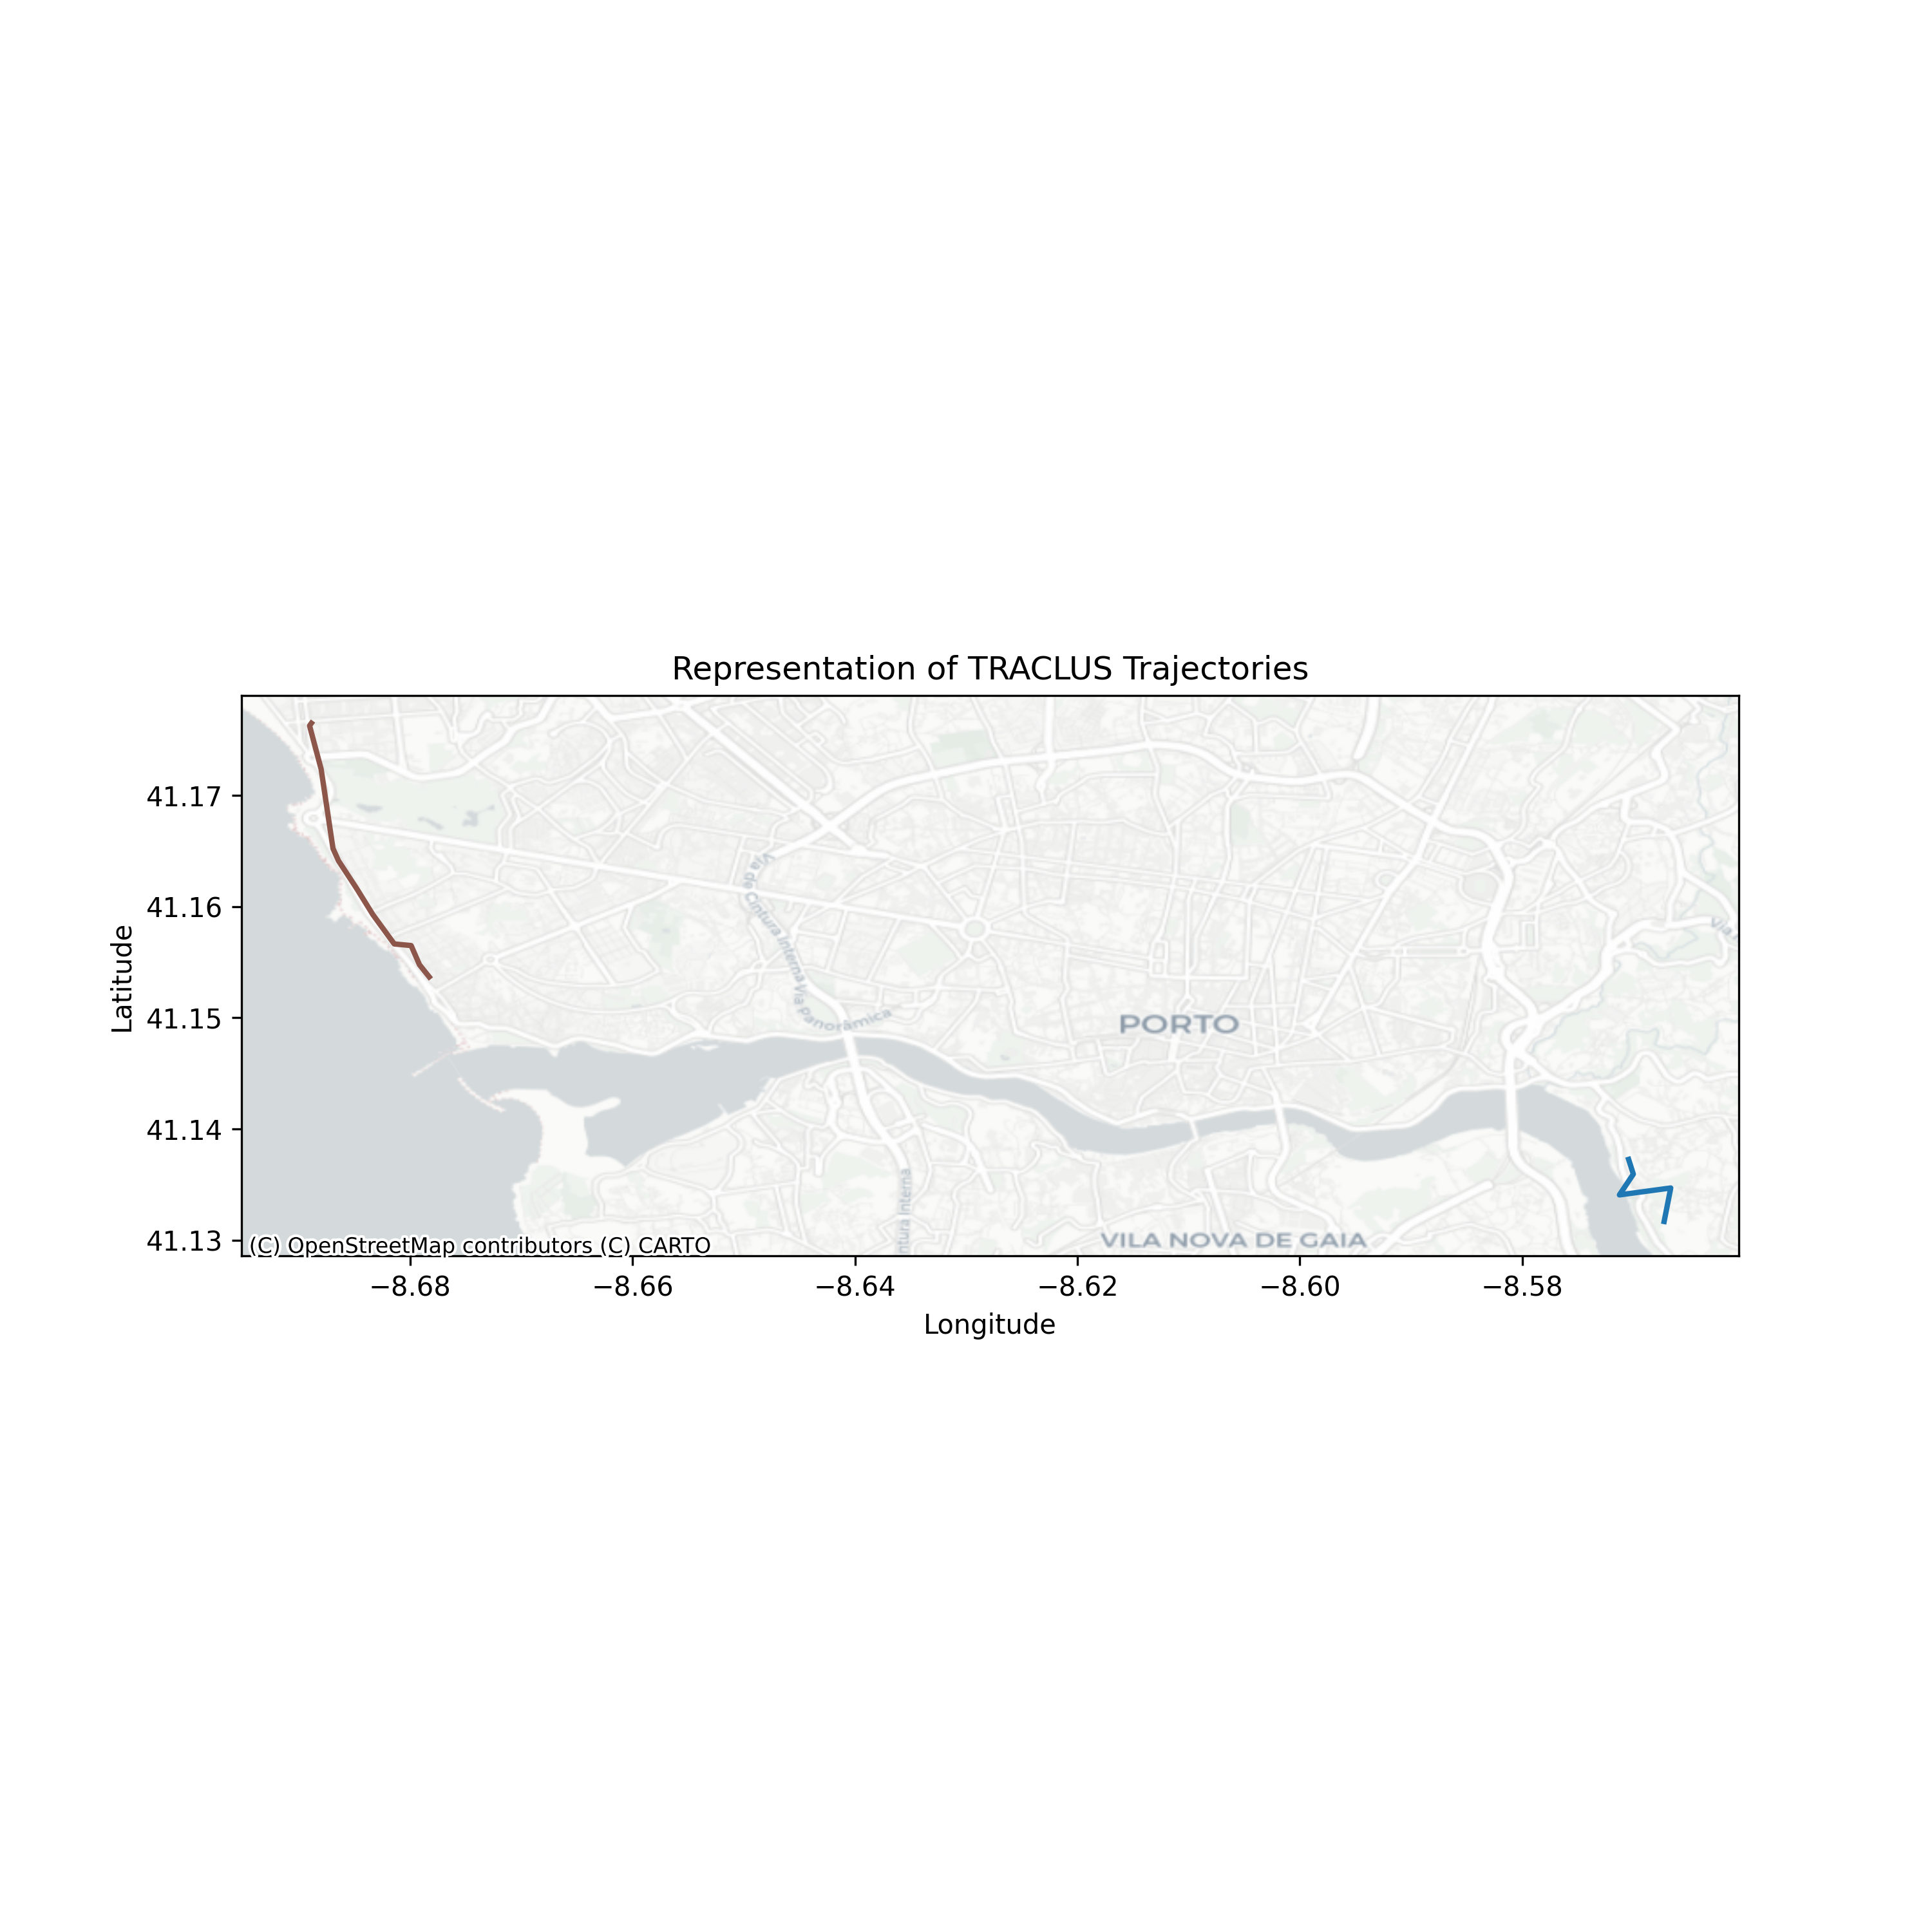
\includegraphics[width=0.5\textwidth]{img/Taxis/map_agglo_par.png}
    \caption{Resultados con 90 clustes y single en Agglomerative.}
    \label{fig:agglo_par}
\end{figure}

\subsection{Conclusión}

Aunque todos los algoritmos analizados muestran cierta utilidad, y aunque se podrían realizar pruebas más exhaustivas y variadas, es posible extraer algunas conclusiones preliminares.

\begin{table}[ht]
\centering
\begin{tabular}{|l|c|c|c|}
\hline
\textbf{Algoritmos} & \textbf{Trayectorias Taxis (seg)} & \textbf{MoveBank (seg)} & \textbf{Geolife (seg)}  \\
\hline
OPTICS & 344 & 766 & 3871 \\
DBSCAN & 327 & 767 & 4048 \\
HDBSCAN & 478 & 865 & 4947 \\
Spectral Clustering & 469 & 928 & 4758 \\
Agglomerative Clustering & 465 & 917 & 4757 \\
\hline
\end{tabular}
\caption{Tiempos de ejecución de los algoritmos en segundos}
\label{tabla:comparacion_algoritmos}
\end{table}

Para aplicaciones en tiempo real o con grandes volúmenes de datos, los algoritmos Spectral y Agglomerative no son recomendables, ya que su tiempo de ejecución aumenta considerablemente. Para obtener resultados más claros, estos métodos requieren un número elevado de clústeres, lo que incrementa aún más el tiempo de procesamiento.

Además, la necesidad de ajustar los parámetros según el tamaño y las características de cada conjunto de datos es otro desafío. En este contexto, HDBSCAN destaca por su versatilidad, dado que determina automáticamente tanto el número como el tamaño de los clústeres. Sin embargo, esta flexibilidad tiene un costo: los resultados fueron en ocasiones poco interpretables, y el tiempo de ejecución superó al de OPTICS y DBSCAN.

Por otro lado, OPTICS demostró ser consistente y eficiente en todos los escenarios evaluados, lo que respalda su elección como algoritmo preferido en las pruebas iniciales.

Finalmente, DBSCAN tiende a crear un número reducido de clústeres, concentrándose principalmente en las regiones de mayor densidad y rechazando segmentos menos poblados. Esta característica, compartida en cierta medida con los algoritmos Spectral y Agglomerative, se manifiesta de manera opuesta: mientras DBSCAN agrupa solo las áreas más densas, Spectral y Agglomerative distribuyen clústeres de manera amplia, pero con una representatividad reducida a medida que aumenta su número.












\apendice{Anexo de sostenibilización curricular}

\section{Introducción}
Este proyecto se alinea con varios Objetivos de Desarrollo Sostenible (ODS)~\cite{ODS} definidos por Naciones Unidas en 2015. Dichos objetivos buscan erradicar la pobreza, proteger el planeta y asegurar la prosperidad para todos como parte de una agenda global con metas a alcanzar en 2030. A continuación, se detalla cómo este proyecto contribuye a algunos de los ODS seleccionados.

\section{Objetivo número 4: Educación de calidad}
El desarrollo de esta aplicación web fomenta el aprendizaje y la accesibilidad de información técnica para el análisis de datos geográficos y temporales. Esto permite a estudiantes, investigadores y profesionales acceder a herramientas que antes podrían haber requerido conocimientos avanzados o recursos costosos. La democratización del acceso a estas herramientas fomenta una educación más inclusiva y accesible.

\subsection{Impacto en la práctica}
\begin{itemize}
    \item Formación técnica: Proporciona una plataforma para que los usuarios desarrollen habilidades prácticas en análisis de datos y visualización geoespacial.
    \item Inclusión educativa: Facilita el acceso a tecnologías avanzadas para comunidades con recursos limitados, ampliando las oportunidades de aprendizaje.
    \item Colaboración interdisciplinaria: Promueve el uso de tecnologías en áreas como la educación, la geografía y la sostenibilidad, fomentando proyectos colaborativos entre disciplinas.
\end{itemize}

\section{Objetivo número 9: Industria, innovación e infraestructura}
La creación de una aplicación optimizada para el análisis geoespacial y la gestión de datos temporales refuerza la importancia de la innovación en la digitalización de procesos tradicionales. Este proyecto promueve una infraestructura tecnológica accesible y eficiente, que puede ser replicada y adaptada para diversos contextos.

\subsection{Impacto en la práctica}
\begin{itemize}
    \item Promoción de herramientas sostenibles: La aplicación está diseñada para ser reutilizable y adaptable a distintos escenarios, minimizando la necesidad de crear nuevas herramientas desde cero.
    \item Innovación tecnológica: Utiliza técnicas avanzadas en visualización y análisis de datos para resolver problemas prácticos en diversas áreas de investigación.
    \item Eficiencia en la gestión de recursos: Al centralizar y procesar datos complejos en una sola plataforma, se reduce el tiempo y los recursos necesarios para realizar análisis.
\end{itemize}

\section{Objetivo número 13: Acción por el clima}
Aunque no de manera directa, este proyecto contribuye a la acción por el clima al facilitar la comprensión y el análisis de datos geoespaciales que pueden ser utilizados para estudios relacionados con el medio ambiente. Por ejemplo, permite analizar patrones de movilidad, cambios en el uso del suelo o distribución de eventos climáticos extremos, proporcionando información valiosa para la toma de decisiones sostenibles.

\subsection{Impacto en la práctica}
\begin{itemize}
    \item Análisis ambiental: Permite a los usuarios identificar patrones y tendencias en datos geográficos que pueden relacionarse con el cambio climático.
    \item Sensibilización: Al integrar datos geoespaciales con visualizaciones claras, ayuda a comunicar la urgencia de acciones relacionadas con el medio ambiente.
    \item Reducción de recursos: La herramienta digitaliza procesos que antes requerían análisis manuales o múltiples plataformas, disminuyendo el consumo de recursos materiales y energía.
\end{itemize}

\section{Conclusión}
Este proyecto no solo cumple con su propósito de ofrecer una herramienta eficiente para el análisis y visualización de datos geográficos, sino que también contribuye al avance de varios Objetivos de Desarrollo Sostenible. Al fomentar la educación inclusiva, la innovación tecnológica y la acción climática, este trabajo demuestra cómo pequeñas iniciativas pueden tener un impacto significativo en el logro de metas globales.





\bibliographystyle{plain}
\bibliography{bibliografiaAnexos}

\end{document}
